\documentclass{beamer}
\usepackage[utf8]{inputenc}
\usepackage{tabularx}
\usepackage{mathrsfs}
\usepackage{pgf}


\usepackage{amsmath}
\usepackage{amsmath,times} %% times package needed only to load TNR text font
\usepackage{array}
\usepackage{pifont}% http://ctan.org/pkg/pifont
\newcommand{\cmark}{\ding{51}}%
\newcommand{\xmark}{\ding{55}}%
% \usepackage{enumitem}
\usepackage[ruled]{algorithm2e}
\usepackage{underoverlap}
% \usepackage{algorithm}
\usepackage{algpseudocode}
\usepackage{tabularx}
\usepackage{mathrsfs}
\usepackage{pgf}
\usepackage{amsmath}
\usepackage{array}
\usepackage{tabularx}
\usepackage[nointegrals]{wasysym}
\usepackage{xcolor,colortbl}

\usepackage{multirow}
\usepackage{adjustbox}
\usepackage{booktabs}
\usepackage{subfig}

\usepackage{pifont}% http://ctan.org/pkg/pifont
\usepackage{tikz}
\usetikzlibrary{calc, chains, decorations.pathmorphing}
\usetikzlibrary{shapes.geometric}
\usetikzlibrary{arrows,shapes,positioning}
\usetikzlibrary{shapes.symbols}
\usetikzlibrary{calc,decorations.markings}
\usetikzlibrary{decorations.text}
\usetikzlibrary{patterns}
\usetikzlibrary{fit}
\usetikzlibrary{arrows.meta}
\usetikzlibrary{plotmarks}
\usepackage{color, soul}

\definecolor{top-darkblue}{RGB}{62,78,99} 
\definecolor{foot-darkblue}{RGB}{77,82,151} 
\definecolor{foot-blue}{RGB}{171,200,230} 
\definecolor{title-blue}{RGB}{0,76,153}

\definecolor{block-red}{rgb}{1.1, 0.41, 0.38}
\definecolor{propa-grey}{rgb}{0.82, 0.84, 0.86}
\definecolor{true-green}{RGB}{182,191,0}%{rgb}{0, 0.8, 0.2}
\definecolor{purple}{rgb}{0.74, 0.2, 0.64}
\definecolor{cons-red}{rgb}{0.5, 0.11, 0.11}

\definecolor{UPMCEngagementBlueA} {RGB}{140,184,198}
\definecolor{UPMCEngagementBlueB} {RGB}{92,127,146}

\definecolor{UPMCCorporateGreen} {RGB}{182,191,0}
\definecolor{UPMCExcellenceOrangeA} {RGB}{224,82,6}
\definecolor{UPMCExcellenceOrangeB} {RGB}{225,160,47}

\mode<presentation> {
  \usetheme[not@ku={UPMC}, wide, TPomitframeno, FTalign=left,%
  greyfoot, fnolabel=, basecolour=UPMCEngagementBlueB,%
  sidebar=0pt]{Frederiksberg}
  \setbeamercolor{block title example}{bg=UPMCCorporateGreen}
  \setbeamercolor{block title alerted}{bg=UPMCExcellenceOrangeA}
  \setbeamercolor{alerted text}{fg=UPMCExcellenceOrangeA}
  \setbeamertemplate{headline}{}
  \setbeamertemplate{footline}[page number]{}
  \setbeamercovered{transparent}
  \beamertemplatenavigationsymbolsempty
}

\definecolor{red}{rgb}{0.7, 0.11, 0.11}
\definecolor{green}{rgb}{0, 0.8, 0.2}

\tikzstyle{point}=[circle,draw,thick,fill=black,scale=0.2]
\tikzstyle{point+}=[circle,draw=red,thick,fill=red,scale=0.3]
\tikzstyle{class2}=[ellipse, draw, minimum width=2cm, minimum height=1cm]
\tikzstyle{class1}=[ellipse, draw, minimum width=1cm, minimum height=1cm]

\tikzstyle{decision}=[circle,draw,thick,fill=UPMCEngagementBlueA]
\tikzstyle{decision-graph}=[text width={width("$\neg x_3@3$")},circle,
align=center,draw,thick,fill=yellow]
\tikzstyle{propa-graph}=[text width={width("$\neg x_3@3$")},circle,draw,thick,
align=center,fill=propa-grey]
\tikzstyle{conflict}=[<->,>=latex,rounded corners=5pt,thick,draw=blue, line width=1mm]
\tikzstyle{uip}=[draw=true-green,ultra thick]
\tikzstyle{cut}=[-,>=stealth,rounded corners=5pt,thick,draw=blue, line width=0.4mm]
\tikzstyle{link}=[->,>=latex,rounded corners=5pt,thick]
\tikzstyle{unsat}=[draw,thick,fill=red]
\tikzstyle{sat}=[draw,thick,fill=green]
\tikzstyle{propa}=[draw,thick,fill=propa-grey]
\tikzstyle{backtrack}=[->,>=latex,dashed,rounded corners=20pt,thick,draw=blue, line width=0.5mm]

\setbeamertemplate{footline}[frame number]{}

% Definition of variable
\def\SAT{\textcolor{green}{\texttt{SAT}}}
\def\UNSAT{\textcolor{red}{\texttt{UNSAT}}}

\def\true{\textcolor{green}{\texttt{true}}}
\def\false{\textcolor{red}{\texttt{false}}}

\def\ok{\textcolor{green}{\cmark}}
\def\ko{\textcolor{red}{\xmark}}




\begin{document}

\author{Hakan \textsc{METIN}}


\begin{frame}
\frametitle{Exploitation of dynamic symmetries for solving SAT problems}
%\frametitle{Exploitation des symétries dynamiques pour la résolution des problèmes SAT}
\framesubtitle{Doctorat de Sorbonne Université}

   Hakan \textsc{Metin} \hfill {\scriptsize  Le, 18 décembre 2019}\\
  \vfill
  %\begin{center}

	\scriptsize
    \begin{tabular}{ll}
 	    \textbf{Rapporteurs:} & \\
    	\textsc{Pascal \textsc{Fontaine}}  & Professeur, Université de Liège\\
    	\vspace{1em}%
    	\textsc{Laure Petrucci}  & Professeur, Université Paris 13\\

 	    \textbf{Examinateurs:} & \\
   		\textsc{Bart Bogaerts} & Assistant Professor, Vrije Universiteit Brussel\\
    	\textsc{Jean-Michel	Couvreur}  & Professeur, Université d'Orléans\\
    	\vspace{1em}%
    	\textsc{Emmanuelle Encrenaz}  & Maître de conférences, Sorbonne Université\\




 	    \textbf{Directeurs:} & \\
    	\textsc{Souheib Baarir}  & Maître de conférences, Université Paris Nanterre\\
    	\textsc{Fabrice Kordon}  & Professeur, Sorbonne Université\\
    \end{tabular}\\
 % \end{center}

  \vskip 3ex
  \begin{columns}[t]
    \begin{column}[T]{\textwidth}
      
\includegraphics[height=1.2cm]{images/logo_sorbonne}
      \hfill
       
\includegraphics[height=1.3cm]{images/lip6}
      \hfill
      
\includegraphics[height=1.2cm]{images/cnrs}
      \hfill
      
\includegraphics[height=1.2cm]{images/logo-edite}
    \end{column}
  \end{columns}
\end{frame}

%% ----------------------------------------------------------------------------
%\begin{frame}
%
%\frametitle{Motivation}
%Boolean SATisfiability is widely used in different domains
%
%\begin{itemize}
%	\item Artificial intelligence (planning  ~\cite{planning_92}, ...)
%	\item Bioinformatics  (haplotype inference~\cite{biology_06}, ...)
%	\item Security (cryptanalysis~\cite{crypto_00}, ...)
%	\item Computationally hard problems (ramsey numbers, graph coloring, ...)
%	\item Formal methods,(bounded model checking~\cite{bmc_99}, ...)
%\end{itemize}
%
%\end{frame}
%% ----------------------------------------------------------------------------
\begin{frame}
\frametitle{Motivation}
	\begin{tikzpicture}
		\tikzstyle{arr} = [->,thick]
		\node[](coc) at ($(0pt, 40pt)$){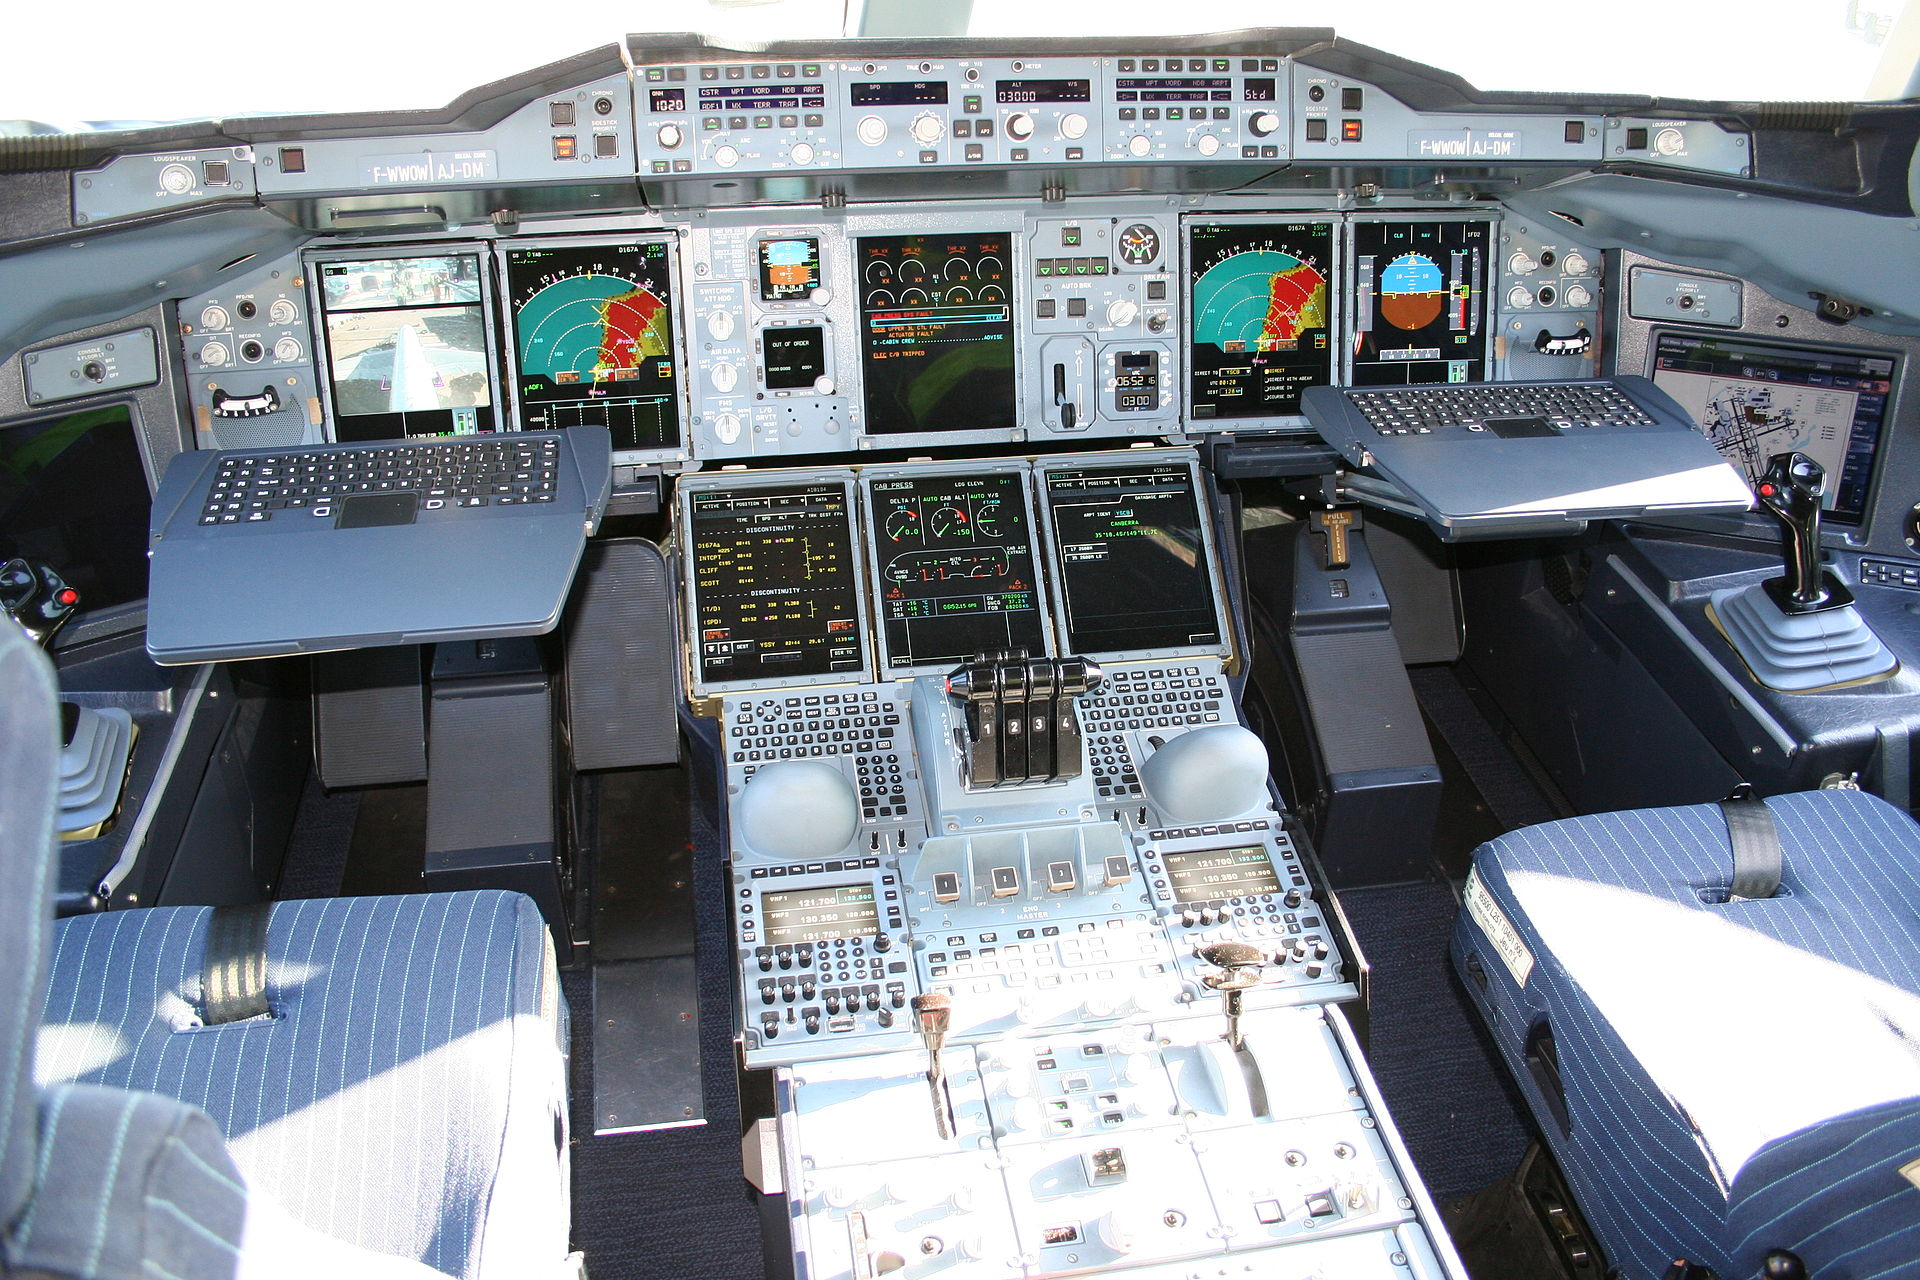
\includegraphics[width=.2\textwidth]{images/cokpit}};
		
		\node[](gr) at ($(coc) + (0pt, 130pt)$) {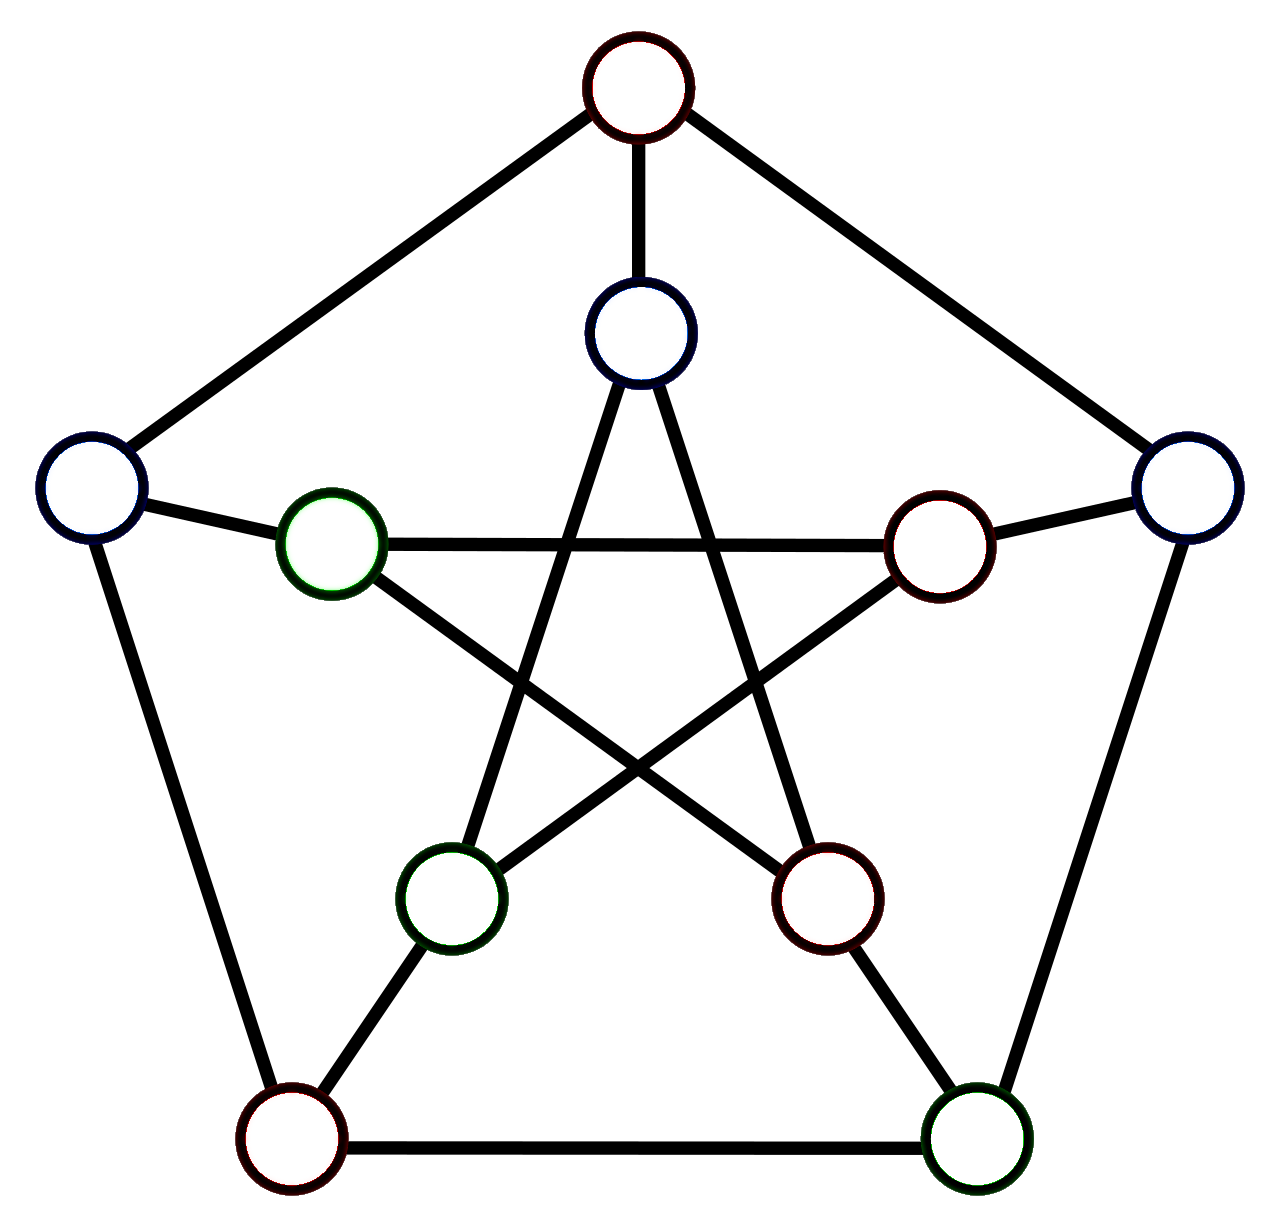
\includegraphics[width=.2\textwidth]{images/graphcoloring2}};
		
	%	\node[opacity=0, onslide={<2>,opacity=1}](gr) at ($(coc) + (0pt, 130pt)$) {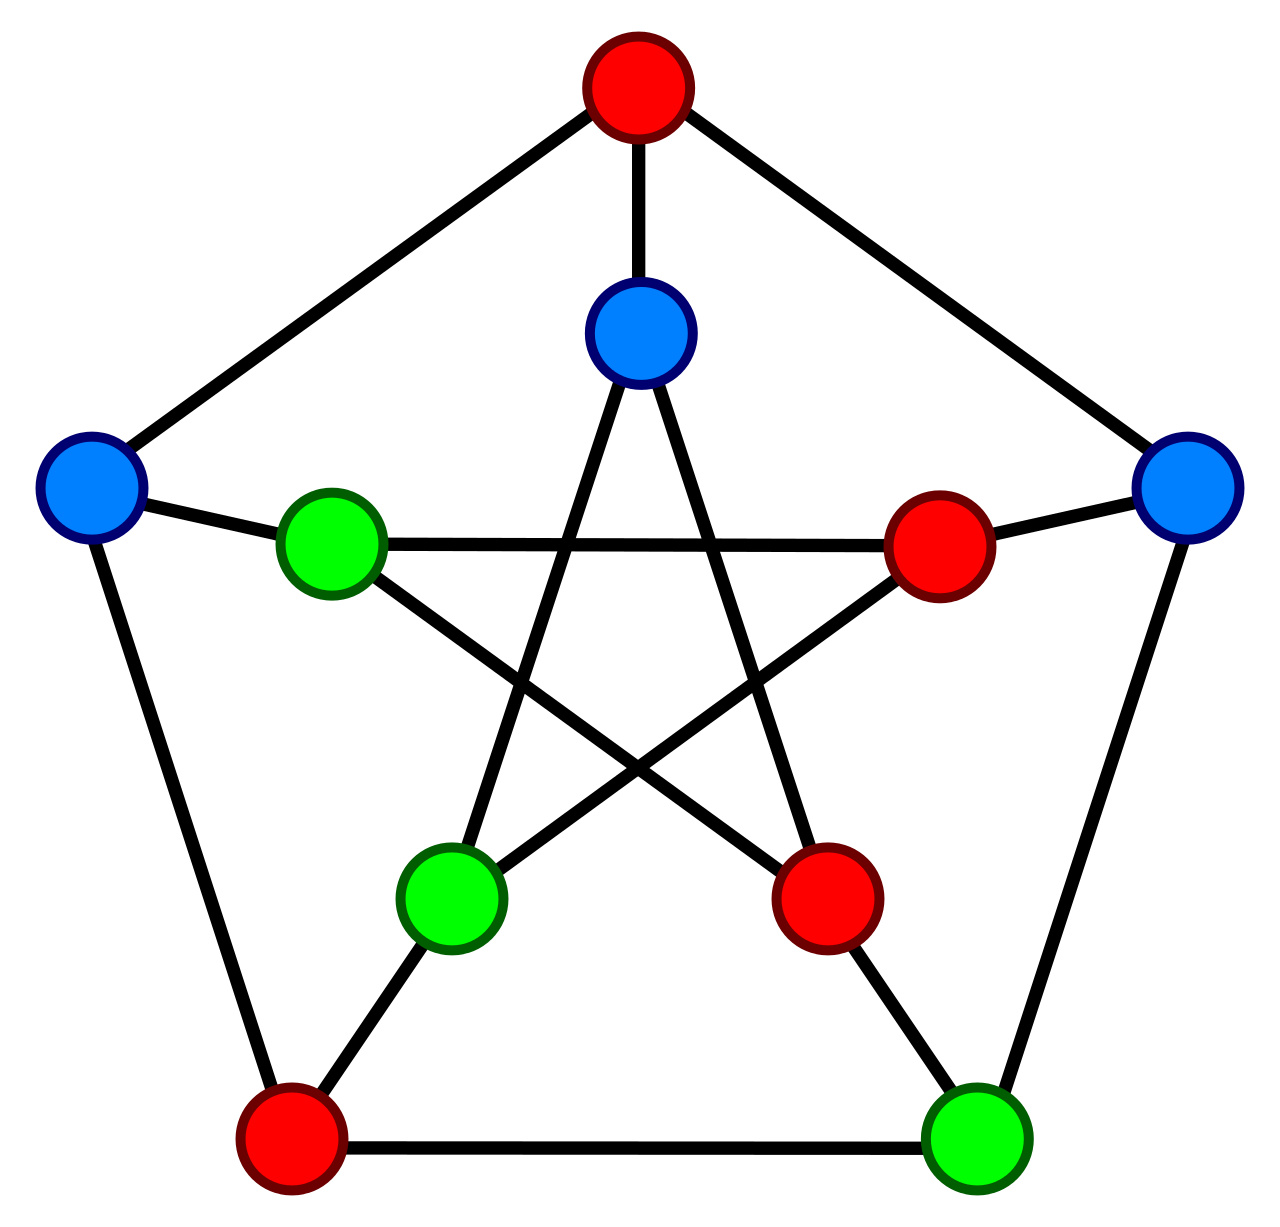
\includegraphics[width=.2\textwidth]{images/graphcoloring}};
		
		
		\node[](c) at ($(coc) + (0pt, 60pt)$) {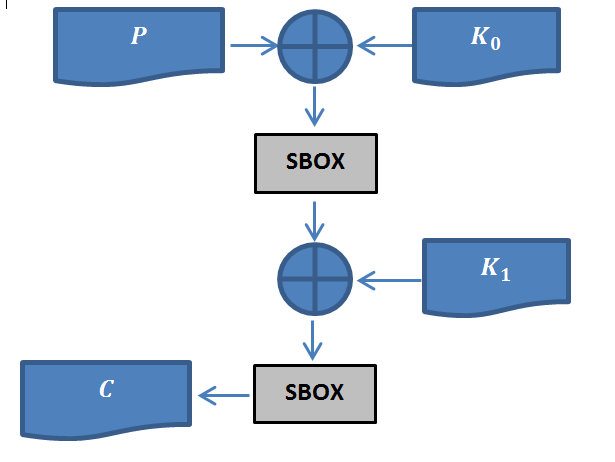
\includegraphics[width=.2\textwidth]{images/crypto}};		
		\node[](p) at ($(coc) + (0pt, -60pt)$) {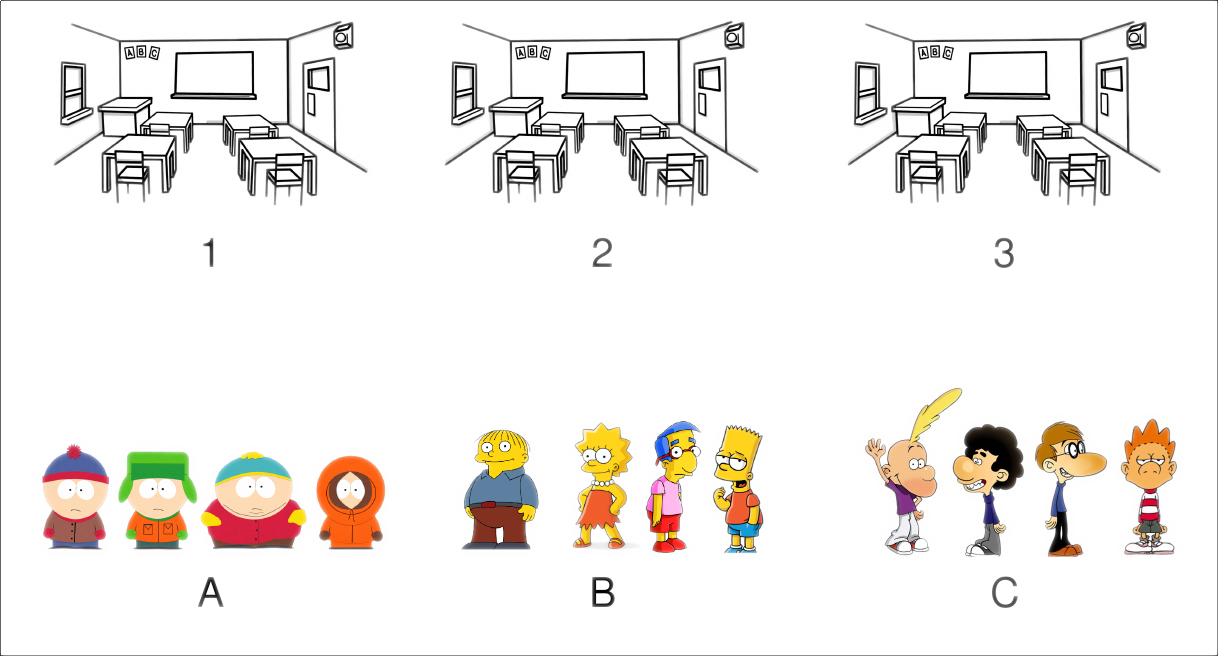
\includegraphics[width=.25\textwidth]{images/plan2}};
		
	   	\node[square, fill=black!20, minimum height=2cm, minimum width=2cm,align=center] (sat) at ($(coc) + (120pt, 40pt)$) {Boolean \\ SATisfiability};
		%\node[square, minimum height=2cm, minimum width=2cm] (sol) at ($(sat) + (100pt, 0pt)$) {Solution};
		
		
		\node[align=center] at ($(coc) + (-100pt, 0pt)$) {Hardware and sofware\\ verification};
		\node at ($(gr) + (-100pt, 0pt)$) {Graph coloring};
		\node[align=center] at ($(c) + (-100pt, 0pt)$) {Cryptanalysis};
		\node[align=center] at ($(p) + (-100pt, 0pt)$) {Planning};
				
		\draw[arr] (coc)  -- (sat);
		\draw[arr] (gr)  to [bend left=30] (sat);
		\draw[arr] (c)  -- (sat);		
		\draw[arr] (p)  to [bend right=30] (sat);
		
%		\draw[arr] (sat)  -- (sol);
		
	\end{tikzpicture}
\end{frame}




%% ----------------------------------------------------------------------------
%\begin{frame}
% %Tackling the explosion in the static symmetry breaking approach
% %Taking the maximum benefits from static and dynamic approaches
%\frametitle{Outline}
%\begin{enumerate}
%	\item \textcolor{UPMCEngagementBlueB}{SAT overview}
%	\begin{itemize}
%		\item[] SAT basics
%		\item[] SAT and symmetries
%	\end{itemize}
%\vspace{5pt}
%	\item \textcolor{UPMCEngagementBlueB}{Existing approaches}
%	\begin{itemize}
%		\item[] \phantom{Static symmetry breaking}
%		\item[] \phantom{Dynamic symmetry breaking}
%	\end{itemize}
%\vspace{5pt}
%	\item \textcolor{UPMCEngagementBlueB}{Contribution and results}
%	\begin{itemize}
%		\item[] \phantom{CDCL [Sym]}
%		\item[] \phantom{Combination of different approaches}
%	\end{itemize}
%\end{enumerate}
%\end{frame}
%% ----------------------------------------------------------------------------


\begin{frame}

\tikzstyle{every picture}+=[remember picture]
\frametitle{SAT: an example (1/2)}
\everymath{\displaystyle}
\centering


\begin{tabular}{ccc}
	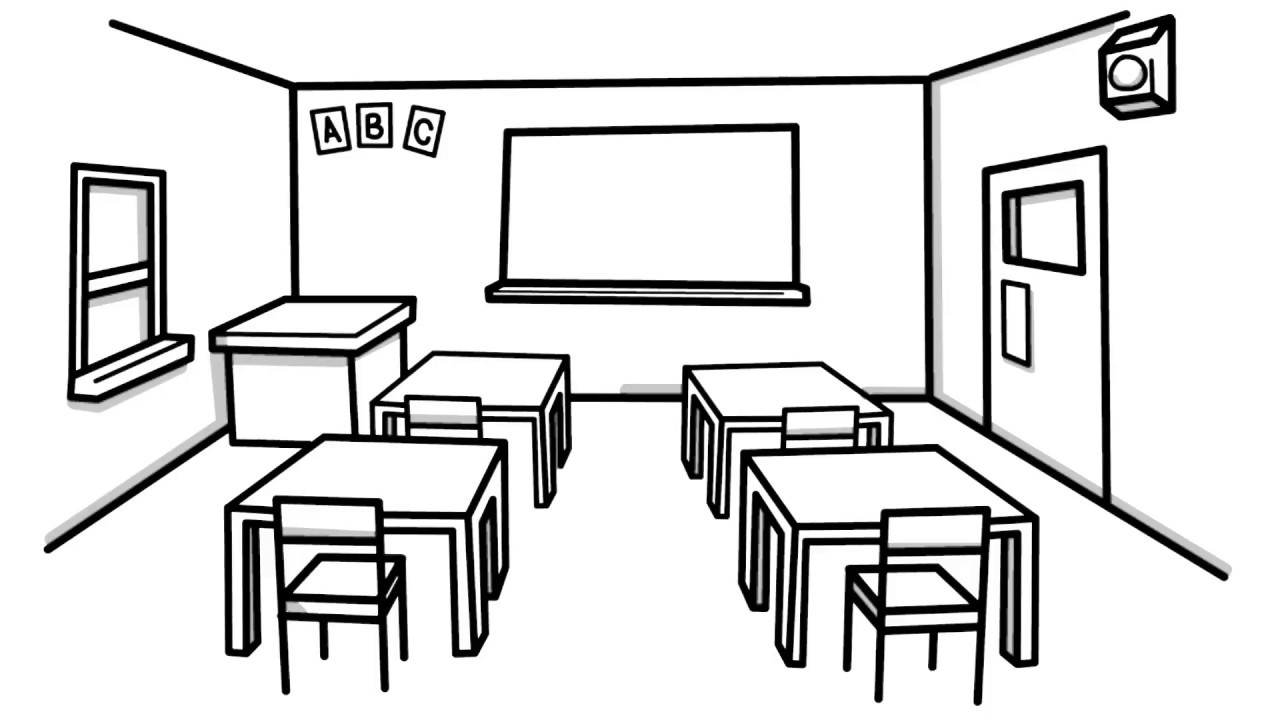
\includegraphics[scale=0.07]{images/room} & 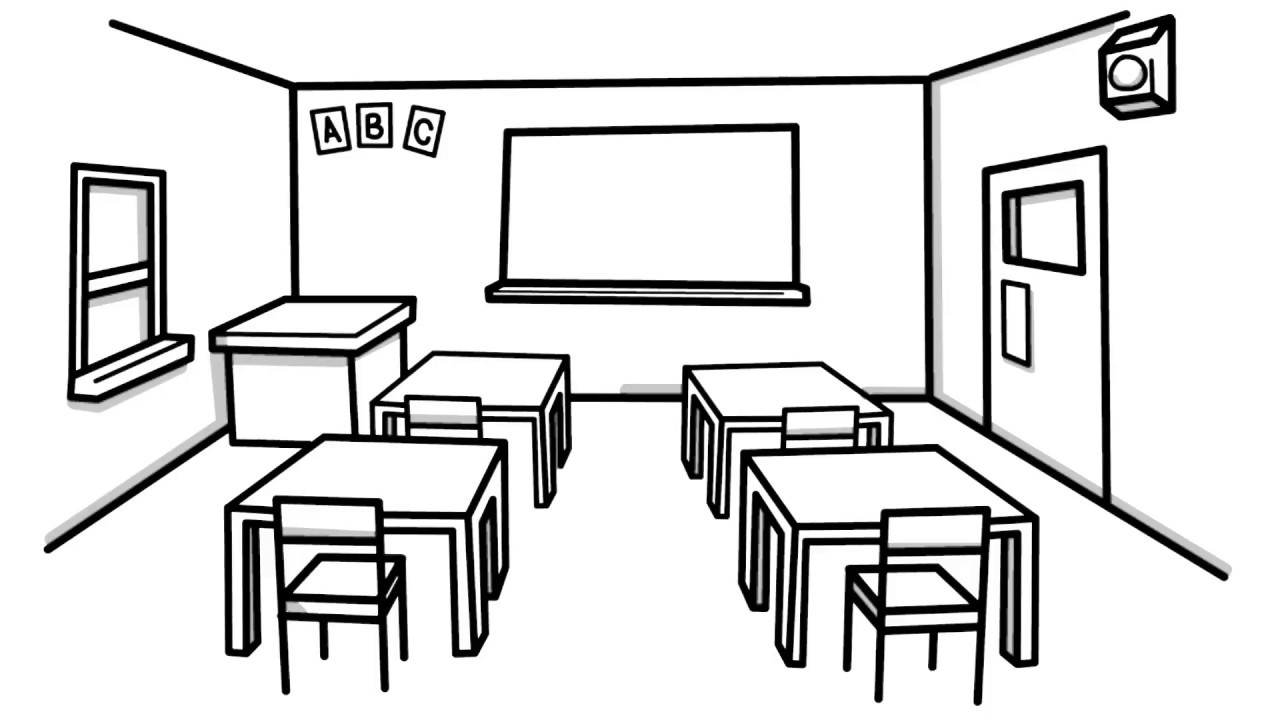
\includegraphics[scale=0.07]{images/room}& 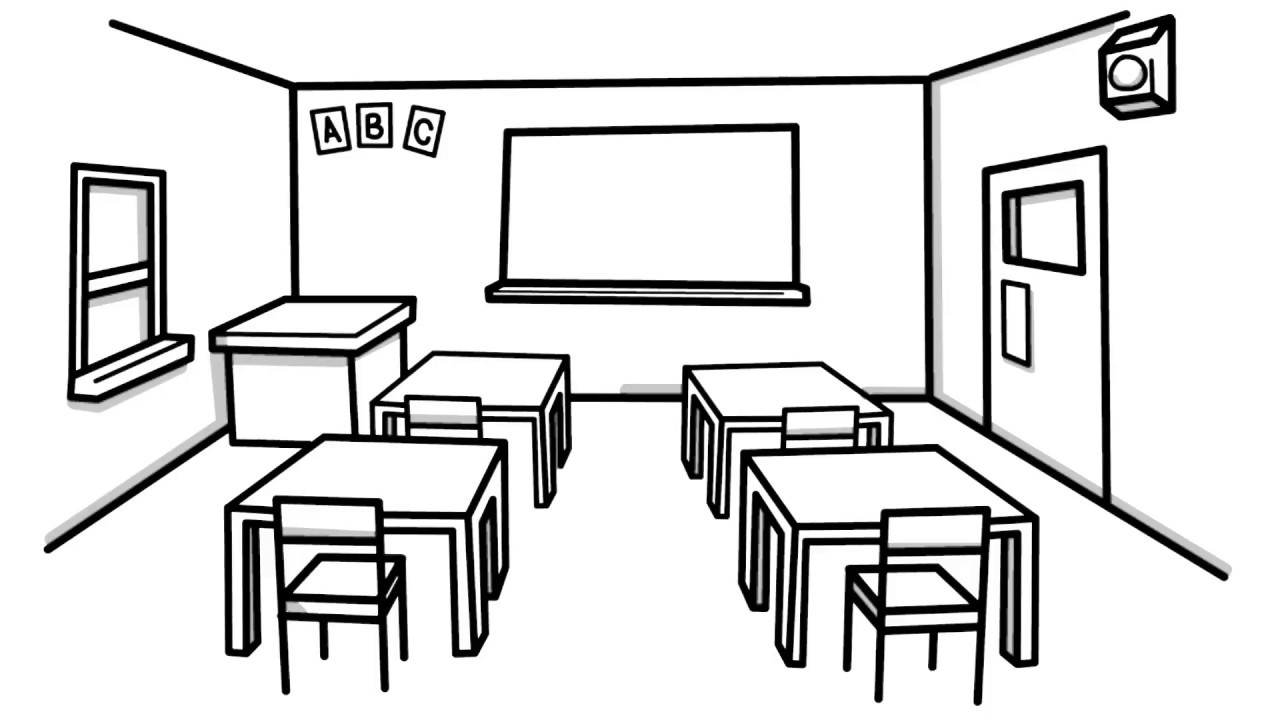
\includegraphics[scale=0.07]{images/room}\\
	\tikz[baseline]{\node[anchor=base] (t1){1};} & \tikz[baseline]{\node[anchor=base] (t2){2};} & \tikz[baseline]{\node[anchor=base] (t3){3};}\\
	 & & \\
	\tikz[baseline]{\node[anchor=base] (s1){};} & \tikz[baseline]{\node[anchor=base] (s2){};} & \tikz[baseline]{\node[anchor=base] (s3){};}\\
	
\includegraphics[scale=0.1]{images/south} & 
\includegraphics[scale=0.1]{images/simpson} & 
\includegraphics[scale=0.09]{images/titeuf}\\
	A                                         & B                                           & C\\
\end{tabular}


\begin{tikzpicture}[overlay]
\tikzstyle{line} = [<-, line width=0.5mm];
\visible<2->{
\path[line] (t1) edge  (s1.south);
\path[line] (t2) edge  (s2.south);
\path[line] (t3) edge  (s3.south);
}
\visible<3->{
\path[line, color=green] (t2.south west) edge  (s1.south);
\path[line, color=green] (t3.south west) edge  (s2.south);
\path[line, color=green] (t1.south west) edge  (s3.south);
}
\visible<4>{
\path[line, color=red] (t1) edge  (s2.south);
\path[line, color=red] (t2) edge  (s1.south);
\path[line, color=red] (t3) edge  (s3.south);

\path[line, color=orange] (t1) edge  (s1.south);
\path[line, color=orange] (t2) edge  (s3.south);
\path[line, color=orange] (t3) edge  (s2.south);

\path[line, color=blue] (t1) edge  (s3.south);
\path[line, color=blue] (t2) edge  (s2.south);
\path[line, color=blue] (t3) edge  (s1.south);


\path[line, color=purple] (t1.south west) edge  (s2.south);
\path[line, color=purple] (t2.south east) edge  (s3.south);
\path[line, color=purple] (t3.south west) edge  (s1.south);
}
\end{tikzpicture}

\vfill
Is it possible to attribute each group to a unique classroom?\\
\begin{center}
	\visible<2->{YES!  \texttt{SAT}isfiable  $\enspace \alpha = \{(A,1), (B,2), (C, 3)\}$\\ }
	\visible<3->{Many solutions $\alpha' = \{(A,2), (B,3), (C, 1)\}$}\\
		 \visible<4->{$\vdots$}
\end{center}


\end{frame}



\begin{frame}
\tikzstyle{every picture}+=[remember picture]
\frametitle{SAT: an example (2/2)}
\everymath{\displaystyle}
\centering

\begin{tabular}{cc}
	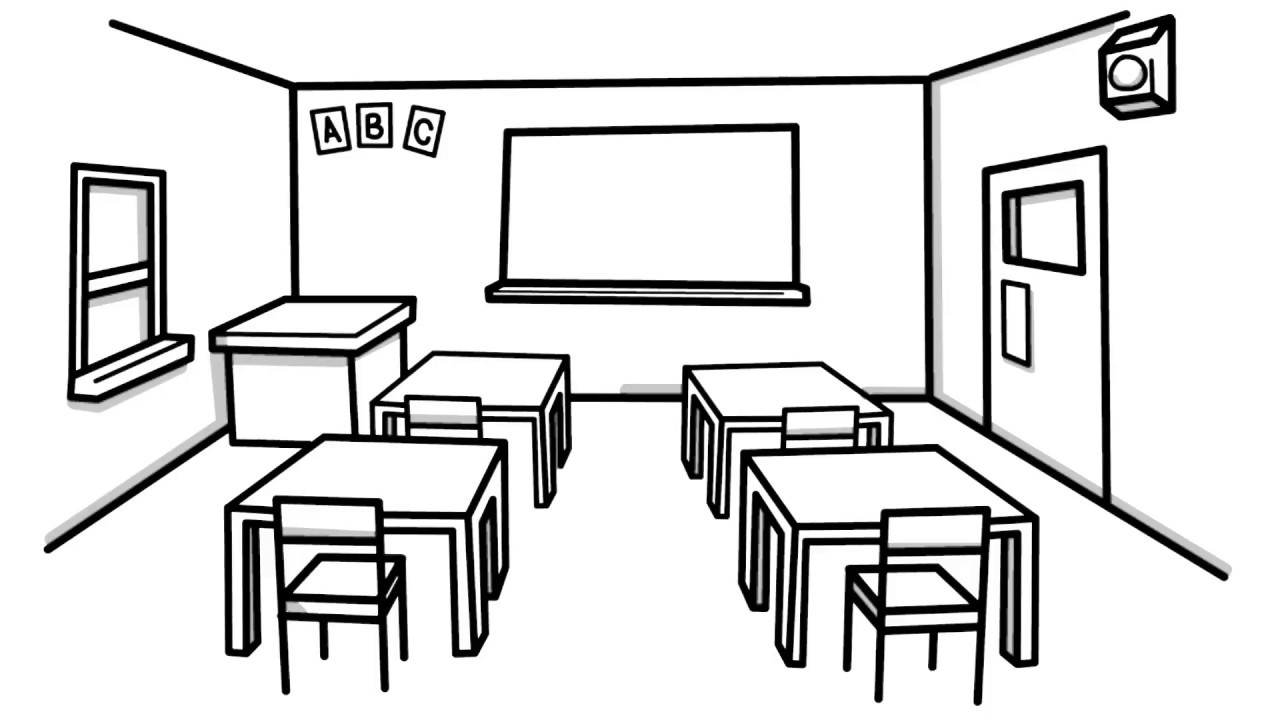
\includegraphics[scale=0.07]{images/room} & 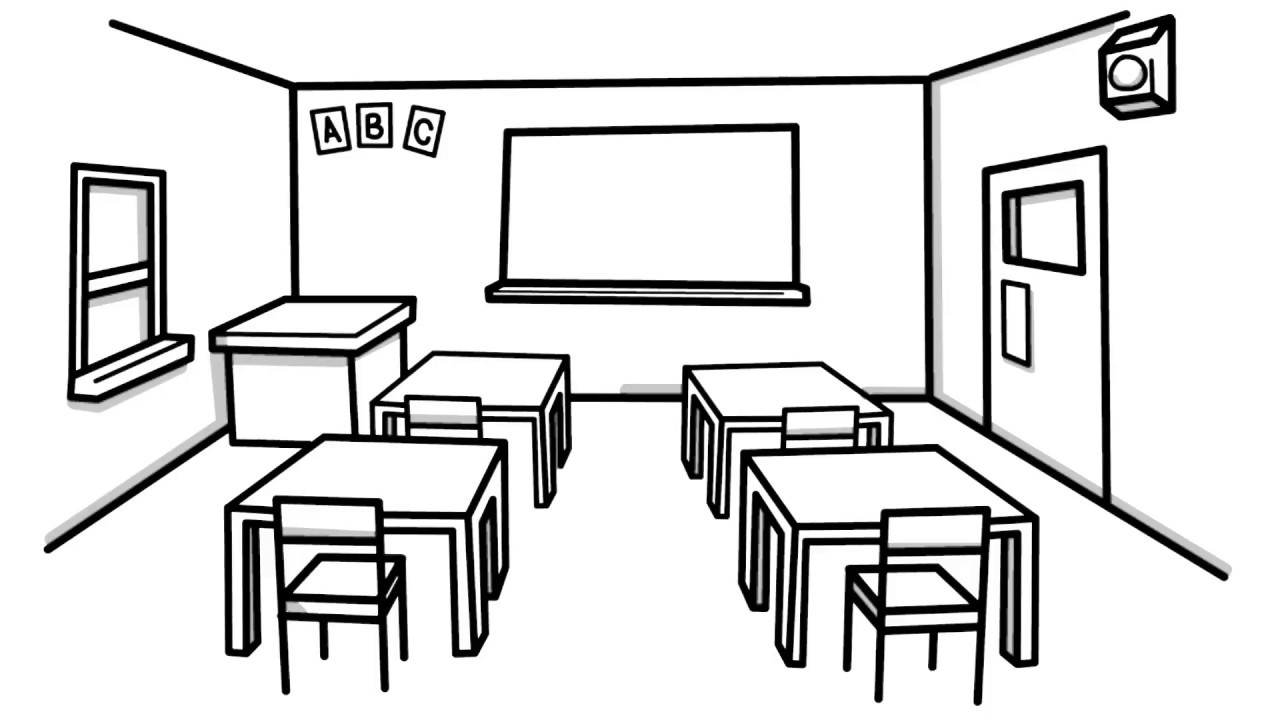
\includegraphics[scale=0.07]{images/room}\\
	\tikz[baseline]{\node[anchor=base] (r1){1};} & \tikz[baseline]{\node[anchor=base] (r2){2};}\\
\end{tabular}


\begin{tabular}{ccc}
	\tikz[baseline]{\node[anchor=base] (g1){};} & \tikz[baseline]{\node[anchor=base] (g2){};} & \tikz[baseline]{\node[anchor=base] (g3){};}\\
	
\includegraphics[scale=0.1]{images/south} & 
\includegraphics[scale=0.1]{images/simpson} & 
\includegraphics[scale=0.09]{images/titeuf}\\
	A                                        & B                                           & C\\
\end{tabular}


\vfill
Is it possible to attribute each group to a unique classroom?
\begin{center}
	\visible<2->{No! \texttt{UNSAT}isfiable}

\end{center}

\end{frame}
%% ----------------------------------------------------------------------------

\begin{frame}
\frametitle{From high level problem to the solution through SAT solving}
\vspace{1em}
\centering
\begin{tikzpicture}
\tikzstyle{box} = [draw, minimum width=3.5cm, thick]
\tikzstyle{result} = [draw, minimum width=2.5cm, minimum height=1cm]

\node[box,result] (hlp) {High level problem};
\node[box, opacity=0, thick,onslide={<2>,opacity=1}] (input) at ($(hlp) + (0pt, -70pt)$){Logic formula};


\node[box, line width=0.4mm, minimum width=10cm,minimum height=4.5cm] (boit) at (0pt, -90pt){};
%\node<2->[draw, ellipse] (cnf) at ($(input) + (0pt, -10pt)$) {\scriptsize CNF};

%\node[rounded,minimum width=3.5cm, minimum height=1cm] (solver) at ($(input) + (0pt, -40pt)$) {SAT solver};
%\node[box,result,align=center] (sat) at ($(solver) + (-70pt, -50pt)$) {Satisfiable ($\texttt{SAT}$) \\ + assignment};
%\node[box,result,align=center] (unsat) at ($(solver) + (70pt, -50pt)$) {Unsatisfiable ($\texttt{UNSAT}$) \\ + proof};


\node[box,result,align=center] (sol) at ($(input) + (0pt, -115pt)$) {High level solution};

\draw[->, opacity=0, thick,onslide={<2>,opacity=1}] (hlp) to node[fill=white,yshift=-0.5em]{encoding} (input);

\draw[->, thick, opacity=1, thick,onslide={<2>,opacity=0}] (hlp) -> (boit);

\draw[->, thick] (boit) -> (sol);

%\visible<2->{\draw[->, thick] (hlp) -> node [midway, fill=white]{Conjunctive Normal Form (CNF)} (input);}

%\draw[->, thick] (input) -> (solver);
%\draw[->, thick] (solver) ->   (sat);
%\draw[->, thick] (solver) -> (unsat);
%
%\draw[->, thick] (sat) ->   (sol);
%\draw[->, thick] (unsat) -> (sol);

\end{tikzpicture}

\end{frame}

\begin{frame}
\frametitle{Encoding the problem}
	
\vspace{1em}
	
\begin{columns}
	\begin{column}{0.1\textwidth}
		\small
		$ \overbrace{(A,1)}^{x_1} \overbrace{(A,2)}^{x_2} \overbrace{(A,3)}^{x_3}$\\
		\visible<2->{
		$(B,1) (B,2) (B,3)$\\
		$(C,1) (C,2) (C,3)$\\
	}
		\vspace{1em}
		\visible<3->{
		$ \neg (A,1)  \neg (B,1)$\\
		$ \neg (A,1)  \neg (C,1)$\\
		$ \neg (B,1)  \neg (C,1)$\\
		}
		\vspace{1em}
		\visible<4->{
		$ \neg (A,2)  \neg (B,2)$\\
		$ \neg (A,2)  \neg (C,2)$\\
		$ \neg (B,2)  \neg (C,2)$\\
		}
		\vspace{1em}
		\visible<4->{
		$ \neg (A,3)  \neg (B,3)$\\
		$ \neg (A,3)  \neg (C,3)$\\
		$ \neg (B,3)  \neg (C,3)$\\
		}
	\end{column}
	\begin{column}{0.2\textwidth}  %%<--- here
		\small
		$(x_1 \lor  x_2 \lor x_3) \enspace \land$\\
			\visible<2->{
		$(x_4 \lor  x_5 \lor x_6) \enspace \land$\\
		$(x_7 \lor  x_8 \lor x_9) \enspace \land$\\
	}
		\vspace{1em}
		\visible<3->{
		$(\neg x_1 \lor  \neg x_4) \enspace \land$\\
		$(\neg x_1 \lor  \neg x_7) \enspace \land$\\
		$(\neg x_4 \lor  \neg x_7) \enspace \land$\\
	}

		\vspace{1em}
		\visible<4->{
		$(\neg x_2 \lor  \neg x_5) \enspace \land$\\
		$(\neg x_2 \lor  \neg x_8) \enspace \land$\\
		$(\neg x_5 \lor  \neg x_8) \enspace \land$\\
	}
		\vspace{1em}
		\visible<4->{
		$(\neg x_3 \lor  \neg x_6) \enspace \land$\\
		$(\neg x_3 \lor  \neg x_9) \enspace \land$\\
		$(\neg x_6 \lor  \neg x_9) \enspace $\\
	}
	\end{column}
\end{columns}

\begin{tikzpicture}[overlay]
	\node[rounded, thick, minimum width=2cm, minimum height=0.5cm,opacity=0,onslide={<5->,opacity=1}] (c) at (208pt, 176pt) {};
	\node[,opacity=0,onslide={<5->,opacity=1}] (ct) at ($(c) + (+90pt, 10pt)$)  {Clause};
	\draw [->,thick,opacity=0,onslide={<5->,opacity=1}] (ct.west) to [bend right=30] (c);
	
	\node[rounded, thick, minimum width=3cm, minimum height=6.5cm,opacity=0,onslide={<6->,opacity=1}](f) at (210pt, 93pt) {};
	\node[,opacity=0,onslide={<6->,opacity=1},align=center] (ft) at ($(f) + (+90pt, 0pt)$) {Conjunctive\\ Normal\\ Form (CNF)};
	\draw [->,thick,opacity=0,onslide={<6->,opacity=1}] (ft.west) to [bend right=0] (f);
	
	\node[](p) at (20pt, 88pt) {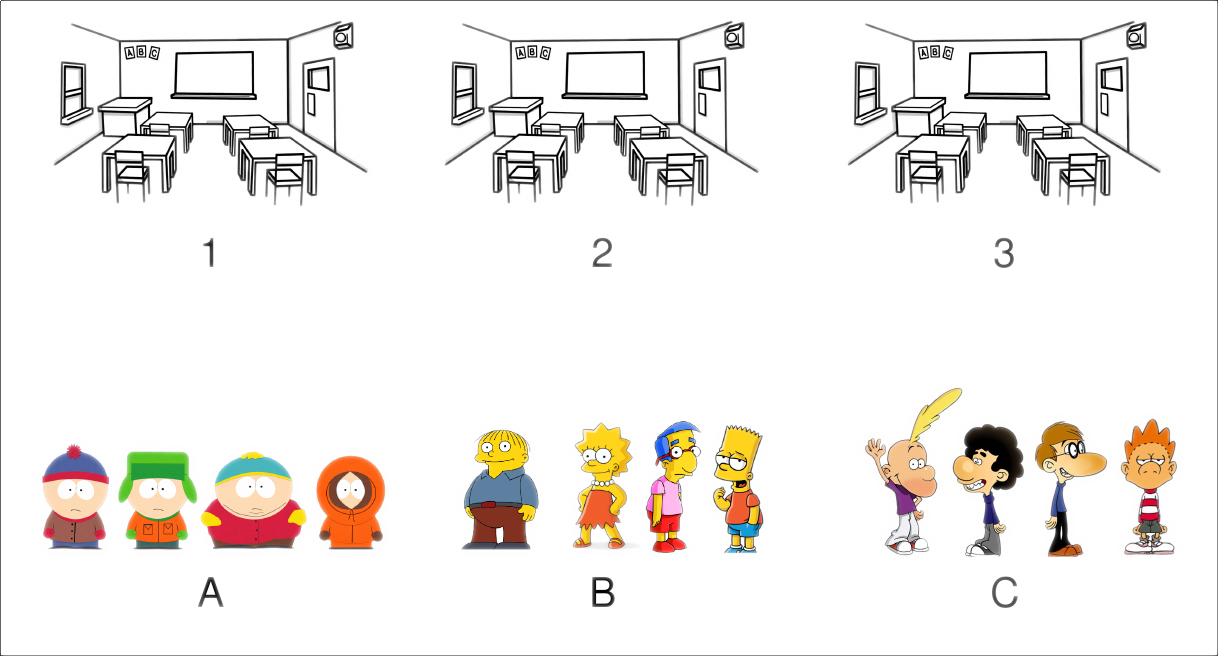
\includegraphics[width=.25\textwidth]{images/plan2}};
	
	\draw[thick] (5.5, 0) -- (5.5, 6);
\end{tikzpicture}

%\visible<3>{
%	\begin{center}
%		Conjunctive Normal Form (CNF)
%	\end{center}
%	}
\vfill
\visible<6>{
Any Boolean formula can be transformed into CNF in polynomial time
}
\visible<7->{
	Clause represented as a set:
	\begin{center}
		$(x_1 \lor x_2 \lor x_3) \rightarrow \{x_1, x_2, x_3\}$
	\end{center}
}
\end{frame}




%% ----------------------------------------------------------------------------

%
%%% ----------------------------------------------------------------------------
%\begin{frame}
%\frametitle{Encoding the problem}
%\begin{columns}
%	\begin{column}{0.1\textwidth}
%		\small
%		$(A,1) (A,2) $\\
%		$(B,1) (B,2) $\\
%		$(C,1) (C,2) $\\
%		\vspace{1em}
%		$ \neg (A,1)  \neg (B,1)$\\
%		$ \neg (A,1)  \neg (C,1)$\\
%		$ \neg (B,1)  \neg (C,1)$\\
%		\vspace{1em}
%		$ \neg (A,2)  \neg (B,2)$\\
%		$ \neg (A,2)  \neg (C,2)$\\
%		$ \neg (B,2)  \neg (C,2)$\\
%	\end{column}
%	\begin{column}{0.2\textwidth}  %%<--- here
%		\small
%		$ x_1 \lor  x_2 $ \\
%		$x_3 \lor  x_4  $ \\
%		$x_5 \lor  x_6 $ \\
%		\vspace{1em}
%		$ \neg x_1 \lor  \neg x_3 $ \\
%		$ \neg x_1 \lor  \neg x_5 $ \\
%		$ \neg x_3 \lor  \neg x_5 $ \\
%		\vspace{1em}
%		$\neg x_2 \lor  \neg x_4 $ \\
%		$ \neg x_2 \lor  \neg x_6 $ \\
%		$ \neg x_4 \lor  \neg x_6 $ \\
%	\end{column}
%\end{columns}
%
%%$\omega_1 = x_1 \lor  x_2 \lor x_3 $ \\
%%$\omega_2 = x_4 \lor  x_5 \lor x_6 $ \\
%%$\omega_3 = x_7 \lor  x_8 \lor x_9 $ \\
%%\vspace{1em}
%%$\omega_4 = \neg x_1 \lor  \neg x_4 $ \\
%%$\omega_5 = \neg x_1 \lor  \neg x_7 $ \\
%%$\omega_6 = \neg x_4 \lor  \neg x_7 $ \\
%%\vspace{1em}
%%$\omega_7 = \neg x_2 \lor  \neg x_5 $ \\
%%$\omega_8 = \neg x_2 \lor  \neg x_8 $ \\
%%$\omega_9 = \neg x_5 \lor  \neg x_8 $ \\
%%\vspace{1em}
%%$\omega_{10} = \neg x_3 \lor  \neg x_6 $ \\
%%$\omega_{11} = \neg x_3 \lor  \neg x_9 $ \\
%%$\omega_{12} = \neg x_6 \lor  \neg x_9 $ \\
%\end{frame}
%% ----------------------------------------------------------------------------

\begin{frame}
\frametitle{From high level problem to the solution through SAT solving}
\vspace{1em}
\centering
\begin{tikzpicture}
\tikzstyle{box} = [draw, minimum width=3.5cm, thick]
\tikzstyle{result} = [draw, minimum width=2.5cm, minimum height=1cm]

\node[box,result] (hlp) {High level problem};
\node[box] (input) at ($(hlp) + (0pt, -40pt)$){Logic formula};


%\node[box, line width=0.4mm, minimum width=10cm,minimum height=4.75cm]  at (0pt, -85pt){};
%\node<2->[draw, ellipse] (cnf) at ($(input) + (0pt, -10pt)$) {\scriptsize CNF};

\node[rounded,minimum width=3.5cm, minimum height=1cm] (solver) at ($(input) + (0pt, -40pt)$) {SAT solver};

\node[rounded,minimum width=3.5cm, minimum height=1cm,opacity=0,draw=olive,line width=0.7mm,onslide={<2>,opacity=1}] (so) at ($(input) + (0pt, -40pt)$) {SAT solver};
\node[box,result,align=center] (sat) at ($(solver) + (-70pt, -50pt)$) {Satisfiable ($\texttt{SAT}$) \\ + assignment};
\node[box,result,align=center] (unsat) at ($(solver) + (70pt, -50pt)$) {Unsatisfiable ($\texttt{UNSAT}$) \\ + proof};

\node[box, line width=0.4mm, minimum width=10cm,minimum height=4.75cm] (boit) at (0pt, -90pt){};
\node[box,result,align=center] (sol) at ($(solver) + (0pt, -100pt)$) {High level solution};

\draw[->, thick] (hlp) -> (input);
%\visible<2->{\draw[->, thick] (hlp) -> node [midway, fill=white]{Conjunctive Normal Form (CNF)} (input);}
\draw[->, thick] (input) -> (solver);
\draw[->, thick] (solver) ->   (sat);
\draw[->, thick] (solver) -> (unsat);

\draw[->, thick] (sat) ->   (sol);
\draw[->, thick] (unsat) -> (sol);

\end{tikzpicture}

\end{frame}

%% ----------------------------------------------------------------------------

\begin{frame}
\frametitle{SAT Solving}

	Solving SAT formula is known to be \textbf{NP-complete}~\cite{cook1971complexity}
	\vfill
	\visible<1->{
			Good performance in practice:
	\begin{itemize}
		\item Handle large problem (million variables and clauses)
		\item International SAT competition each year on academic and industrial problems
	\end{itemize}
}
\vfill
\visible<2->{
	Enumerative algorithms:
	\begin{itemize}
		\item Davis, Putnam, Logemann, and Loveland (DPLL)~\cite{dpll_62}
		\begin{itemize}
			\item Boolean Constraint Propagation (BCP)
		\end{itemize}
	
		\item \textbf{Conflict Driven Clause Learning} (CDCL)~\cite{marques1999grasp}
		\begin{itemize}
			\item Derived from DPLL
			\item Clause learning
		\end{itemize}
	\end{itemize}
}
\end{frame}


\begin{frame}
	\frametitle{CDCL in detail}
	\centering
	\begin{tikzpicture}[scale=0.9,every node/.style={scale=0.5,fill=white, font=\sffamily}, align=center]
	% Specification of nodes (position, etc.)
	\tikzset{%
		>={Latex[width=2mm,length=2mm]},
		% Specifications for style of nodes:
		base/.style = {rectangle, rounded corners, draw=black,opacity=0,
			minimum width=2cm, minimum height=1cm,
			text centered, font=\sffamily},
		question/.style = {base, diamond, fill=blue!15},
		question/.style = {base, diamond, fill=blue!15},
		unsat/.style = {base, fill=red!30,minimum width=3cm},
		sat/.style = {base, fill=green!30,minimum width=3cm},
		process/.style = {base, minimum width=2.5cm, fill=orange!25,
			font=\ttfamily},
		processcurr/.style = {process, thick, line width=0.7mm, draw=purple!80 },
		focus/.style = {opacity=1},
		questioncurr/.style = {question,line width=0.7mm, draw=purple!80},
		line/.style = {->, thick,opacity=0},
		linecurr/.style = {line, line width=0.7mm, draw=purple!80},
	}
	
	\node (isfin) [question,onslide={<8->,focus}] {All clauses\\ satisfied?};
	\node (dec)     [process,onslide={<1->,focus}] at ($(isfin) + (0pt, -50pt)$)    {Choose decision};
	\node (sdec)    at ($(dec) + (180pt, 0pt)$)          {Start};
	\node (idec) [left = of isfin]  {};
	\node (prop)    [process,onslide={<2->,focus}] at ($(dec) + (0pt, -30pt)$)      {Unit propagation\\(BCP)};
	
	
	\node (conf)    [question,onslide={<3->,focus}] at ($(prop) + (0pt, -40pt)$){ Is conflict?};
	\node (confanalyse) [process,onslide={<4->,focus}] at ($(conf) + (0pt, -60pt)$) {Conflict analysis};
	\node (learn) [process,onslide={<7->,focus}] at ($(prop) + (90pt, 0)$) {Learn conflict clause\\ and backjump};
	\node (isend) [question,onslide={<5->,focus}] at ($(confanalyse) + (90pt, 0)$) {is level\\zero?};
	
	\node (end) [unsat,double=black!10,double distance=0.5mm,onslide={<6->,focus}] at ($(isend) + (90pt, 0)$) {$unsatiasfiable$};
	
	\node (ends) [sat,double=black!10,double distance=0.5mm,,onslide={<10->,focus}] at ($(isfin) + (+180pt, 0)$){$satisfiable$};
	
	
	\draw[line,onslide={<1->,focus}]     (sdec) -- (dec);
	\draw[line,onslide={<2->,focus}]     (dec) -- (prop);
	\draw[line,onslide={<3->,focus}]     (prop) -- (conf);
	\draw[line,onslide={<8->,focus}]     (conf) -| node [yshift=4.5 cm] {no}(idec.center) -- (isfin);
	
	\draw[line,onslide={<4->,focus}]     (conf) -- node {yes} (confanalyse);
	\draw[line,onslide={<5->,focus}]     (confanalyse) --(isend);
	\draw[line,onslide={<6->,focus}]     (isend) -- node {yes}(end);
	\draw[line,onslide={<7->,focus}]     (learn) -- (prop);
			
	\draw[line,onslide={<9->,focus}]     (isfin) -- node {no}(dec);


	\draw[line,onslide={<10->,focus}]     (isfin) -- node {yes}(ends);

	\draw[line,onslide={<7->,focus}]     (isend) -- node [thick] {no}(learn);
	

	
	\end{tikzpicture}
\end{frame}
%% ----------------------------------------------------------------------------
%\begin{frame}
%\frametitle{Conflict Driven Clause Learning (CDCL)}
%
%\centering
%
%\begin{tikzpicture}[scale=1,every node/.style={scale=0.6,fill=white, font=\sffamily}, align=center]
%	% Specification of nodes (position, etc.)
%	\tikzset{%
%		>={Latex[width=2mm,length=2mm]},
%		% Specifications for style of nodes:
%		base/.style = {rectangle, rounded corners, draw=black,
%			minimum width=2cm, minimum height=1cm,
%			text centered, font=\sffamily},
%		question/.style = {base, diamond, fill=blue!15},
%		question/.style = {base, diamond, fill=blue!15},
%		unsat/.style = {base, fill=red!30,minimum width=3cm},
%		sat/.style = {base, fill=green!30,minimum width=3cm},
%		process/.style = {base, minimum width=2.5cm, fill=orange!25,
%			font=\ttfamily},
%		processcurr/.style = {process, thick, line width=0.7mm, draw=purple!80 },
%		questioncurr/.style = {question,line width=0.7mm, draw=purple!80},
%		line/.style = {->, thick },
%		linecurr/.style = {line, line width=0.7mm, draw=purple!80},
%	}
%	\node (isfin) [question] {All vars\\ assign?};
%	\node (dec)     [process, below = of isfin]          {Choose decision var};
%	\node (sdec)     [right = of dec]          {};
%	\node (idec) [left = of isfin]  {};
%	\node (prop)    [process] at ($(dec) + (0pt, -30pt)$)          {Unit Propagation};
%	\node (conf)    [question] at ($(prop) + (0pt, -50pt)$){ Is Conflict?};
%	\node (confanalyse) [process, below = of conf] {Conflict Analysis};
%	\node (learn) [process] at ($(prop) + (90pt, 0)$) {Learn conflict clause};
%	\node (isend) [question] at ($(confanalyse) + (90pt, 0)$) {is level\\zero?};
%	\node (end) [unsat] at ($(isend) + (90pt, 0)$) {$unsatiasfiable$};
%	\node (ends) [sat] at ($(isfin.north east) + (+90pt, 0)$){$satisfiable$};
%
%	\draw[line]     (sdec) -- (dec);
%	\draw[line]     (dec) -- (prop);
%	\draw[line]     (prop) -- (conf);
%	\draw[line]     (conf) -| node [yshift=4.5 cm] {no}(idec.center) -- (isfin);
%	\draw[line]     (conf) -- node {yes} (confanalyse);
%	\draw[line]     (isfin) -- node {no}(dec);
%	\draw[line]     (confanalyse) --(isend);
%	\draw[line]     (isend) -- node {yes}(end);
%	\draw[line]     (isfin.north east) -- node {yes}(ends);
%	\draw[line]     (learn) -- (prop);
%	\draw[line]     (isend) -- node [] {no}(learn);
%	\end{tikzpicture}
%
%\end{frame}

%% ----------------------------------------------------------------------------


\begin{frame}
\frametitle{CDCL in action}

 \begin{columns}[t]
	\begin{column}[T]{.6\textwidth}
\begin{tikzpicture}[scale=0.8, every node/.style={scale=0.8}]
\newcommand{\x}{2}
\newcommand{\y}{-1.5}

\tikzstyle{decision}=[circle,draw,thick,fill=blue!30,font=\scriptsize,anchor=base, nearly transparent]
\tikzstyle{propagation}=[rectangle, minimum height=.65cm, minimum width=.65cm,draw,thick,fill=blue!30,font=\scriptsize,anchor=base]
\tikzstyle{space}=[regular polygon, regular polygon sides=3, minimum height=1cm, anchor=base,xshift=-0.25cm,yshift=-0.25cm,
draw,thick,fill=blue!30,rotate=0,font=\scriptsize]
\tikzstyle{unsat}=[draw,thick,fill=red, nearly transparent]
\tikzstyle{sat}=[draw,thick,fill=green, nearly transparent]
\tikzstyle{link}=[->,>=latex,rounded corners=5pt,thick, nearly transparent]
\tikzstyle{trlink}=[link,nearly transparent]
\tikzstyle{mid}=[midway,fill=white,nearly transparent,opacity=1, text opacity=1,font=\scriptsize]
\tikzstyle{trmid}=[midway,fill=white,nearly transparent,opacity=1, text opacity=0.3,font=\scriptsize]

% layer 1
\node[decision,onslide={<2-3>,opacity=1},onslide={<5->,propagation,opacity=1}](t) at (0,0) {$x_1$};

% layer 2
\node[decision](l) at (-\x,\y) {$x_2$};
\node[scale=2,opacity=0,onslide={<5->, opacity=1}](lko) at (-\x,\y) {\ko};
\node[decision,onslide={<6-7>,opacity=1},onslide={<9->,propagation,opacity=1}](r) at (\x,\y) {$x_2$};

% layer 3
\node[decision](ll) at (-\x-\x*0.5,2*\y) {$x_3$};
\node[decision](lr) at (-\x+\x*0.5,2*\y) {$x_3$};
\node[decision](rl) at (\x-\x*0.5,2*\y) {$x_3$};
\node[scale=2,opacity=0,onslide={<9->,opacity=1}](rlko) at (\x-\x*0.5,2*\y) {\ko};
\node[decision,onslide={<10->,opacity=1}](rr) at (\x+\x*0.5,2*\y) {$x_3$};

% layer 4
\node[decision](lll) at (-\x-\x*0.5-\x*0.25,3*\y) {$x_4$};
\node[decision](llr) at (-\x-\x*0.5+\x*0.25,3*\y) {$x_4$};
\node[decision](lrl) at (-\x+\x*0.5-\x*0.25,3*\y) {$x_4$};
\node[decision](lrr) at (-\x+\x*0.5+\x*0.25,3*\y) {$x_4$};
\node[decision](rll) at (\x-\x*0.5-\x*0.25,3*\y) {$x_4$};
\node[decision](rlr) at (\x-\x*0.5+\x*0.25,3*\y) {$x_4$};
\node[decision,onslide={<11->,opacity=1,propagation}](rrl) at (\x+\x*0.5-\x*0.25,3*\y) {$x_4$};
%\node[decision](rrr) at (\x+\x*0.5+\x*0.25,3*\y) {$x_4$};

% layer 5
\node[unsat](llll) at (-\x-\x*0.5-\x*0.25-\x*0.125,4*\y) {};
\node[unsat](lllr) at (-\x-\x*0.5-\x*0.25+\x*0.125,4*\y) {};
\node[unsat](llrl) at (-\x-\x*0.5+\x*0.25-\x*0.125,4*\y) {};
\node[unsat](llrr) at (-\x-\x*0.5+\x*0.25+\x*0.125,4*\y) {};
\node[unsat](lrll) at (-\x+\x*0.5-\x*0.25-\x*0.125,4*\y) {};
\node[unsat](lrlr) at (-\x+\x*0.5-\x*0.25+\x*0.125,4*\y) {};
\node[unsat](lrrl) at (-\x+\x*0.5+\x*0.25-\x*0.125,4*\y) {};
\node[unsat](lrrr) at (-\x+\x*0.5+\x*0.25+\x*0.125,4*\y) {};

\node[unsat](rlll) at (\x-\x*0.5-\x*0.25-\x*0.125,4*\y) {};
\node[unsat](rllr) at (\x-\x*0.5-\x*0.25+\x*0.125,4*\y) {};
\node[unsat](rlrl) at (\x-\x*0.5+\x*0.25-\x*0.125,4*\y) {};
\node[unsat](rlrr) at (\x-\x*0.5+\x*0.25+\x*0.125,4*\y) {};
\node[unsat](rrll) at (\x+\x*0.5-\x*0.25-\x*0.125,4*\y) {};
\node[sat,onslide={<11->,opacity=1}](rrlr) at (\x+\x*0.5-\x*0.25+\x*0.125,4*\y) {};
%\node[unsat](rrrl) at (\x+\x*0.5+\x*0.25-\x*0.125,4*\y) {};
%\node[unsat](rrrr) at (\x+\x*0.5+\x*0.25+\x*0.125,4*\y) {};


\draw[link,onslide={<2-3>,opacity=1}] (t) ->  node [trmid, onslide={<2-3>,mid}] {$0$} (l);
\draw[link,onslide={<5->,opacity=1}] (t) -> node [trmid, onslide={<5->,mid}] {$1$} (r);

\draw[link] (l) ->  node [trmid] {$0$} (ll);
\draw[link] (l) -> node [trmid] {$1$} (lr);
\draw[link,onslide={<6-7>,opacity=1}] (r) ->  node [trmid,onslide={<6-7>,mid}] {$0$} (rl);
\draw[link,onslide={<9->,opacity=1}] (r) -> node [trmid,onslide={<9->,mid}] {$1$} (rr);

\draw[link] (ll) -> node [trmid] {$0$} (lll);
\draw[link] (ll) -> node [trmid] {$1$} (llr);
\draw[link] (lr) -> node [trmid] {$0$} (lrl);
\draw[link] (lr) -> node [trmid] {$1$} (lrr);
\draw[link] (rl) -> node [trmid] {$0$} (rll);
\draw[link] (rl) -> node [trmid] {$1$} (rlr);
\draw[link,onslide={<10->,opacity=1}] (rr) -> node [trmid,onslide={<10->,text opacity=1}] {$0$} (rrl);
%	\draw[link] (rr) -> node [trmid] {$1$} (rrr);


\draw[link] (lll) -> node [trmid] {$0$} (llll);
\draw[link] (lll) -> node [trmid] {$1$} (lllr);
\draw[link] (llr) -> node [trmid] {$0$} (llrl);
\draw[link] (llr) -> node [trmid] {$1$} (llrr);
\draw[link] (lrl) -> node [trmid] {$0$} (lrll);
\draw[link] (lrl) -> node [trmid] {$1$} (lrlr);
\draw[link] (lrr) -> node [trmid] {$0$} (lrrl);
\draw[link] (lrr) -> node [trmid] {$1$} (lrrr);
\draw[link] (rll) -> node [trmid] {$0$} (rlll);
\draw[link] (rll) -> node [trmid] {$1$} (rllr);
\draw[link] (rlr) -> node [trmid] {$0$} (rlrl);
\draw[link] (rlr) -> node [trmid] {$1$} (rlrr);
\draw[link] (rrl) -> node [trmid] {$0$} (rrll);
\draw[link,onslide={<11->,opacity=1}] (rrl) -> node [trmid,onslide={<11->,text opacity=1}] {$1$} (rrlr);
%	\draw[link] (rrr) -> node [trmid] {$0$} (rrrl);
%	\draw[link] (rrr) -> node [trmid] {$1$} (rrrr);
\end{tikzpicture}
\end{column}
\begin{column}[T]{.4\textwidth}

	\only<1>{
		\begin{itemize}
			\item[] $\omega_1 = \{x_1, x_2, x_3, x_4\}$
			\item[] $\omega_2 = \{x_1, \neg x_4\}$
			\item[] $\omega_3 = \{x_1, x_4\}$
			\item[] $\omega_4 = \{x_2, \neg x_4\}$
			\item[] $\omega_5 = \{x_2, x_4\}$
			\item[] $\omega_6 = \{x_3, x_4\}$
		\end{itemize}
	}
	\only<2>{
		\begin{itemize}
			\item[] $\omega_1 = \{\textcolor{red}{x_1}, x_2, x_3, x_4\}$
			\item[] $\omega_2 = \{\textcolor{red}{x_1}, \neg x_4\}$
			\item[] $\omega_3 = \{\textcolor{red}{x_1}, x_4\}$
			\item[] $\omega_4 = \{x_2, \neg x_4\}$
			\item[] $\omega_5 = \{x_2, x_4\}$
			\item[] $\omega_6 = \{x_3, x_4\}$
		\end{itemize}
	}
	\only<3>{
		\begin{itemize}
			\item[] $\omega_1 = \{\textcolor{red}{x_1}, x_2, x_3, x_4\}$
			\item[] $\omega_2 = \{\textcolor{red}{x_1}, \textcolor{blue}{\neg x_4}\}$
			\item[] $\omega_3 = \{\textcolor{red}{x_1}, \textcolor{blue}{x_4}\}$
			\item[] $\omega_4 = \{x_2, \neg x_4\}$
			\item[] $\omega_5 = \{x_2, x_4\}$
			\item[] $\omega_6 = \{x_3, x_4\}$
		\end{itemize}
	}

	\only<4>{
		\begin{itemize}
			\item[] $\omega_1 = \{x_1, x_2, x_3, x_4\}$
		\item[] $\omega_2 = \{x_1, \neg x_4\}$
		\item[] $\omega_3 = \{x_1, x_4\}$
		\item[] $\omega_4 = \{x_2, \neg x_4\}$
		\item[] $\omega_5 = \{x_2, x_4\}$
		\item[] $\omega_6 = \{x_3, x_4\}$
		\end{itemize}
	}
	\only<5>{
	\begin{itemize}
		\item[] $\textcolor{green}{\omega_1} = \{\textcolor{green}{x_1}, x_2, x_3,
		x_4\}$
		\item[] $\textcolor{green}{\omega_2} = \{\textcolor{green}{x_1}, \neg x_4
		\}$
		\item[] $\textcolor{green}{\omega_3} = \{\textcolor{green}{x_1}, x_4\}$
		\item[] $\omega_4 = \{x_2, \neg x_4\}$
		\item[] $\omega_5 = \{x_2, x_4\}$
		\item[] $\omega_6 = \{x_3, x_4\}$
	\end{itemize}
}
	\only<6>{
		\begin{itemize}
			\item[] $\textcolor{green}{\omega_1} = \{\textcolor{green}{x_1},
			\textcolor{red}{x_2}, x_3, x_4\}$
			\item[] $\textcolor{green}{\omega_2} = \{\textcolor{green}{x_1}, \neg x_4
			\}$
			\item[] $\textcolor{green}{\omega_3} = \{\textcolor{green}{x_1}, x_4\}$
			\item[] $\omega_4 = \{\textcolor{red}{x_2}, \neg x_4\}$
			\item[] $\omega_5 = \{\textcolor{red}{x_2}, x_4\}$
			\item[] $\omega_6 = \{x_3, x_4\}$
		\end{itemize}
	}
	\only<7>{
		\begin{itemize}
			\item[] $\textcolor{green}{\omega_1} = \{\textcolor{green}{x_1},
			\textcolor{red}{x_2}, x_3, x_4\}$
			\item[] $\textcolor{green}{\omega_2} = \{\textcolor{green}{x_1}, \neg x_4
			\}$
			\item[] $\textcolor{green}{\omega_3} = \{\textcolor{green}{x_1}, x_4\}$
			\item[] $\omega_4 = \{\textcolor{red}{x_2}, \textcolor{blue}{\neg x_4}\}$
			\item[] $\omega_5 = \{\textcolor{red}{x_2}, \textcolor{blue}{x_4}\}$
			\item[] $\omega_6 = \{x_3, x_4\}$
		\end{itemize}
	}
	\only<8-9>{
		\begin{itemize}
			\item[] $\textcolor{green}{\omega_1} = \{\textcolor{green}{x_1},
			\textcolor{green}{x_2}, x_3, x_4\}$
			\item[] $\textcolor{green}{\omega_2} = \{\textcolor{green}{x_1}, \neg x_4
			\}$
			\item[] $\textcolor{green}{\omega_3} = \{\textcolor{green}{x_1}, x_4\}$
			\item[] $\textcolor{green}{\omega_4} = \{\textcolor{green}{x_2}, \neg x_4
			\}$
			\item[] $\textcolor{green}{\omega_5} = \{\textcolor{green}{x_2}, x_4\}$
			\item[] $\omega_6 = \{x_3, x_4\}$
		\end{itemize}
	}
	\only<10>{
		\begin{itemize}
			\item[] $\textcolor{green}{\omega_1} = \{\textcolor{green}{x_1},
			\textcolor{green}{x_2}, \textcolor{red}{x_3}, x_4\}$
			\item[] $\textcolor{green}{\omega_2} = \{\textcolor{green}{x_1}, \neg x_4
			\}$
			\item[] $\textcolor{green}{\omega_3} = \{\textcolor{green}{x_1}, x_4\}$
			\item[] $\textcolor{green}{\omega_4} = \{\textcolor{green}{x_2}, \neg x_4
			\}$
			\item[] $\textcolor{green}{\omega_5} = \{\textcolor{green}{x_2}, x_4\}$
			\item[] $\omega_6 = \{\textcolor{red}{x_3}, x_4\}$
		\end{itemize}
	}
	\only<11->{
		\begin{itemize}
			\item[] $\textcolor{green}{\omega_1} = \{\textcolor{green}{x_1},
			\textcolor{green}{x_2}, \textcolor{red}{x_3}\textcolor{green}{, x_4}
			\}$
			\item[] $\textcolor{green}{\omega_2} = \{\textcolor{green}{x_1},
			\textcolor{red}{\neg x_4}\}$
			\item[] $\textcolor{green}{\omega_3} = \{\textcolor{green}{x_1},
			\textcolor{green}{x_4}\}$
			\item[] $\textcolor{green}{\omega_4} = \{\textcolor{green}{x_2},
			\textcolor{red}{\neg x_4}\}$
			\item[] $\textcolor{green}{\omega_5} = \{\textcolor{green}{x_2},
			\textcolor{green}{x_4}\}$
			\item[] $\textcolor{green}{\omega_6} = \{\textcolor{red}{x_3},
			\textcolor{green}{x_4}\}$
		\end{itemize}
	}
	\only<4>{
		\begin{itemize}
			\item[] $\textcolor{black}{\omega_7} = \{\textcolor{black}{x_1}\}$
		\end{itemize}
	}
	\only<5->{
	\begin{itemize}
		\item[] $\textcolor{green}{\omega_7} = \{\textcolor{green}{x_1}\}$
	\end{itemize}
}
	\only<8>{
		\begin{itemize}
			\item[] $\textcolor{black}{\omega_8} = \{\textcolor{black}{x_2}\}$
		\end{itemize}
	}
\only<9->{
	\begin{itemize}
		\item[] $\textcolor{green}{\omega_8} = \{\textcolor{green}{x_2}\}$
	\end{itemize}
}
\end{column}
\end{columns}

\begin{tikzpicture}[overlay,scale=0.9,every node/.style={scale=0.5,fill=white, font=\sffamily}, align=center]
% Specification of nodes (position, etc.)
\tikzset{%
	>={Latex[width=2mm,length=2mm]},
	% Specifications for style of nodes:
	base/.style = {rectangle, rounded corners, draw=black,
		minimum width=2cm, minimum height=1cm,
		text centered, font=\sffamily},
	question/.style = {base, diamond, fill=blue!15},
	question/.style = {base, diamond, fill=blue!15},
	unsat/.style = {base, fill=red!30,minimum width=3cm},
	sat/.style = {base, fill=green!30,minimum width=3cm},
	process/.style = {base, minimum width=2.5cm, fill=orange!25,
		font=\ttfamily},
	processcurr/.style = {process, thick, line width=0.7mm, draw=purple!80 },
	questioncurr/.style = {question,line width=0.7mm, draw=purple!80},
	line/.style = {->, thick },
	linecurr/.style = {line, line width=0.7mm, draw=purple!80},
}

\node[opacity=0,onslide={<2,6,10>,opacity=1}] (dec)     [process] at (220pt, 200pt)   {Choose decision};%
\node[opacity=0,onslide={<2,6,10>,opacity=1}] (prop)    [process]  at (310pt, 200pt)          {Unit Propagation\\(BCP)};%
\draw[->,thick,opacity=0,onslide={<2,6,10>,opacity=1}] (dec) -> (prop);%
\node[opacity=0,onslide={<5,9>,opacity=1}] (propm)    [process]  at (280pt, 200pt)          {Unit Propagation\\(BCP)};%
\node[opacity=0,onslide={<3,7>,opacity=1}] (confanalyse) [process]  at (280pt, 200pt) {Conflict Analysis};%
\node[opacity=0,onslide={<4,8>,opacity=1}] (learn) [process]  at (280pt, 200pt) {Learn conflict clause\\ and backjump};%
\node[opacity=0,onslide={<11>,opacity=1}] (ends) [sat,double=black!10,double distance=0.5mm]  at (280pt, 200pt){$satisfiable$};

\end{tikzpicture}

%legend

\begin{tabular}{llcll}
	\begin{tikzpicture}\node[scale=0.75,circle,draw,thick,fill=blue!30,nearly transparent ,onslide={<2->,opacity=1}]{};\end{tikzpicture} & \only<1>{\textcolor{fg!35}{decision}}\only<2->{decision} &&
	\begin{tikzpicture}\node[rectangle,draw,thick,fill=blue!30,nearly transparent ,onslide={<5->,opacity=1}]{};\end{tikzpicture} & \only<-4>{\textcolor{fg!35}{BCP}}\only<5->{BCP}\\
\end{tabular}


\vfill 
\centering 
\only<1> {$\alpha = \{ \}$}%
\only<2> {$\alpha = \{ \neg x_1 \}$}%
\only<3> {$\alpha = \{ \neg x_1 \}$}%
\only<4> {$\alpha = \{  \}$}%
\only<5> {$\alpha = \{  x_1 \}$}%
\only<6> {$\alpha = \{  x_1, \neg x_2 \}$}%
\only<7> {$\alpha = \{  x_1, \neg x_2 \}$}%
\only<8> {$\alpha = \{  x_1 \}$}%
\only<9> {$\alpha = \{  x_1, x_2 \}$}%
\only<10> {$\alpha = \{  x_1, x_2, \neg x_3 \}$}
\only<11-> {$\alpha = \{  x_1, x_2, \neg x_3, x_4 \}$}%
\end{frame}


\begin{frame}
	\centering
	\textcolor{UPMCEngagementBlueB}{\Large SAT and symmetries}\\
\end{frame}


%% ----------------------------------------------------------------------------

\begin{frame}
\tikzstyle{every picture}+=[remember picture]
\frametitle{Presence of symmetries}
\everymath{\displaystyle}
\centering

\begin{tabular}{cc}
	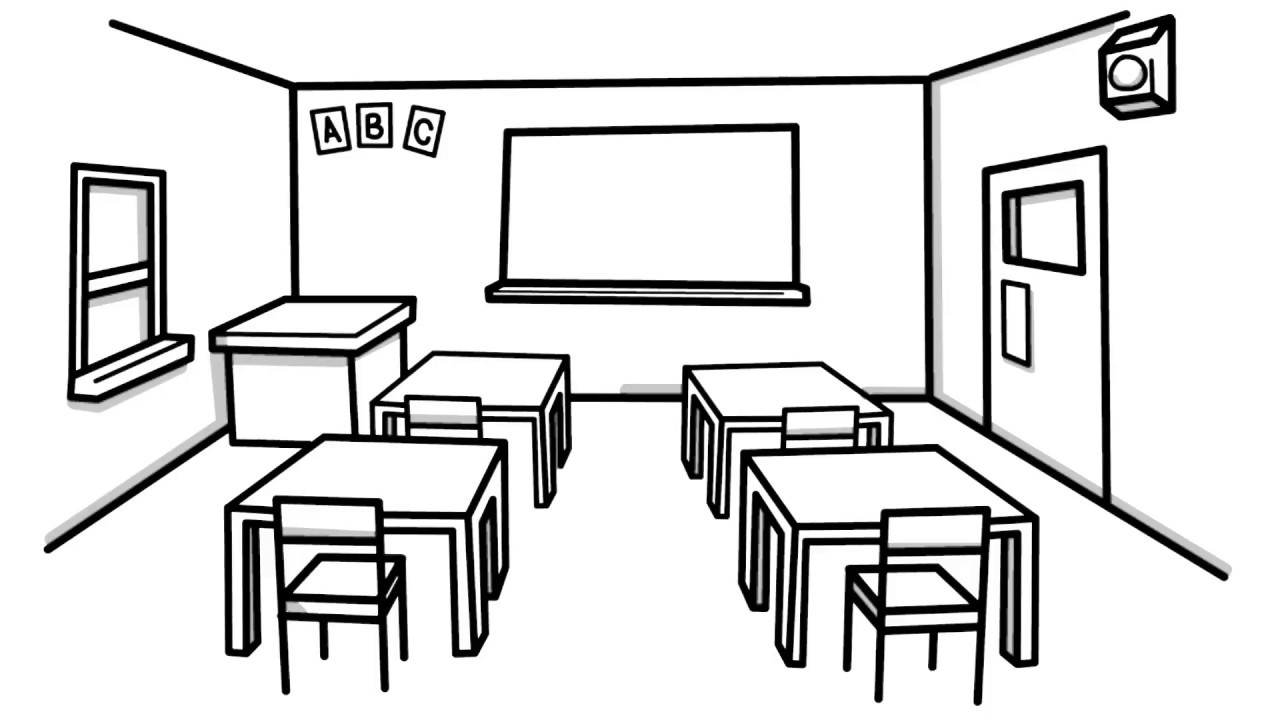
\includegraphics[scale=0.07]{images/room} & 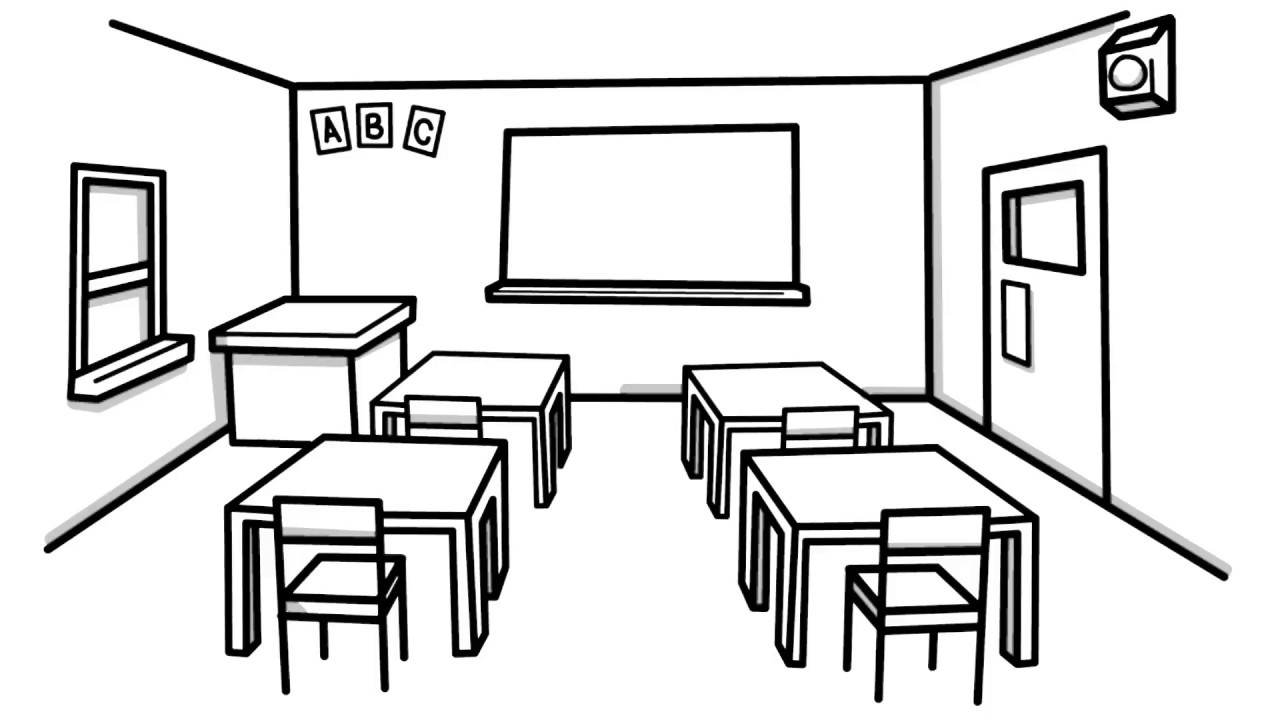
\includegraphics[scale=0.07]{images/room}\\
	\tikz[baseline]{\node[anchor=base] (r1){\only<1-4>{1} \only<5->{\st{1} 2}};} & \tikz[baseline]{\node[anchor=base] (r2){\only<1-4>{2} \only<5->{\st{2} 1}};}\\

	
\end{tabular}



\begin{tabular}{ccc}
	\tikz[baseline]{\node[anchor=base] (g1){};} & \tikz[baseline]{\node[anchor=base] (g2){};} & \tikz[baseline,opacity=0,scale=8,onslide={<2-3>,opacity=1}]{\node[anchor=base] (g3){?};}\\
	
\includegraphics[scale=0.1]{images/south} & 
\includegraphics[scale=0.1]{images/simpson} & 
\includegraphics[scale=0.09]{images/titeuf}\\
	A     & \only<1-4>{B} \only<5->{\st{B} C}         & \only<1-4>{C} \only<5->{\st{C} B}\\
\end{tabular}

\visible<2->{
	\begin{tikzpicture}[overlay]
	\tikzstyle{line} = [<-, line width=0.5mm];
	\path[line]<2> (r1) edge  (g1.south);
	\path[line]<2> (r2) edge  (g2.south);

	\path[line]<3> (r1) edge  (g2.south);
	\path[line]<3> (r2) edge  (g1.south);


%	\path[line,color=blue]<4-> (r1.west) edge  (g1.south);
%	\path[line,color=blue]<4-> (r2) edge  (g3.south);
%
%	\path[line,color=green]<4-> (r1) edge  (g3.south);
%	\path[line,color=gren]<4> (r2.south west) edge  (g1.south);
%
%	\path[line,color=red]<4-> (r1.east) edge  (g2.south);
%	\path[line,color=red]<4-> (r2.east) edge  (g3.south);
%
%	\path[line,color=purple]<4-> (r1) edge  (g3.south);
%	\path[line,color=purple]<4-> (r2) edge  (g2.south);

	\visible<4->{
	\node[draw, minimum width=3cm, minimum height=2cm,line width=0.5mm, color=orange](a) at (-1.75, 4.5) {};
  	\node[draw, minimum width=3cm, minimum height=2cm,line width=0.5mm, color=orange](a) at (1.8, 4.5) {};

	\node[draw, minimum width=3.5cm, minimum height=1.75cm,line width=0.5mm, color=blue](a) at (-3.5, 1.5) {};
	\node[draw, minimum width=3.1cm, minimum height=1.75cm,line width=0.5mm, color=blue](a) at (0.25, 1.5) {};
	\node[draw, minimum width=3.5cm, minimum height=1.75cm,line width=0.5mm, color=blue](a) at (3.9, 1.5) {};
	}
	\end{tikzpicture}
}



\end{frame}

\begin{frame}
	\frametitle{Symmetry in high level}
	\centering
	 g: a symmetry
	\vfill

	\begin{tikzpicture}
		\node[rounded,align=center,minimum height=3cm] (a) {Problem\\ P};
		
		\node [rounded,align=center,minimum height=3cm] (b) at ($(a) + (200pt, 0pt)$){ Problem\\ P'};
		\draw[thick,->] (a) to node [fill=white]{$g$} (b);
		
	\end{tikzpicture}
	\vfill
		\visible<2->{
		\begin{block}{Equi-satisfiability}
			\centering
			$solution \models P \Leftrightarrow g.solution \models P'$
		\end{block}
		
	}

	\vfill
\visible<3->{

\begin{itemize}
	\item Semantic symmetries \hfill \textcolor{UPMCEngagementBlueB}{$\bullet$} \textbf{Syntactic symmetries}
\end{itemize}
	
}
\end{frame}

%% ----------------------------------------------------------------------------
\tikzstyle{every picture}+=[remember picture]
\begin{frame}
\everymath{\displaystyle}

	\frametitle{Syntactic symmetry }
	\normalsize
	A symmetry (permuation) $g$ is a bijective function (on variables) that leaves the formula $\varphi$ invariant
	\vfill
	\visible<2->{
	\scriptsize
	\mbox{$g$ = \bigg(\begin{tabular}{ccccccccc}
		$x_1$ & $x_2$ & $x_3$ & $x_4$ & $x_5$ & $x_6$ & $x_7$ & $x_8$ & $x_9$\\
		$x_2$ & $x_1$ & $x_3$ & $x_5$ & $x_4$ & $x_6$ & $x_8$ & $x_7$ & $x_9$
	\end{tabular}\bigg)}\hfill $\rightarrow$\hfill
	$(x_1 \enskip x_2)(x_4 \enskip x_5)(x_7 \enskip x_8) $\\
	%(\neg x_1 \neg x_2)(\neg x_4 \neg x_5)(\neg x_7 \neg x_8)$\\
}
\visible<3->{
	\vfill
	 \begin{columns}[t]
		\begin{column}[T]{.3\textwidth}
		\tiny
		\begin{itemize}
		\item[] $\omega_{1} = \{x_1  ,  x_2  ,  x_3\} \tikz[baseline]{\node[anchor=base] (a1){};}$
		\item[] $\omega_{2} = \{x_4  ,  x_5  ,  x_6\} \tikz[baseline]{\node[anchor=base] (a2){};}$
		\item[] $\omega_{3} = \{x_7  ,  x_8  ,  x_9\} \tikz[baseline]{\node[anchor=base] (a3){};}$
		\item[] $\omega_{4} = \{\neg x_1  ,  \neg x_4\} \tikz[baseline]{\node[anchor=base] (a4){};}$
		\item[] $\omega_{5} = \{\neg x_1  ,  \neg x_7\} \tikz[baseline]{\node[anchor=base] (a5){};}$
		\item[] $\omega_{6} = \{\neg x_4  ,  \neg x_7\} \tikz[baseline]{\node[anchor=base] (a6){};}$
		\item[] $\omega_{7} = \{\neg x_2  ,  \neg x_5\} \tikz[baseline]{\node[anchor=base] (a7){};}$
		\item[] $\omega_{8} = \{\neg x_2  ,  \neg x_8\} \tikz[baseline]{\node[anchor=base] (a8){};}$
		\item[] $\omega_{9} = \{\neg x_5  ,  \neg x_8\} \tikz[baseline]{\node[anchor=base] (a9){};}$
		\item[] $\omega_{10} = \{\neg x_3  ,  \neg x_6\} \tikz[baseline]{\node[anchor=base] (a10){};}$
		\item[] $\omega_{11} = \{\neg x_3  ,  \neg x_9\} \tikz[baseline]{\node[anchor=base] (a11){};}$
		\item[] $\omega_{12} = \{\neg x_6  ,  \neg x_9\} \tikz[baseline]{\node[anchor=base] (a12){};}$
%		\item[] \qquad \qquad \normalfont{P}
		\end{itemize}
		\end{column}
		\begin{column}[T]{.3\textwidth}
		\tiny
		\begin{itemize}
		\item[] $\tikz[baseline]{\node[anchor=base] (b1){};} \omega_{1} = \{x_2  ,  x_1  ,  x_3\}$
		\item[] $\tikz[baseline]{\node[anchor=base] (b2){};} \omega_{2} = \{x_5  ,  x_4  ,  x_6\} $
		\item[] $\tikz[baseline]{\node[anchor=base] (b3){};} \omega_{3} = \{x_8  ,  x_7  ,  x_9\} $
		\item[] $\tikz[baseline]{\node[anchor=base] (b4){};} \omega_{4} = \{\neg x_2  ,  \neg x_5\} $
		\item[] $\tikz[baseline]{\node[anchor=base] (b5){};} \omega_{5} = \{\neg x_2  ,  \neg x_8\} $
		\item[] $\tikz[baseline]{\node[anchor=base] (b6){};} \omega_{6} = \{\neg x_5  ,  \neg x_8\} $
		\item[] $\tikz[baseline]{\node[anchor=base] (b7){};} \omega_{7} = \{\neg x_1  ,  \neg x_4\} $
		\item[] $\tikz[baseline]{\node[anchor=base] (b8){};} \omega_{8} = \{\neg x_1  ,  \neg x_7\} $
		\item[] $\tikz[baseline]{\node[anchor=base] (b9){};} \omega_{9} = \{\neg x_4  ,  \neg x_7\} $
		\item[] $\tikz[baseline]{\node[anchor=base] (b10){};} \omega_{10} = \{\neg x_3  ,  \neg x_6\} $
		\item[] $\tikz[baseline]{\node[anchor=base] (b11){};} \omega_{11} = \{\neg x_3  ,  \neg x_9\} $
		\item[] $\tikz[baseline]{\node[anchor=base] (b12){};} \omega_{12} = \{\neg x_6  ,  \neg x_9\} $
%				\item[] \qquad \normalfont{g.P = P' = P}
	\end{itemize}
	\end{column}
\end{columns}

\begin{tikzpicture}[overlay]
\tikzstyle{line} = [<->];
\path[line] (a1) edge  (b1);
\path[line] (a2) edge  (b2);
\path[line] (a3) edge  (b3);
\path[line] (a4) edge  (b7);
\path[line] (a5) edge  (b8);
\path[line] (a6) edge  (b9);
\path[line] (a7) edge  (b4);
\path[line] (a8) edge  (b5);
\path[line] (a9) edge  (b6);
\path[line] (a10) edge  (b10);
\path[line] (a11) edge  (b11);
\path[line] (a12) edge  (b12);

\end{tikzpicture}
}

\visible<3>{
\begin{tikzpicture}[overlay]
\node[](p) at (15pt, 75pt) {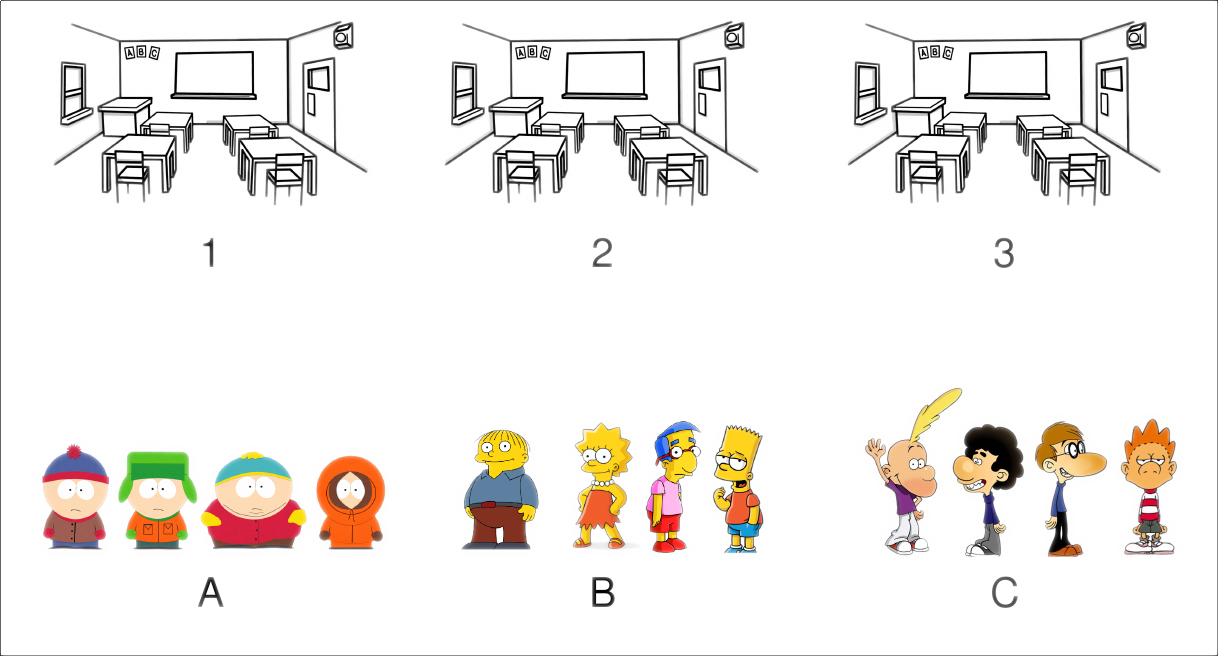
\includegraphics[width=.2\textwidth]{images/plan2}};
\node[](p) at (300pt, 75pt) {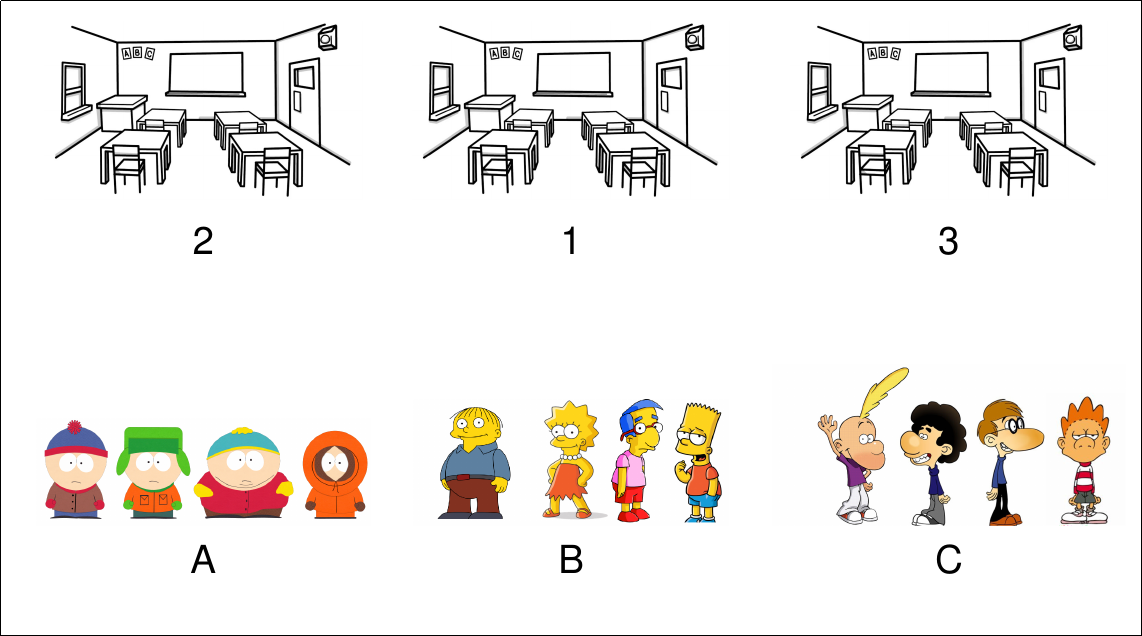
\includegraphics[width=.2\textwidth]{images/planinv}};
\node[](p) at (80pt, -10pt) {P};
\node[](p) at (232pt, -10pt) {g.P = P' = P};

\end{tikzpicture}
}
\end{frame}


\begin{frame}
	\frametitle{Computing symmetries of a SAT problem}
	% \setlength{\tabcolsep}{35pt}

	\newcolumntype{C}{ >{\centering\arraybackslash} m{5cm} }
	\newcolumntype{D}{ >{\centering\arraybackslash} m{1cm} }
	\begin{tabular}{CC}
		$CNF\ formula$ &{\scriptsize
			\begin{tabular}{c}
				$(x_1 \lor x_2 \lor x_3) \land
				(x_4 \lor x_5 \lor x_6) \land
				(x_7 \lor x_8 \lor x_9) $\\
				$\land (\neg x_1 \lor \neg x_4) \land
				(\neg x_1 \lor \neg x_7) \land
				(\neg x_4 \lor \neg x_7)$\\
				$\land (\neg x_2 \lor \neg x_5) \land
				(\neg x_2 \lor \neg x_8) \land
				(\neg x_5 \lor \neg x_8)$ \\
				$\land (\neg x_3 \lor \neg x_6) \land
				(\neg x_3 \lor \neg x_9) \land
				(\neg x_6 \lor \neg x_9)$\\
		\end{tabular}}\\
		\only<2> {
			$\Downarrow$ & $\Downarrow$  \\

			colored graph &
			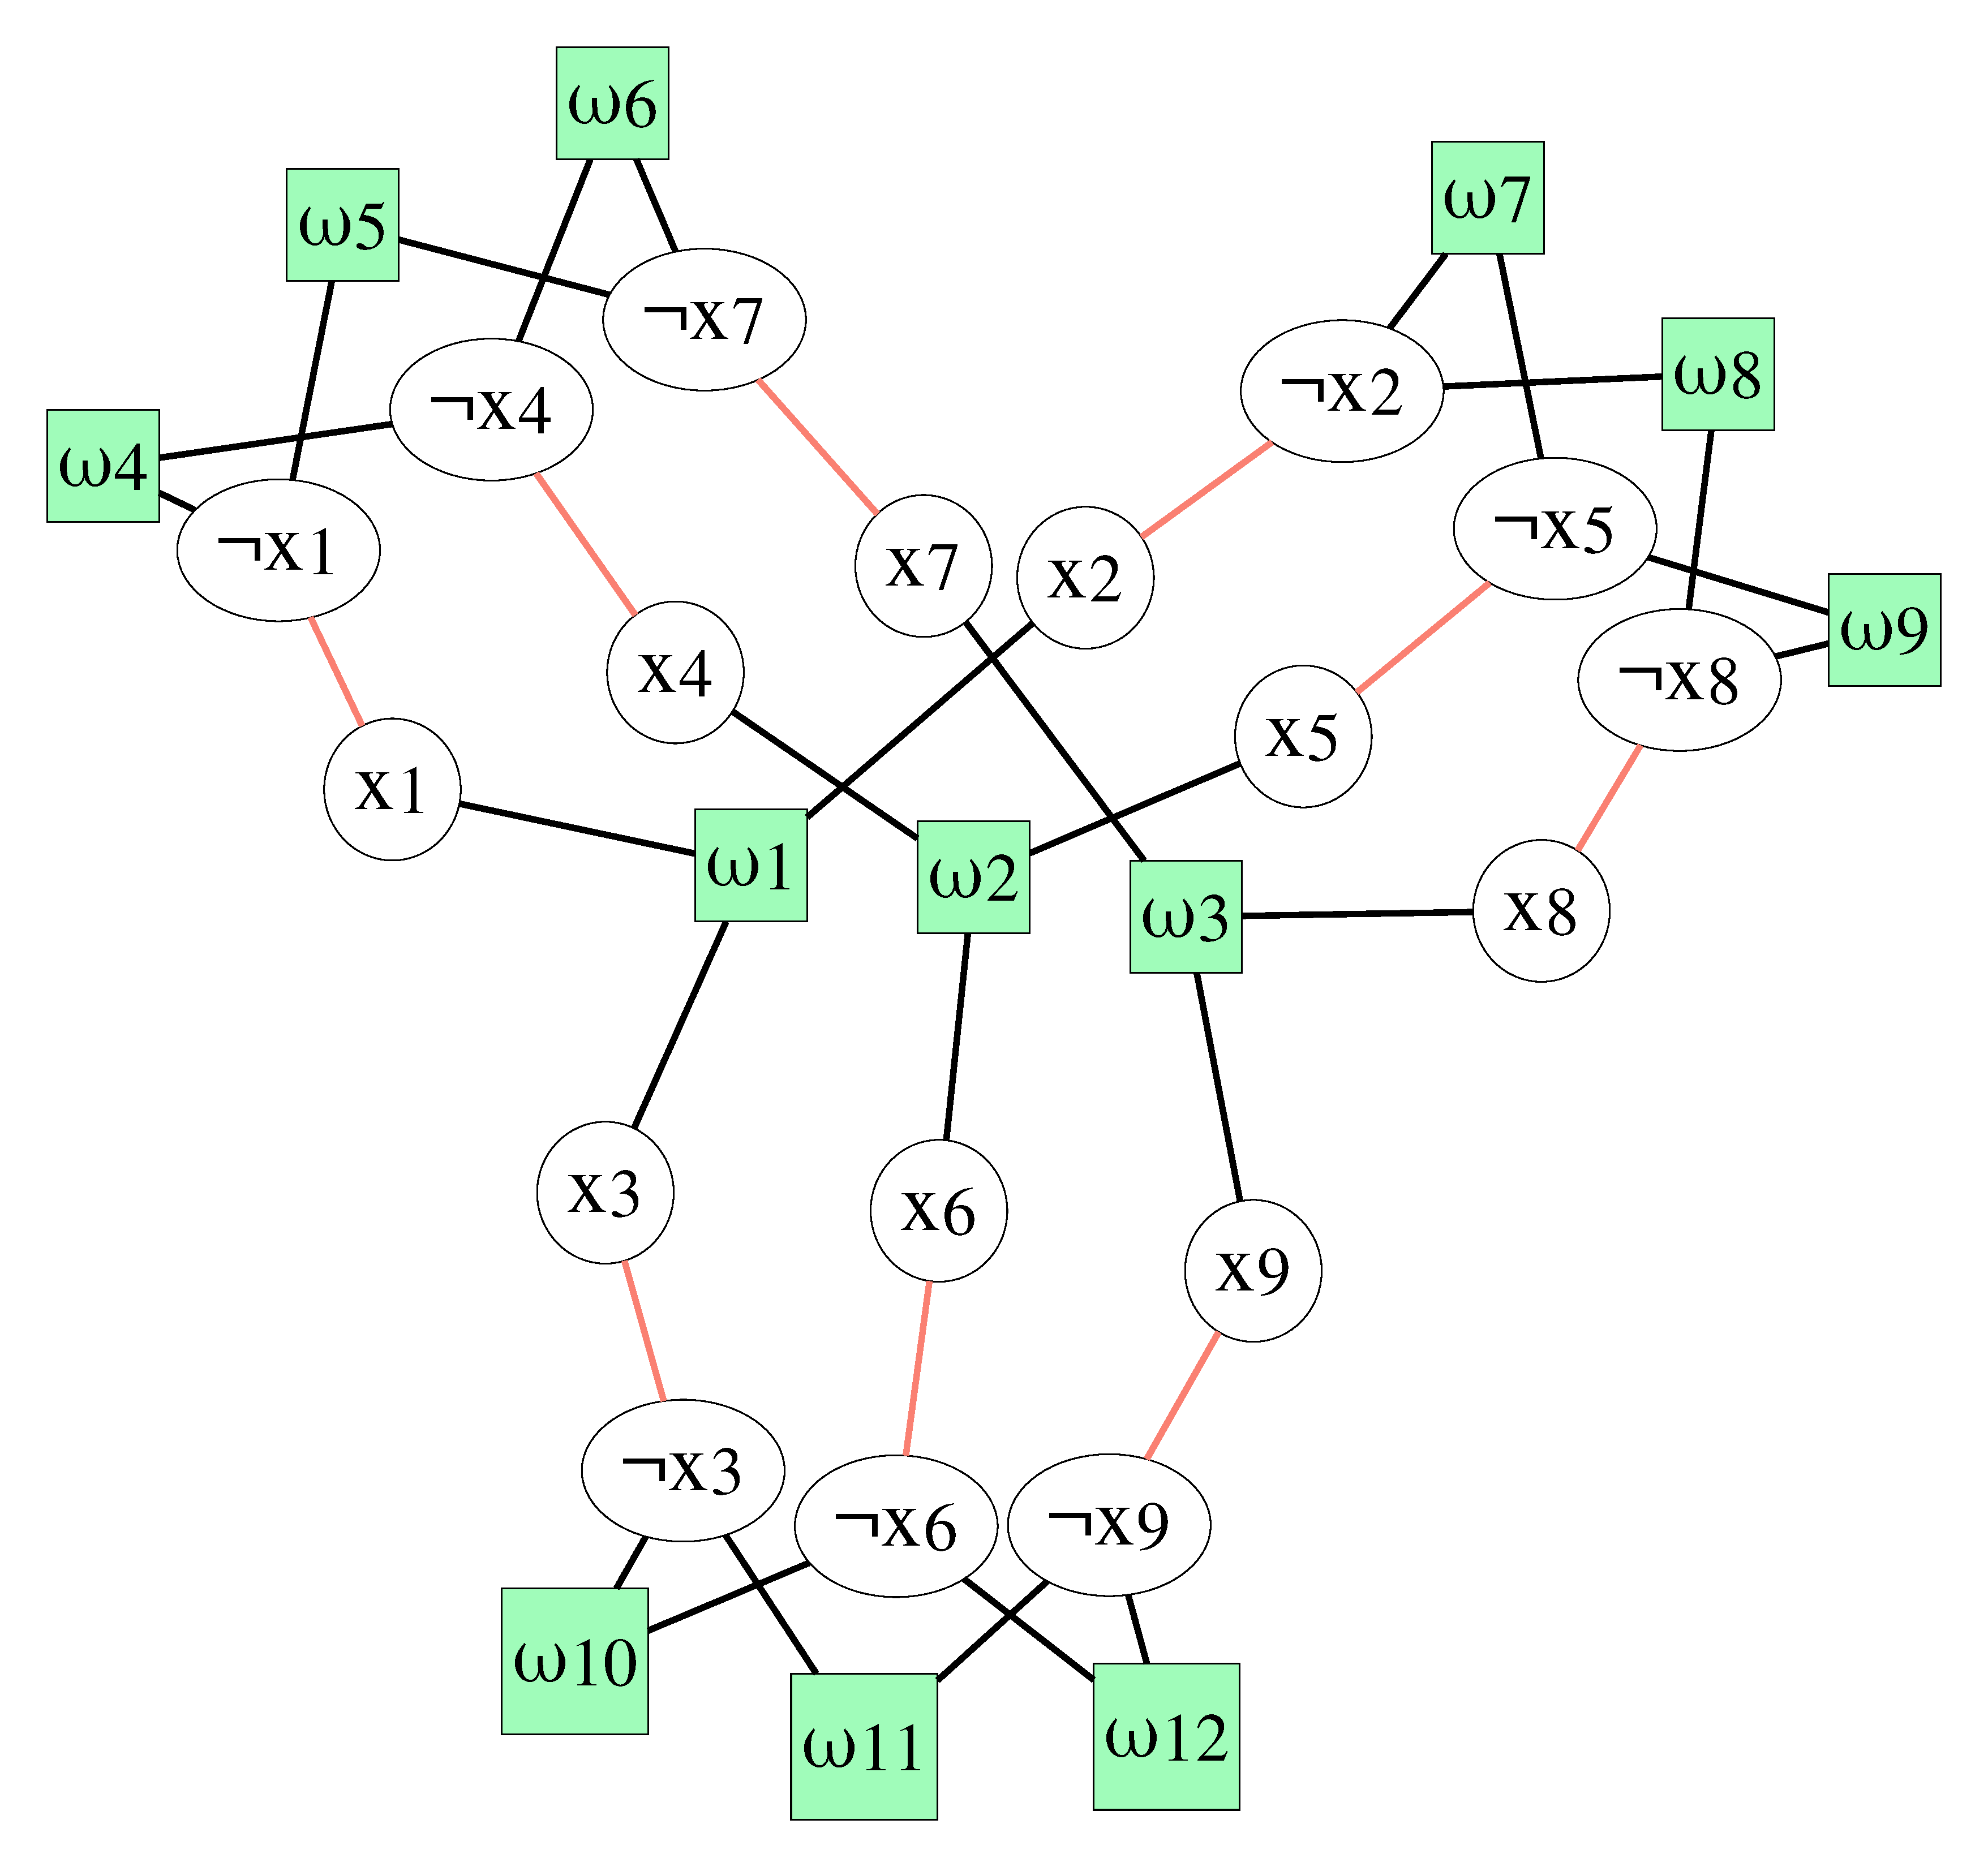
\includegraphics[scale=0.1]{images/graph}\\ \\
		}

		\visible<3-> {

			$\Downarrow$ & $\Downarrow$  \\

			colored graph &
			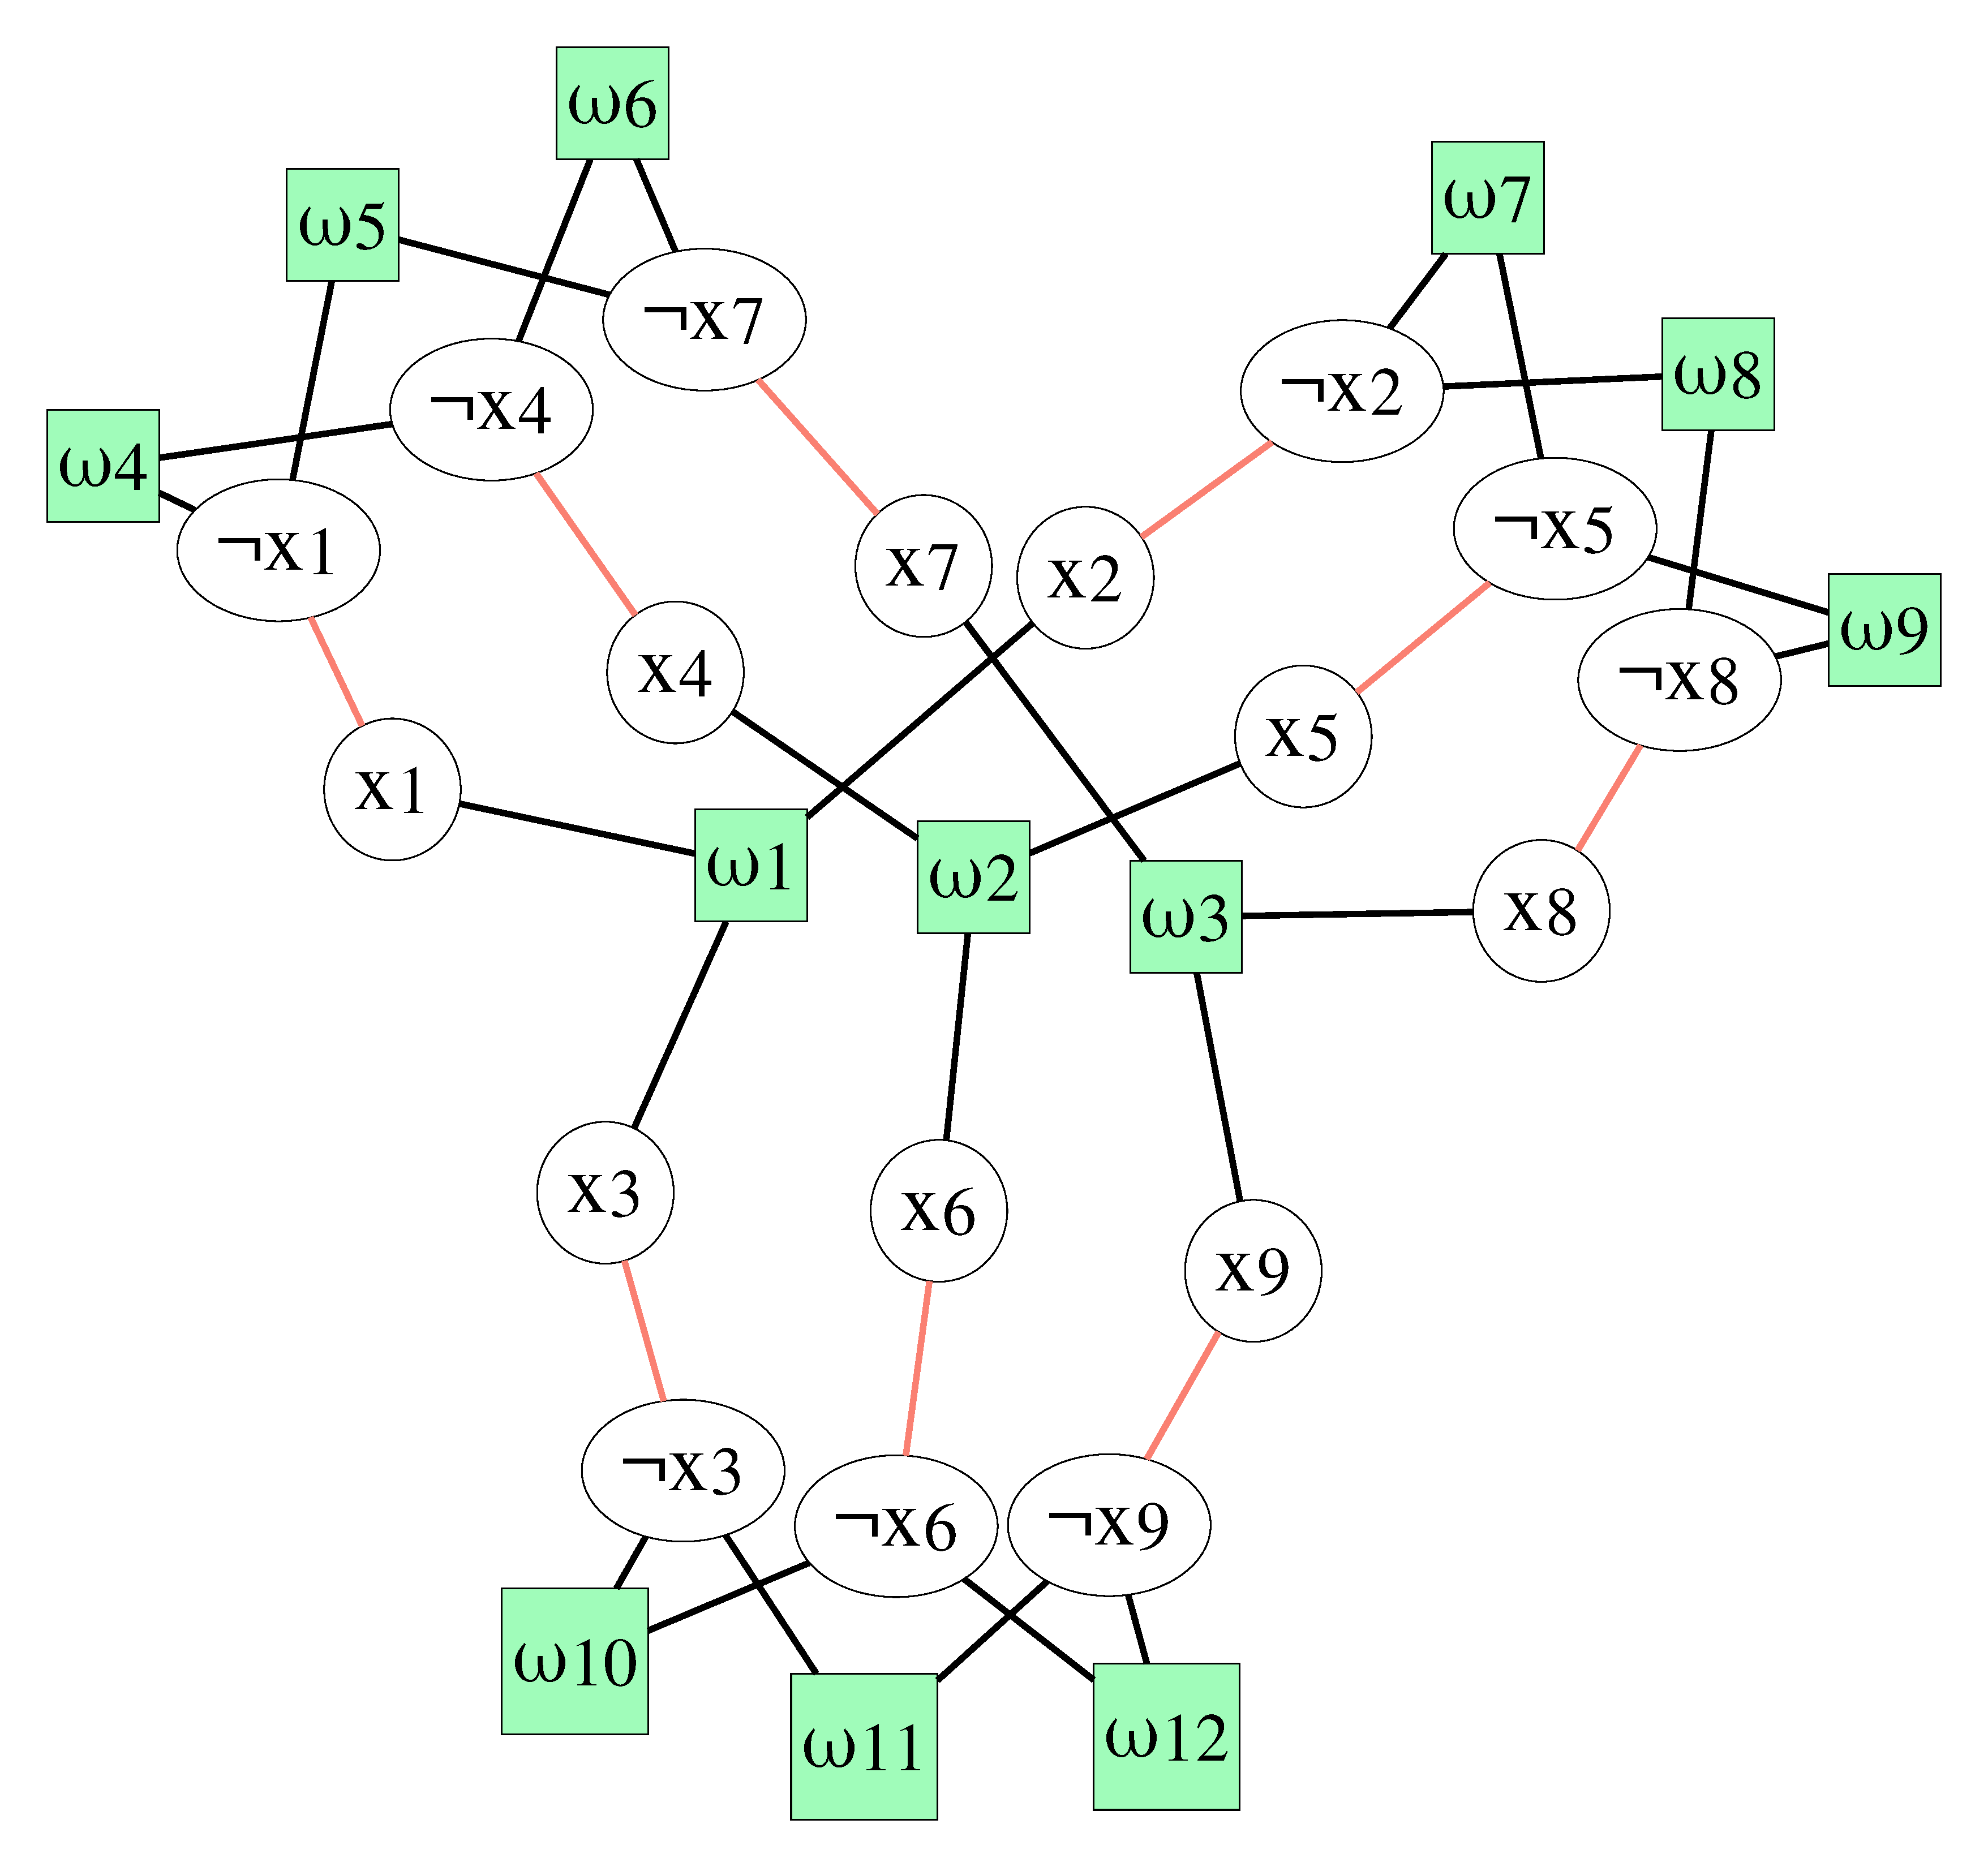
\includegraphics[scale=0.05]{images/graph}\\ \\
		}


		\visible<3-> {
			$\|$ & $\|$  \\
			graph automorphism &
			\small{(\texttt{bliss},	\texttt{saucy}, $\ldots$)
			}
			\\
		}


		\visible<4-> {
			$\Downarrow$ & $\Downarrow$  \\

			set of symmetries &
			\scriptsize
			\begin{tabular}{c}
				$g_1 = (x_2 \enspace x_3)(x_5 \enspace x_6)(x_8 \enspace x_9)$\\
				$g_2 = (x_4 \enspace x_7)(x_5 \enspace x_8)(x_6 \enspace x_9)$\\
				$g_3 = (x_1 \enspace x_2)(x_4 \enspace x_5)(x_7 \enspace x_8)$\\
				$g_4 = (x_1 \enspace x_4)(x_2 \enspace x_5)(x_3 \enspace x_6)$
			\end{tabular}
		}
	\end{tabular}
\vfill
	\visible<4-> { \centering \small The set of symmetries of a formula is a group noted $<\mathit{G,\circ}>$}
\end{frame}

\begin{frame}
	\centering
	\textcolor{UPMCEngagementBlueB}{\Large Exploitation of symmetries:}\\
\vspace{2em}
	\textcolor{UPMCEngagementBlueB}{\Large Static symmetry breaking}
\end{frame}




\begin{frame}
\frametitle{Orbit}

\begin{center}
	Orbit of an assignment $\alpha$ for a group $G$: $$G.\alpha = \{ g.\alpha \mid g \in G \}$$
\end{center}

\vfill
\visible<2->{
Example:
\begin{columns}[t]
	\begin{column}[T]{.3\textwidth}
		\begin{tabular}{cl}
			\begin{tikzpicture}
			\node[point] at (0,0){};
			\end{tikzpicture} & full assignment \\
			\visible<4->{
				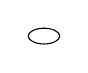
\begin{tikzpicture}
				\node[class2, scale=0.2] at (0,0){};
				\end{tikzpicture} & orbit  \\
			}
		\visible<5>{
			
\begin{tikzpicture}
		\node[point+] at (0,0){};
		\end{tikzpicture} & representative   \\
		}
		\end{tabular}
	\end{column}
	\begin{column}[T]{0.6\textwidth}
		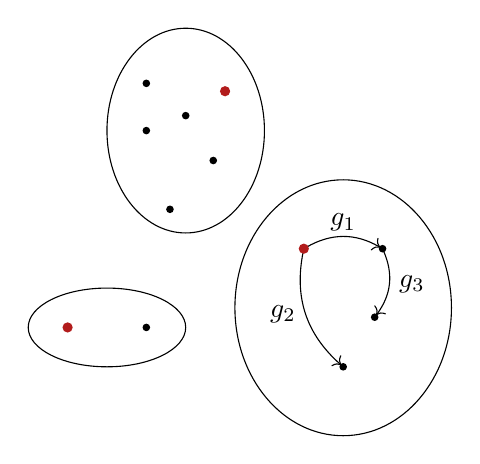
\begin{tikzpicture}

		\tikzstyle{class2}=[ellipse, draw, minimum width=2cm, minimum height=1cm]
		\tikzstyle{class1}=[ellipse, draw, minimum width=1cm, minimum height=1cm]

		\visible<2-> {
			\begin{scope}
			\node[point] (p1) at (0, 0){};
			\node[point] (p2) at (1, 0){};
			\node[point] (p3) at (-2, -1){};
			\node[point] (p4) at (-3, -1){};
			\node[point] (p5) at (-1.7, 0.5){};
			\node[point] (p6) at (-2, 1.5){};

			\node[point] (p6) at (-1.5, 1.69){};

			\node[point] (p6) at (-1.15, 1.12){};

			\node[point] (p6) at (-2, 2.1){};


			\node[point] (p66) at (0.5, -1.5){};

			\node[point] (p77) at (0.9, -0.87){};


			\node[point] (p8) at (-1, 2){};
\visible<3->{
			\draw[,->] (p1) to [bend left=30] node [midway,  align=center,yshift=.5em] {$g_1$}  (p2);
			%\draw[,->] (p2) to [bend left=30] node [midway,  align=center,yshift=-.6em] {$g^{-1}_1$}  (p1);
			\draw[,->] (p1)  to [bend right=30] node [midway, align=center,left] {$g_2$} (p66);
			\draw[,->] (p2)  to [bend left=30] node [midway, align=center,right] {$g_3$} (p77);
		}
\visible<5>{
			\node[point+] (p1) at (0, 0){};
			\node[point+] (p4) at (-3, -1){};
			\node[point+] (p8) at (-1, 2){};
}
			\end{scope}
		}

		\visible<4-> {
			\begin{scope}

			\node[class2] (c2) at (-2.5, -1){};

			\node[ellipse, draw, minimum width=2cm, minimum height=2.6cm] (c3) at (-1.5, 1.5) {};
			\node[ellipse, draw, minimum width=2.75cm, minimum height=3.25cm] (c4) at (0.5, -0.75) {};

			\end{scope}
		}

		\end{tikzpicture}
	\end{column}
\end{columns}
}
\vfill

\visible<4->{
	Equivalence relation with respect to SAT:
	\begin{itemize}
		\item Either $G.\alpha$ contains no solution
		\item Or all elements of $G.\alpha$ are solutions
	\end{itemize}
}
%\textbf{Legend:}\\
%\begin{tabular}{cl}
%\begin{tikzpicture}
%\node[point] at (0,0){};
%\end{tikzpicture} & full assignment \\
%\visible<2->{
%	\begin{tikzpicture}
%	\node[class2, scale=0.2] at (0,0){};
%	\end{tikzpicture} & orbits } \\
%\visible<3->{
%	\begin{tikzpicture}
%	\node[point+] at (0,0){};
%	\end{tikzpicture} & representant of the orbit\\
%}
%\end{tabular}


\end{frame}


\begin{frame}
	\frametitle{Comparing assignments: Assessments}
	
	Define an ordering relation to compare assignments ($\prec$)
	\begin{itemize}
		\item Total ordering on variables
		\item Minimum value: $\false < \true$ or $\true < \false$
	\end{itemize}

\vfill
\visible<2->{
	\begin{center}
			\textbf{Allow only minimal value (lex-leader)}\\
	\end{center}
}

	\vfill
	\visible<3>{
	Forbid other assignments in each orbit\\
	$\enspace \rightarrow$ Add all symmetry breaking predicates (SBP) statically
	}


\end{frame}

\begin{frame}
		\frametitle{Comparing assignments: Example}

Ordering relation: $x_1 \leq x_2 \leq x_3  \leq x_4 \leq x_5 \leq x_6 \leq x_7 \leq x_8 ;  \false < \true$
%		\begin{itemize}
%			\item[]	$x_1 \leq x_2 \leq x_3  \leq x_4 \leq x_5 \leq x_6 \leq x_7 \leq x_8 ;  \false < \true$
%		\end{itemize}
	
\vfill		
Symmetry:	$g = (x_1 \enskip x_2)(x_4 \enskip x_5)(x_7 \enskip x_8) $\\
%		\begin{itemize}
%
%			\item[] 	$g = (x_1 \enskip x_2)(x_4 \enskip x_5)(x_7 \enskip x_8) $\\
%		\end{itemize}
%		\vfill

\vfill		
Assignments:		
		\begin{center}
			\begin{tabular}{cccccccccc}
				
				& $x_1$ & $x_2$ & $x_3$ & $x_4$ & $x_5$ & $x_6$ & $x_7$& $x_8$ \\
				\toprule
				$\alpha$ &\true & \false  & \false & \false & \false & \false& \false& \false \\
				&&&&&&&&\\
				\visible<2->{$g.\alpha$ &\false & \true  & \false & \false & \false & \false& \false& \false} \\
				
			\end{tabular}
		\end{center}
\vfill
\visible<3->{
Comparing:
}		

		\centering \visible<3->{ $g.\alpha \prec \alpha$} \visible<4->{$\Rightarrow$  SBP: $\omega = \{ \neg x_1, x_2\}$}
\end{frame}
%% ----------------------------------------------------------------------------
\begin{frame}
	\frametitle{Using symmetries to prune the search space}
\only<1>{$g = (x_1 \enskip x_2)(x_4 \enskip x_5)(x_7 \enskip x_8) $ \hfill $\omega = \{ \neg x_1, x_2\}$\\}
\only<2>{$g = \textcolor{blue}{(x_1 \enskip x_2)}(x_4 \enskip x_5)(x_7 \enskip x_8) $\hfill $\omega = \{ \neg x_1, x_2\}$\\}
	\centering
	\begin{tikzpicture}[scale=1, every node/.style={scale=1}]

	\newcommand{\x}{2.07}
	\newcommand{\y}{-1.5}
	\tikzstyle{highlight} = [line width=0.3mm, color=blue]
	\tikzstyle{decision}=[circle,draw,thick,fill=blue!30,font=\scriptsize]
%	\tikzstyle{unsat}=[draw,thick, fill=red]
	\tikzstyle{unsat}=[scale=2, fill=white]
	\tikzstyle{link}=[->,>=latex,rounded corners=5pt,thick]
	\tikzstyle{transparent} = [nearly transparent]
	\tikzstyle{mid}=[midway,fill=white,nearly transparent,opacity=1, text opacity=1,font=\scriptsize]
	\tikzstyle{trmid}=[midway,fill=white,nearly transparent,opacity=1, text opacity=0.3,font=\scriptsize]

	% layer 1
	\node[decision](t) at (0,0) {$x_1$};

	% layer 2
	\node[decision](l) at (-\x,\y) {$x_2$};
	\node[decision](r) at (\x,\y) {$x_2$};

	\visible<2>{\node[highlight, scale=2](equiv) at (0,\y) {$\leftrightarrow$};}

	% layer 3
	\node[decision](ll) at (-\x-\x*0.5,2*\y) {$x_4$};
	\node[decision](lr) at (-\x+\x*0.5,2*\y) {$x_4$};
	\node[decision,onslide={<2>, transparent}](rl) at (\x-\x*0.5,2*\y) {$x_4$};
	\node[decision](rr) at (\x+\x*0.5,2*\y) {$x_4$};

	% layer 4
	\node[decision](lll) at (-\x-\x*0.5-\x*0.25,3*\y) {$x_5$};
	\node[decision](llr) at (-\x-\x*0.5+\x*0.25,3*\y) {$x_5$};
	\node[decision](lrl) at (-\x+\x*0.5-\x*0.25,3*\y) {$x_5$};
	\node[decision](lrr) at (-\x+\x*0.5+\x*0.25,3*\y) {$x_5$};
	\node[decision,onslide={<2>, transparent}](rll) at (\x-\x*0.5-\x*0.25,3*\y) {$x_5$};
	\node[decision,onslide={<2>, transparent}](rlr) at (\x-\x*0.5+\x*0.25,3*\y) {$x_5$};
	\node[decision](rrl) at (\x+\x*0.5-\x*0.25,3*\y) {$x_5$};
	\node[decision](rrr) at (\x+\x*0.5+\x*0.25,3*\y) {$x_5$};

	% layer 5
	\node[unsat](llll) at (-\x-\x*0.5-\x*0.25-\x*0.125,4*\y) {\pgfuseplotmark{triangle}};
	\node[unsat](lllr) at (-\x-\x*0.5-\x*0.25+\x*0.125,4*\y) {\pgfuseplotmark{triangle}};
	\node[unsat](llrl) at (-\x-\x*0.5+\x*0.25-\x*0.125,4*\y) {\pgfuseplotmark{triangle}};
	\node[unsat](llrr) at (-\x-\x*0.5+\x*0.25+\x*0.125,4*\y) {\pgfuseplotmark{triangle}};
	\node[unsat](lrll) at (-\x+\x*0.5-\x*0.25-\x*0.125,4*\y) {\pgfuseplotmark{triangle}};
	\node[unsat](lrlr) at (-\x+\x*0.5-\x*0.25+\x*0.125,4*\y) {\pgfuseplotmark{triangle}};
	\node[unsat](lrrl) at (-\x+\x*0.5+\x*0.25-\x*0.125,4*\y) {\pgfuseplotmark{triangle}};
	\node[unsat](lrrr) at (-\x+\x*0.5+\x*0.25+\x*0.125,4*\y) {\pgfuseplotmark{triangle}};
	\node[unsat,onslide={<2>, transparent}](rlll) at (\x-\x*0.5-\x*0.25-\x*0.125,4*\y) {\pgfuseplotmark{triangle}};
	\node[unsat,onslide={<2>, transparent}](rllr) at (\x-\x*0.5-\x*0.25+\x*0.125,4*\y) {\pgfuseplotmark{triangle}};
	\node[unsat,onslide={<2>, transparent}](rlrl) at (\x-\x*0.5+\x*0.25-\x*0.125,4*\y) {\pgfuseplotmark{triangle}};
	\node[unsat,onslide={<2>, transparent}](rlrr) at (\x-\x*0.5+\x*0.25+\x*0.125,4*\y) {\pgfuseplotmark{triangle}};
	\node[unsat](rrll) at (\x+\x*0.5-\x*0.25-\x*0.125,4*\y) {\pgfuseplotmark{triangle}};
	\node[unsat](rrlr) at (\x+\x*0.5-\x*0.25+\x*0.125,4*\y) {\pgfuseplotmark{triangle}};
	\node[unsat](rrrl) at (\x+\x*0.5+\x*0.25-\x*0.125,4*\y) {\pgfuseplotmark{triangle}};
	\node[unsat](rrrr) at (\x+\x*0.5+\x*0.25+\x*0.125,4*\y) {\pgfuseplotmark{triangle}};


	\draw[link, onslide={<2>, highlight}] (t) ->  node [mid] {$0$} (l);
	\draw[link, onslide={<2>, highlight}] (t) -> node [mid] {$1$} (r);

	\draw[link] (l) ->  node [mid] {$0$} (ll);
	\draw[link,onslide={<2>, highlight}] (l) -> node [mid] {$1$} (lr);
	\draw[link,onslide={<2>, highlight}] (r) ->  node [mid] {$0$} (rl);
	\draw[link] (r) -> node [mid] {$1$} (rr);

	\draw[link] (ll) -> node [mid] {$0$} (lll);
	\draw[link] (ll) -> node [mid] {$1$} (llr);
	\draw[link] (lr) -> node [mid] {$0$} (lrl);
	\draw[link] (lr) -> node [mid] {$1$} (lrr);

	\draw[link,onslide={<2>, transparent}] (rl) -> node [mid,onslide={<2>, trmid}] {$0$} (rll);
	\draw[link,onslide={<2>, transparent}] (rl) -> node [mid,onslide={<2>, trmid}] {$1$} (rlr);
	\draw[link] (rr) -> node [mid] {$0$} (rrl);
	\draw[link] (rr) -> node [mid] {$1$} (rrr);


	\draw[link] (lll) -> node [mid] {$0$} (llll);
	\draw[link] (lll) -> node [mid] {$1$} (lllr);
	\draw[link] (llr) -> node [mid] {$0$} (llrl);
	\draw[link] (llr) -> node [mid] {$1$} (llrr);
	\draw[link] (lrl) -> node [mid] {$0$} (lrll);
	\draw[link] (lrl) -> node [mid] {$1$} (lrlr);
	\draw[link] (lrr) -> node [mid] {$0$} (lrrl);
	\draw[link] (lrr) -> node [mid] {$1$} (lrrr);

	\draw[link,onslide={<2>, transparent}] (rll) -> node [mid,onslide={<2>, trmid}] {$0$} (rlll);
	\draw[link,onslide={<2>, transparent}] (rll) -> node [mid,onslide={<2>, trmid}] {$1$} (rllr);
	\draw[link,onslide={<2>, transparent}] (rlr) -> node [mid,onslide={<2>, trmid}] {$0$} (rlrl);
	\draw[link,onslide={<2>, transparent}] (rlr) -> node [mid,onslide={<2>, trmid}] {$1$} (rlrr);
	\draw[link] (rrl) -> node [mid] {$0$} (rrll);
	\draw[link] (rrl) -> node [mid] {$1$} (rrlr);
	\draw[link] (rrr) -> node [mid] {$0$} (rrrl);
	\draw[link] (rrr) -> node [mid] {$1$} (rrrr);
	\end{tikzpicture}
	\vfill
%\visible<2> {Add symmetry breaking predicates to prune the  search space.}
\end{frame}


%\begin{frame}
% \frametitle{Representative assignment}
%
%
%\begin{center}
%
%		\begin{tikzpicture}
%		
%		\tikzstyle{class2}=[ellipse, draw, minimum width=2cm, minimum height=1cm]
%		\tikzstyle{class1}=[ellipse, draw, minimum width=1cm, minimum height=1cm]
%		
%
%			\begin{scope}
%			
%
%			%	\node[](a3) at (0, 0.25) {$\alpha_3$};
%			
%			\node[point] (p2) at (1, 0){};
%			%	\node[](a5) at (1, 0.25) {$\alpha_5$};
%			
%			\node[point] (p3) at (-2, -1){};
%			%	\node[](a6) at (-2, -0.75) {$\alpha_6$};
%			
%
%			%	\node[](a4) at (-3, -0.75) {$\alpha_4$};
%			
%			\node[point] (p5) at (-1.7, 0.5){};
%			%	\node[](a1) at (-1.7, 0.75) {$\alpha_1$};
%			
%			\node[point] (p6) at (-2, 1.5){};
%			
%			\node[point] (p6) at (-1.5, 1.69){};
%			
%			\node[point] (p6) at (-1.15, 1.12){};
%			
%			\node[point] (p6) at (-2, 2.1){};
%			%	\node[](a2) at (-2, 1.75) {$\alpha_2$};
%			
%			\node[point] (p7) at (0.5, -1.5){};
%			
%			\node[point] (p7) at (0.9, -0.87){};
%			%	\node[](a7) at (0.5, -1.25) {$\alpha_7$};
%			
%						\node[point+] (p1) at (0, 0){};
%						\node[point+] (p4) at (-3, -1){};
%			\node[point+] (p8) at (-1, 2){};
%			%	\node[](a8) at (-1, 2.25) {$\alpha_8$};
%			
%			\end{scope}
%		
%		
%			\begin{scope}
%			
%			%\node[class2] (c1) at (0.5,0){};
%			\node[class2] (c2) at (-2.5, -1){};
%			
%			\node[ellipse, draw, minimum width=2cm, minimum height=2.6cm] (c3) at (-1.5, 1.5) {};
%			\node[ellipse, draw, minimum width=2cm, minimum height=2.75cm] (c4) at (0.5, -0.75) {};
%
%			\end{scope}
%		
%
%		\end{tikzpicture}
%\end{center}
%
%		\begin{tabular}{cl}
%	\begin{tikzpicture}
%	\node[point] at (0,0){};
%	\end{tikzpicture} & full assignment \\
%	\begin{tikzpicture}
%	\node[class2, scale=0.2] at (0,0){};
%	\end{tikzpicture} & orbit  \\
%	\begin{tikzpicture}
%	\node[point+] at (0,0){};
%	\end{tikzpicture} & representative assignment  \\
%\end{tabular}
%\end{frame}
%




%% ----------------------------------------------------------------------------
\begin{frame}
\frametitle{State-of-the-art static symmetry breaking}


State-of-the-art:
\begin{itemize}
	\item Shatter \cite{aloul06} \hfill \textcolor{UPMCEngagementBlueB}{$\bullet$}  BreakID \cite{devriendt2016improved}
\end{itemize}
\vfill
\begin{center}
\begin{tikzpicture}
	\tikzstyle{box} = [draw, minimum width=1.5cm]

	\node[box,minimum height=1.2cm] (cnf) {CNF};
	\node[box] (sym) at (-3, -1) { Symmetries};
	\node[box,minimum height=1.2cm,onslide={<4>, starburst,draw=red,line width=0.5mm}] (sbp) at (0, -2) { SBPs};

	
	\node[box, minimum height=3.5cm, minimum width=2cm, line width=0.5mm, opacity=0,onslide={<2->, opacity=1}] at (0, -1) (full) {$\land$};
	\node[box,minimum height=1.2cm, opacity=0, onslide={<2->,opacity=1}] (solver) at (3, -1) { SAT solver};

	\draw[->, thick, bend left = 30] (cnf) to [bend right=30] node [midway, left, fill=white] {compute symmetries} (sym);
	\draw[->, thick, bend left = 30] (sym) to [bend right=30] node [midway, left, fill=white] {generates SBPs} (sbp);

	\draw[->, thick, opacity=0, onslide={<2->,opacity=1}] (full) to [] (solver);
\end{tikzpicture}
\end{center}
\vfill



\vfill
\visible<3->{
\textcolor{green}{Works well on many symmetrical problems}\\
}
\vfill
\visible<4>{
 \textcolor{red}{The solver can "explode" instead of being helped}
\begin{itemize}
	\item \color{red}generate not needed clause
	\item \color{red}flooding the solver
\end{itemize}
}
\end{frame}



\begin{frame}
\centering
\textcolor{UPMCEngagementBlueB}{\Large First contribution: }\\
\vspace{2em}
\textcolor{UPMCEngagementBlueB}{\Large CDCL[sym] Introducing Effective Symmetry Breaking in SAT Solving }\\
\vspace{2em}
\textcolor{UPMCEngagementBlueB}{\Large  TACAS'18~\cite{metin2018cdclsym}}
\end{frame}



%% ----------------------------------------------------------------------------
%\begin{frame}
%\frametitle{Our contribution CDCL[Sym]}
%
%Tackling the explosion problem in the static symmetry breaking approaches.
%
%
%Compute and inject ESBP \textcolor{hgreen}{opportunistically} during the solving\\
%
%\end{frame}
%


%% ----------------------------------------------------------------------------

\begin{frame}
	\frametitle{General idea}
	
	
	\begin{center}
		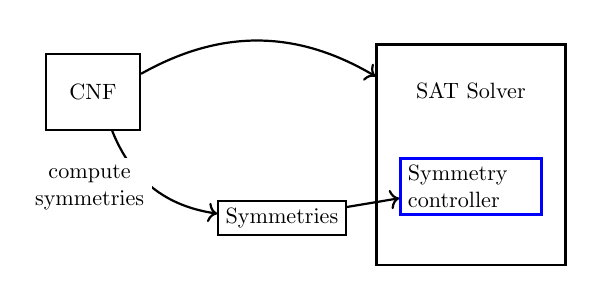
\begin{tikzpicture}[scale=0.8,every node/.style={scale=0.8}]
		\tikzstyle{box} = [draw, minimum width=1.5cm]
		
		\node[box,thick,minimum height=1.2cm] (cnf) at (-5, 0) {CNF};
		\node[box,thick] (sym) at (-2, -2) { Symmetries};
		
		
		\node[box,thick,minimum width=3cm,minimum height=3.5cm,label={[yshift=-1cm]SAT Solver}] (solver) at (1, -1) { };
		\node[box,text width=2cm,thick,line width=0.4mm,draw=blue] (symcomp) at (1, -1.5) {Symmetry controller};
		\draw[->, thick, bend left = 30] (cnf) to [bend right=30] node [midway, left, fill=white, align=center] {compute\\symmetries} (sym);
		
		\draw[->, thick,bend left = 30] (cnf) to [] (solver);
		\draw[->, thick] (sym) to [] (symcomp);
		\end{tikzpicture}
	\end{center}
	\vfill
	
	Symmetry controller:
	\begin{itemize}
		\item \textcolor{green}{Generates SBP on-the-fly}
		\item \textcolor{green}{Only when needed}
		\item \textcolor{red}{Intrusive on solver}
	\end{itemize}

\end{frame}

\begin{frame}
\frametitle{CDCL[Sym]}

Compute and inject SBP \textcolor{blue}{opportunistically}, during the solving

\vspace{1em}

\centering
\begin{tikzpicture}[scale=0.9,every node/.style={scale=0.5,fill=white, font=\sffamily}, align=center]
% Specification of nodes (position, etc.)
\tikzset{%
	>={Latex[width=2mm,length=2mm]},
	% Specifications for style of nodes:
	base/.style = {rectangle, rounded corners, draw=black,
		minimum width=2cm, minimum height=1cm,
		text centered, font=\sffamily},
	question/.style = {base, diamond, fill=blue!15},
	question/.style = {base, diamond, fill=blue!15},
	unsat/.style = {base, fill=red!30,minimum width=3cm},
	sat/.style = {base, fill=green!30,minimum width=3cm},
	process/.style = {base, minimum width=2.5cm, fill=orange!25,
		font=\ttfamily},
	processcurr/.style = {process, thick, line width=0.7mm, draw=purple!80 },
	questioncurr/.style = {question,line width=0.7mm, draw=purple!80},
	line/.style = {->, thick },
	linecurr/.style = {line, line width=0.7mm, draw=purple!80},
}

\node (isfin) [question,onslide={<2->,fill=black!30}] {All clauses\\ satisfied?};
\node (dec)     [process,onslide={<2->,fill=black!30}] at ($(isfin) + (0pt, -50pt)$)    {Choose decision};
\node[] (sdec)    at ($(dec) + (180pt, 0pt)$)         {Start};
\node (idec) [left = of isfin]  {};
\node (prop)    [process,onslide={<2->,fill=black!30}] at ($(dec) + (0pt, -30pt)$)          {Unit propagation\\(BCP)};


\node (conf)    [question,onslide={<2->,fill=black!30}] at ($(prop) + (0pt, -40pt)$){ Is conflict?};
\node (confanalyse) [process,onslide={<2->,fill=black!30}] at ($(conf) + (0pt, -60pt)$) {Conflict analysis};
\node (learn) [process,onslide={<2->,fill=black!30}] at ($(prop) + (90pt, 0)$) {Learn conflict clause\\ and backjump};
\node (isend) [question,onslide={<2->,fill=black!30}] at ($(confanalyse) + (90pt, 0)$) {is level\\zero?};
\node (end) [unsat,double=black!10,double distance=0.5mm,onslide={<2->,fill=black!30}] at ($(isend) + (90pt, 0)$) {$unsatiasfiable$};
\node (ends) [sat,double=black!10,double distance=0.5mm,onslide={<2->,fill=black!30}] at ($(isfin) + (+180pt, 0)$){$satisfiable$};

\node[opacity=0,onslide={<2->,opacity=1},draw, rounded corners=4pt,draw=blue, line width=0.8mm, minimum width=4cm,minimum height=6.5cm,label={[opacity=0,onslide={<2->,opacity=1},fill=white,xshift=-1.0cm, yshift=-7cm]\textcolor{blue}{Symmetry controller}}]  at (-90pt, -140pt){};
\node (ismin)  [question,opacity=0,onslide={<2->,opacity=1},onslide={<3>,line width=0.5mm}] at ($(conf) + (-90pt, 0pt)$)  {Is assignment\\minimal?};
\node (genesbp)  [process,opacity=0,onslide={<2->,opacity=1}] at ($(confanalyse) + (-90pt, 0pt)$)  {Generate ESBP};


\draw[line]     (sdec) -- (dec);
\draw[line]     (dec) -- (prop);
\draw[line]     (prop) -- (conf);
\draw[line,opacity=1,onslide={<2->,opacity=0}]     (conf) -| node [yshift=4.5 cm] {no}(idec.center) -- (isfin);
\draw[line]     (conf) -- node {yes} (confanalyse);
\draw[line]     (isfin) -- node {no}(dec);
\draw[line]     (confanalyse) --(isend);
\draw[line]     (isend) -- node {yes}(end);
\draw[line]     (isfin) -- node {yes}(ends);
\draw[line]     (learn) -- (prop);
\draw[line]     (isend) -- node [] {no}(learn);

\draw[line,opacity=0,onslide={<2->,opacity=1}]     (ismin) |- node [] {yes}(idec.center) -- (isfin);
\draw[line,opacity=0,onslide={<2->,opacity=1}]     (ismin) -- node [] {no} (genesbp);
\draw[line,opacity=0,onslide={<2->,opacity=1}]     (conf) -- node [] {no} (ismin);
\draw[line,opacity=0,onslide={<2->,opacity=1}]     (genesbp) -- (confanalyse);

\end{tikzpicture}

\end{frame}
%% ----------------------------------------------------------------------------

\begin{frame}
\frametitle{Is assignment minimal? }

Our proposal: Symmetry status tracking

\begin{itemize}
	\item \texttt{reducer}: $g.\alpha \prec \alpha$
	\item \texttt{inactive}: $\alpha \prec g.\alpha$
	\item \texttt{active}: \textit{not enough information}
\end{itemize}

\vfill
\visible<2->{
\begin{block}{Efficient implementation of symmetry status tracking}

\centering 	\textbf{Keep track the smallest unassigned variable $x$:}

\vspace{1em}

	\begin{enumerate}
		\item $\alpha(g.x) \leq \alpha(x),$ \small then $g$ is \texttt{reducer}
		$\Rightarrow$ Effective SBP (ESBP)
		\item $ \alpha(x) \leq \alpha(g.x),$ then $g$ is \texttt{inactive}
		$\Rightarrow g$ cannot reduce $\alpha$
		\item $\alpha(g.x)$ or $\alpha(x)$ is unassigned then $g$ is
		\texttt{active}
	\end{enumerate}
\end{block}
}
\end{frame}
%% ----------------------------------------------------------------------------

\begin{frame}
	\frametitle{Example}
	\centering
	Ordering relation: $x_1 \leq x_2 \leq x_3  \leq x_4 \leq x_5 \leq x_6 \leq x_7 \leq x_8 ;  \false < \true$
	
	\vfill
	
	Symmetry: 	$g = (x_1 \enskip x_2)(x_4 \enskip x_5)(x_7 \enskip x_8) $\\
	
	
%	\begin{itemize}
%		\item[]	$x_1 \leq x_2 \leq x_3  \leq x_4 \leq x_5 \leq x_6 \leq x_7 \leq x_8 ;  \false < \true$
%		\item[]
%		\item[] 	$g = (x_1 \enskip x_2)(x_4 \enskip x_5)(x_7 \enskip x_8) $\\
%	\end{itemize}
	
	\vfill
	\begin{center}
		\begin{tabular}{cccccccccc}
			& $\downarrow$ &&&&&&&\\
			& $x_1$ & $x_2$ & $x_3$ & $x_4$ & $x_5$ & $x_6$ & $x_7$& $x_8$ \\
			\toprule
			$\alpha$ &\only<1-3>{\udef}\only<4->{\true} & \only<1>{\udef}\only<2->{\false}  & \udef & \only<1-2>{\udef}\only<3->{\false} & \udef & \udef& \udef& \udef \\
			&&&&&&&\\
						$g.\alpha$ & \only<1>{\udef}\only<2->{\false}  & \only<1-3>{\udef}\only<4->{\true}  & \udef & \udef & \only<1-2>{\udef}\only<3->{\false} & \udef& \udef& \udef \\

		\end{tabular}
	\vfill
	\end{center}
\vfill
			$g.\alpha$ \enspace \visible<4->{$\prec$} \enspace $\alpha$
	\vfill		
	status of permutation g: \only<1-3>{\texttt{active}}\only<4->{\texttt{reducer}}
	\vfill
\visible<5->{On-the-fly generation of ESBP: $\omega = \{\neg x_1, x_2\}$}
\end{frame}


%% ----------------------------------------------------------------------------
\begin{frame}
\frametitle{CDCL[Sym] implementation}
\begin{itemize}
	\item C++ Implementation:  1780 Loc
	\item Packaged as a library \textbf{\libdsb} (Controller of Symmetry)
	\item[] \url{https://github.com/lip6/cosy}
%	, to be combined with your solver\\{\color{blue}\hfill$\rightarrow$ e.g. +3\% LOC on \minisat}.
	\item Low memory consumption

	\vfill

	\item Virtually works with any enumerative CDCL SAT solver
	\item Can be integrated easily
	\\{\color{blue}\hfill$\rightarrow$ e.g. +3\% LOC on \minisat}
	\item[]{\color{blue}\hfill 90 lines out of 3090}
\end{itemize}

\end{frame}

\begin{frame}{Experiments}

\textbf{Benchmark:}
\begin{itemize}
	\item from SAT contests 2012 -- 2017
	\item filter: \bliss{} finds symmetries in $1000$ seconds
	\item 36 \% of instances, $1\,350 / 3\,700$
\end{itemize}
\vfill
\textbf{Setup:}
\begin{itemize}
	\item four tools
	\begin{itemize}
		\item MiniSat (no symmetry, baseline)
		\item MiniSat + BreakID (SOTA SAT solver using symmetries)
		\item MiniSat + Shatter (SOTA SAT solver using symmetries)
		\item \textbf{MiniSym} = MiniSat + cosy (our approach)
	\end{itemize}
	\item $5000$ seconds timeout, $8$GB memory
	\item includes time to compute symmetries (except for MiniSat)
\end{itemize}

\end{frame}
%----------------------------------------------------------------------------
\begin{frame}{Experimental results}
%\begin{block}{}
%\centering 	$\bliss$ gives more generators than $\saucy$
%\end{block}

\begin{figure}[t]
\centering
%\caption{Cactus plot  total number of instances}%
%\subfloat[with \saucy]{{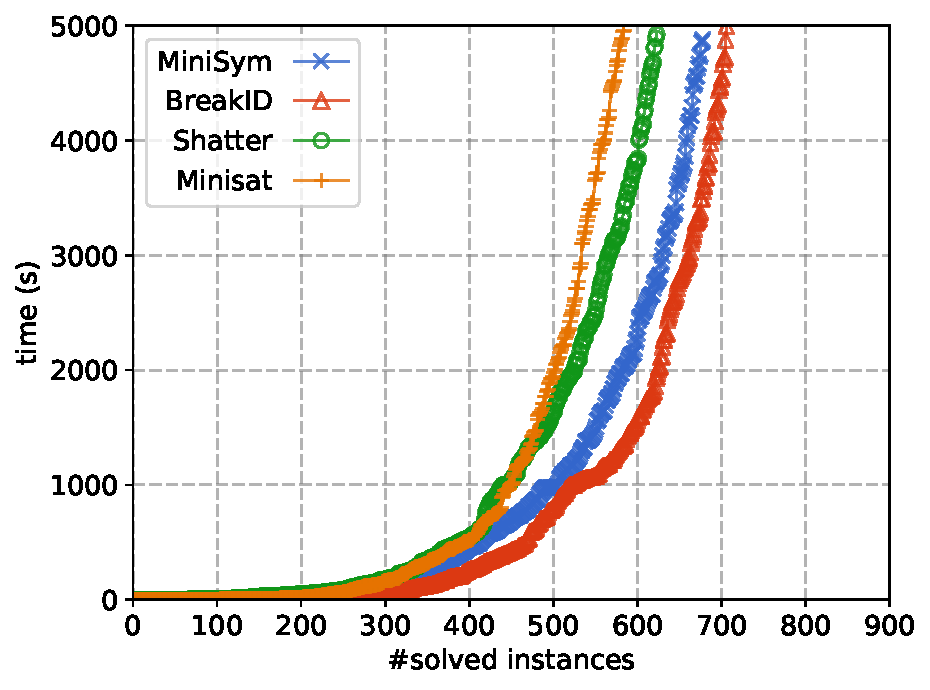
\includegraphics[scale=0.3]{images/saucy-result}}}%
%\hfill
%\subfloat[with \bliss]{
	{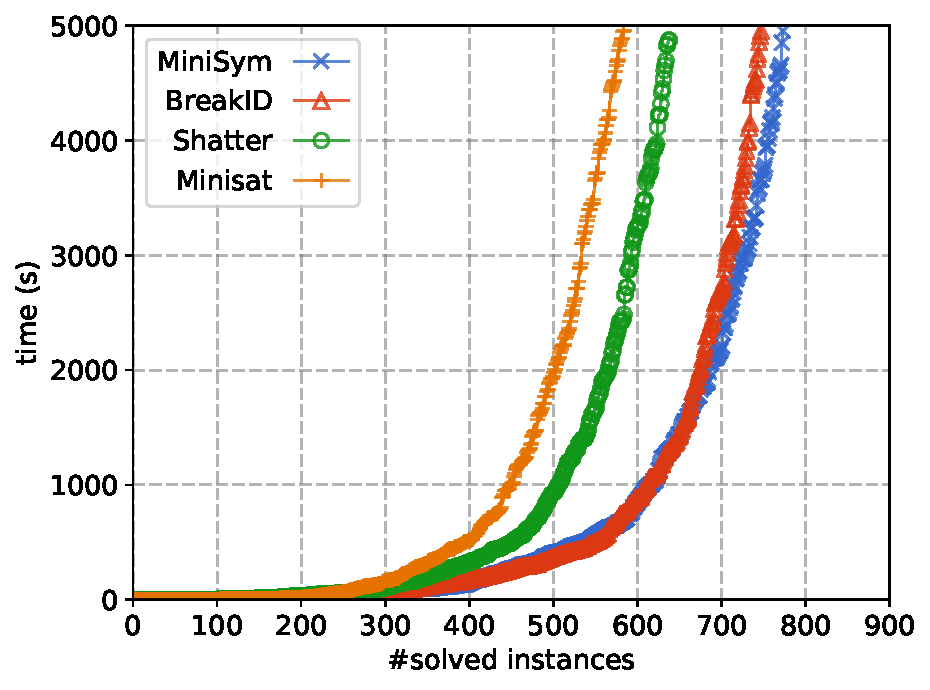
\includegraphics[scale=0.45]{images/bliss-result}}
%}%
\label{fig:cactus}%
\end{figure}

%\vspace{-0.3cm}
\begin{table}
%\resizebox{.75\textwidth}{!}{
%	\subfloat{%
%		\begin{tabular}{l|ccccc}
%			&\texttt{MiniSAT} & \texttt{Shatter} & \texttt{BreakID} & \texttt{MiniSym}\\
%			\midrule
%			PAR-2 sum  & 8\,074\,348 & 7\,770\,434 & \cellcolor{gray!30}\textbf{6\,909\,999} & 7\,229\,700\\
%			PAR-2 avg  & 5\,981 & 5\,756 & \cellcolor{gray!30}\textbf{5\,119} & 5\,355\\
%
%		\end{tabular}
%	}
%	\hspace{1em}
%	\subfloat{%
%
%\begin{tabular}{lcccc}
%	Solver & PAR-2 & ALL & SAT & UNSAT\\
%	\toprule
%	\textcolor{orange}{\texttt{MiniSAT}} & 2243h & 586 &325 &261 \\
%	\textcolor{green}{\texttt{Shatter}} &2088h & 640 & 316 &324 \\
%	\textcolor{red}{\texttt{BreakID}} &1790h & 749 &334 &415 \\
%	\textcolor{blue}{\textbf{\texttt{MiniSym}}} &  \cellcolor{gray!30}\textbf{1735h} &  \cellcolor{gray!30}\textbf{775} & \cellcolor{gray!30}\textbf{336} &  \cellcolor{gray!30}\textbf{439} \\
%	
%\end{tabular}

\only<1>{
\begin{tabular}{lccc}
	Solver & PAR-2  & SAT & UNSAT\\
	\toprule
	\textcolor{orange}{\texttt{MiniSAT}} & 2243h  &325 &261 \\
	\textcolor{green}{\texttt{Shatter}} &2088h  & 316 &324 \\
	\textcolor{red}{\texttt{BreakID}} &1790h  &334 &415 \\
	\textcolor{blue}{\textbf{\texttt{MiniSym}}} &  \cellcolor{gray!30}\textbf{1735h} & \cellcolor{gray!30}\textbf{336} &  \cellcolor{gray!30}\textbf{439} \\
\end{tabular}
}
\only<2>{
\begin{tabular}{l|c|c}
	Number of SBPs & \texttt{BreakID}  & \texttt{MiniSym}\\
	\hline
	\unsat (399)	&  2\,576\,349 &  \cellcolor{gray!30}\textbf{913\,339}\\
	\sat  (320) & 12\,179\,513  & \  \cellcolor{gray!30}\textbf{457\,452} 
	\label{sbp-bliss}
\end{tabular}
}
%		\begin{tabular}{l|ccccc}
%			&\texttt{MiniSAT} & \texttt{Shatter} & \texttt{BreakID} & \texttt{MiniSym}\\
%			\hline
%			PAR-2 sum & 8\,074\,348 & 7\,517\,556 & 6\,444\,954 & \cellcolor{gray!30}\textbf{6\,245\,448}\\
%			PAR-2 avg  & 5\,981 & 5\,569 & 4\,774 & \cellcolor{gray!30}\textbf{4\,626}\\
%		\end{tabular}
%	}
%}
%\vspace*{0.1cm}
%\caption{Time comparison}
\end{table}

\end{frame}

\begin{frame}
	\frametitle{Discussion of the results}
	
	Change the ordering relation
		\begin{itemize}
				\item Choose another lex-leader
				\item Generate other SBP
		\end{itemize}
	\vfill
	\visible<2->{
	 Composing permutations
		\begin{itemize}
			\item Observe more variables
			\item Earlier generation of ESBP 
		\end{itemize}
	}
\vfill
	\visible<3->{
	Adapt the solver heuristics dynamically
	\begin{itemize}
		\item Restart
		\item Cleaning database
	\end{itemize}
}
\end{frame}

\begin{frame}
\centering
\textcolor{UPMCEngagementBlueB}{\Large Exploitation of symmetries:}\\
\vspace{2em}
\textcolor{UPMCEngagementBlueB}{\Large Dynamic symmetry breaking}
\end{frame}




%\begin{frame}{Experimental results (\unsat versus \sat)}
%
%\begin{tabular}{lcccc}
%	Solver & PAR-2 & ALL & SAT & UNSAT\\
%	\toprule
%	\texttt{MiniSAT} & 2243h & 586 &325 &261 \\
%	\texttt{Shatter} &2088h & 640 & 316 &324 \\
%	\texttt{BreakID} &1790h & 749 &334 &415 \\
%    \texttt{MiniSym} &  \cellcolor{gray!30}\textbf{1735h} &  \cellcolor{gray!30}\textbf{775} & \cellcolor{gray!30}\textbf{336} &  \cellcolor{gray!30}\textbf{439} \\
%
%\end{tabular}
%
%
%\begin{table}[h!]
%\resizebox{1 \textwidth}{!}{
%\subfloat[With \saucy]{%
%	\begin{tabular}{l|ccccc}
%		&\texttt{MiniSAT} & \texttt{Shatter} & \texttt{BreakID} & \texttt{MiniSym}\\
%		\midrule
%		TOTAL   & 261 & 302 & \cellcolor{gray!30}\textbf{371} & 345\\
%	\end{tabular}
%}
%\hspace{1em}
%\subfloat[With \bliss]{%
%	\begin{tabular}{l|ccccc}
%		&\texttt{MiniSAT} & \texttt{Shatter} & \texttt{BreakID} & \texttt{MiniSym}\\
%		\midrule
%		TOTAL  & 261 & 324 & 415 & \cellcolor{gray!30}\textbf{439}\\
%	\end{tabular}
%}
%}
%\caption{Comparison on \unsat instances}
%\label{table:benchUNSAT}
%\end{table}
%\begin{table}
%\resizebox{1 \textwidth}{!}{
%\subfloat[With \saucy]{%
%	\begin{tabular}{l|ccccc}
%		&\texttt{MiniSAT} & \texttt{Shatter} & \texttt{BreakID} & \texttt{MiniSym}\\
%		\midrule
%		TOTAL  & 325 & 323 & \cellcolor{gray!30}\textbf{337} & 335\\
%
%	\end{tabular}
%}
%\hspace{1em}
%\subfloat[With \bliss]{%
%	\begin{tabular}{l|ccccc}
%		&\texttt{MiniSAT} & \texttt{Shatter} & \texttt{BreakID} & \texttt{MiniSym}\\
%		\hline
%		TOTAL & 325 & 316 & 334 & \cellcolor{gray!30}\textbf{336}\\
%	\end{tabular}
%}
%}
%\vspace*{0.1cm}
%\caption{Comparison on \sat instances}
%\end{table}
%\end{frame}

%% ----------------------------------------------------------------------------

\begin{frame}
	\frametitle{Learn symmetrical clauses}
	
	\begin{columns}[t]
		\begin{column}[T]{.3\textwidth}
			\begin{tabular}{cl}
				\begin{tikzpicture}
				\node[draw,thick, scale=0.5] at (0,0){};
				\end{tikzpicture} & formula  \\
				
				\begin{tikzpicture}
				\node[] at (0,0){$\omega$};
				\end{tikzpicture} & clause \\
				\visible<2->{
					\begin{tikzpicture}
					\node[] at (0,0){ \textcolor{orange}{$\omega$}};
					\end{tikzpicture} & \textcolor{orange}{learnt clause} \\
				}
				
			\end{tabular}
		\end{column}
		\begin{column}[T]{0.6\textwidth}
			\begin{tikzpicture}
			
			
			\tikzstyle{class1}=[draw, minimum width=6cm, minimum height=5cm]
			Our contribution C
			\node[] (p1) at (0, 0){$\omega_1$};
			\node[] (p2) at (1, 0){$\omega_2$};
			\node[] (p3) at (-2, -1){$\omega_3$};
			\node[] (p4) at (-3, -1){$\omega_4$};

			\node[] (p5) at (-1.7, 0.5){$\omega_5$};
			
			\node[] (p6) at (-2, 1.5){$\omega_6$};
			
			\node[] (p6) at (-1.5, 1.69){$\omega_7$};
			
			\node[] (p6) at (-1.15, 1.12){$\omega_8$};
			
			\node[] (p6) at (-2, 2.1){$\omega_9$};
			
			\node[,opacity=0, onslide={<3->,opacity=1}] (p7) at (0.5, -1.5){\textcolor{orange}{$g_1.\omega_{13}$}};
			
			\node[,opacity=0, onslide={<3->,opacity=1}] (pl) at (0.5, 1.5){\textcolor{orange}{$g_2.\omega_{13}$}};
			
			\node[] (p7a) at (0.9, -0.87){$\omega_{11}$};
			
			\node[] (p8) at (-1, 2){$\omega_{12}$};
			
			\node[] (po) at (-3 , -0.2){$\omega_{10}$};
			
			\node[,opacity=0, onslide={<2->,opacity=1}] (l) at (-1, 0.1){\textcolor{orange}{$\omega_{13}$}};
			
			
			
			\node[thick, draw, minimum width=6cm, minimum height=5cm] (c4) at (-1, 0) {};
			
			\draw[->,opacity=0, onslide={<3->,opacity=1}] (l) to [bend right=30] node [midway, left, align=center,opacity=0, onslide={<3->,opacity=1}] {$g_1$}  (p7);
			
			\draw[->,opacity=0, onslide={<3->,opacity=1}] (l) to [bend right=30] node [midway, left, align=center,opacity=0, onslide={<3->,opacity=1}] {$g_2$}  (pl);
			\draw[->,opacity=0, onslide={<3->,opacity=1}] (l) to [bend right=10] node [midway, fill=white, align=center,opacity=0, onslide={<3->,opacity=1}] {$g_3$}  (po);
			
			\end{tikzpicture}
		\end{column}
	\end{columns}
	
	
	\vfill
	
	\visible<2->{
		Learnt clauses are logical consequences of the formula\\
	}
	\visible<3>{
		\vfill
		$g \in G$ are symmetries of the formula \\$\rightarrow$ symmetrical learnt clauses are logical consequences too
	}

\end{frame}


%% ----------------------------------------------------------------------------
\begin{frame}
\frametitle{Using symmetries to accelerate the tree traversal}
\only<1-2>{$g = (x_1 \enskip x_2)(x_4 \enskip x_5)(x_7 \enskip x_8) $\\}
\only<3>{$g = (x_1 \enskip x_2)\textcolor{red!70}{(x_4 \enskip x_5)}(x_7 \enskip x_8) $\\}
\centering
\begin{tikzpicture}[scale=1, every node/.style={scale=1}]

\newcommand{\x}{2.07}
\newcommand{\y}{-1.5}
\tikzstyle{highlight} = [line width=0.3mm, color=blue]
\tikzstyle{decision}=[circle,draw,thick,fill=blue!30,font=\scriptsize]
%	\tikzstyle{unsat}=[draw,thick, fill=red]
\tikzstyle{unsat}=[scale=2, fill=white]
\tikzstyle{link}=[->,>=latex,rounded corners=5pt,thick]
\tikzstyle{transparent} = [nearly transparent]
\tikzstyle{mid}=[midway,fill=white,nearly transparent,opacity=1, text opacity=1,font=\scriptsize]
\tikzstyle{trmid}=[midway,fill=white,nearly transparent,opacity=1, text opacity=0.3,font=\scriptsize]
\tikzstyle{propagation}=[rectangle, minimum height=.65cm, minimum width=.65cm,draw,thick,fill=blue!15,font=\scriptsize,anchor=base]

% layer 1
\node[decision](t) at (0,0) {$x_1$};

% layer 2
\node[decision,transparent,onslide={<2->,opacity=1}](l) at (-\x,\y) {$x_2$};
\node[decision,transparent](r) at (\x,\y) {$x_2$};


% layer 3
\node[decision,transparent](ll) at (-\x-\x*0.5,2*\y) {$x_4$};
\node[propagation,transparent,onslide={<2->,opacity=1}](lr) at (-\x+\x*0.5,2*\y) {$x_4$};
\node[decision,transparent](rl) at (\x-\x*0.5,2*\y) {$x_4$};
\node[decision,transparent](rr) at (\x+\x*0.5,2*\y) {$x_4$};

% layer 4
\node[decision,transparent](lll) at (-\x-\x*0.5-\x*0.25,3*\y) {$x_5$};
\node[decision,transparent](llr) at (-\x-\x*0.5+\x*0.25,3*\y) {$x_5$};
\node[decision,transparent,onslide={<3>, propagation,fill=red!30,opacity=1}](lrl) at (-\x+\x*0.5-\x*0.25,3*\y) {$x_5$};
\node[decision,transparent](lrr) at (-\x+\x*0.5+\x*0.25,3*\y) {$x_5$};
\node[decision,transparent](rll) at (\x-\x*0.5-\x*0.25,3*\y) {$x_5$};
\node[decision,transparent](rlr) at (\x-\x*0.5+\x*0.25,3*\y) {$x_5$};
\node[decision,transparent](rrl) at (\x+\x*0.5-\x*0.25,3*\y) {$x_5$};
\node[decision,transparent](rrr) at (\x+\x*0.5+\x*0.25,3*\y) {$x_5$};

% layer 5
\node[unsat,transparent](llll) at (-\x-\x*0.5-\x*0.25-\x*0.125,4*\y) {\pgfuseplotmark{triangle}};
\node[unsat,transparent](lllr) at (-\x-\x*0.5-\x*0.25+\x*0.125,4*\y) {\pgfuseplotmark{triangle}};
\node[unsat,transparent](llrl) at (-\x-\x*0.5+\x*0.25-\x*0.125,4*\y) {\pgfuseplotmark{triangle}};
\node[unsat,transparent](llrr) at (-\x-\x*0.5+\x*0.25+\x*0.125,4*\y) {\pgfuseplotmark{triangle}};
\node[unsat,transparent](lrll) at (-\x+\x*0.5-\x*0.25-\x*0.125,4*\y) {\pgfuseplotmark{triangle}};
\node[unsat,transparent](lrlr) at (-\x+\x*0.5-\x*0.25+\x*0.125,4*\y) {\pgfuseplotmark{triangle}};
\node[unsat,transparent](lrrl) at (-\x+\x*0.5+\x*0.25-\x*0.125,4*\y) {\pgfuseplotmark{triangle}};
\node[unsat,transparent](lrrr) at (-\x+\x*0.5+\x*0.25+\x*0.125,4*\y) {\pgfuseplotmark{triangle}};
\node[unsat,transparent](rlll) at (\x-\x*0.5-\x*0.25-\x*0.125,4*\y) {\pgfuseplotmark{triangle}};
\node[unsat,transparent](rllr) at (\x-\x*0.5-\x*0.25+\x*0.125,4*\y) {\pgfuseplotmark{triangle}};
\node[unsat,transparent](rlrl) at (\x-\x*0.5+\x*0.25-\x*0.125,4*\y) {\pgfuseplotmark{triangle}};
\node[unsat,transparent](rlrr) at (\x-\x*0.5+\x*0.25+\x*0.125,4*\y) {\pgfuseplotmark{triangle}};
\node[unsat,transparent](rrll) at (\x+\x*0.5-\x*0.25-\x*0.125,4*\y) {\pgfuseplotmark{triangle}};
\node[unsat,transparent](rrlr) at (\x+\x*0.5-\x*0.25+\x*0.125,4*\y) {\pgfuseplotmark{triangle}};
\node[unsat,transparent](rrrl) at (\x+\x*0.5+\x*0.25-\x*0.125,4*\y) {\pgfuseplotmark{triangle}};
\node[unsat,transparent](rrrr) at (\x+\x*0.5+\x*0.25+\x*0.125,4*\y) {\pgfuseplotmark{triangle}};


\draw[link] (t) ->  node [mid] {$0$} (l);
\draw[link,transparent] (t) -> node [trmid] {$1$} (r);

\draw[link,transparent] (l) ->  node [trmid] {$0$} (ll);
\draw[link,transparent,onslide={<2->,opacity=1}] (l) -> node [trmid,onslide={<2->,mid}] {$1$} (lr);
\draw[link,transparent] (r) ->  node [trmid] {$0$} (rl);
\draw[link,transparent] (r) -> node [trmid] {$1$} (rr);

\draw[link,transparent] (ll) -> node [trmid] {$0$} (lll);
\draw[link,transparent] (ll) -> node [trmid] {$1$} (llr);
\draw[link,transparent,onslide={<2->,opacity=1}] (lr) -> node [trmid,onslide={<2->,mid}] {$0$} (lrl);
\draw[link,transparent] (lr) -> node [trmid] {$1$} (lrr);

\draw[link,transparent] (rl) -> node [trmid] {$0$} (rll);
\draw[link,transparent] (rl) -> node [trmid] {$1$} (rlr);
\draw[link,transparent] (rr) -> node [trmid] {$0$} (rrl);
\draw[link,transparent] (rr) -> node [trmid] {$1$} (rrr);


\draw[link,transparent] (lll) -> node [trmid] {$0$} (llll);
\draw[link,transparent] (lll) -> node [trmid] {$1$} (lllr);
\draw[link,transparent] (llr) -> node [trmid] {$0$} (llrl);
\draw[link,transparent] (llr) -> node [trmid] {$1$} (llrr);
\draw[link,transparent,onslide={<3->,opacity=1}] (lrl) -> node [trmid,onslide={<3->,mid}] {$0$} (lrll);
\draw[link,transparent] (lrl) -> node [trmid] {$1$} (lrlr);
\draw[link,transparent] (lrr) -> node [trmid] {$0$} (lrrl);
\draw[link,transparent] (lrr) -> node [trmid] {$1$} (lrrr);

\draw[link,transparent] (rll) -> node [trmid] {$0$} (rlll);
\draw[link,transparent] (rll) -> node [trmid] {$1$} (rllr);
\draw[link,transparent] (rlr) -> node [trmid] {$0$} (rlrl);
\draw[link,transparent] (rlr) -> node [trmid] {$1$} (rlrr);
\draw[link,transparent] (rrl) -> node [trmid] {$0$} (rrll);
\draw[link,transparent] (rrl) -> node [trmid] {$1$} (rrlr);
\draw[link,transparent] (rrr) -> node [trmid] {$0$} (rrrl);
\draw[link,transparent] (rrr) -> node [trmid] {$1$} (rrrr);
\end{tikzpicture}
\vfill
\visible<3> {Use symmetries to deduce symmetrical facts.}
\end{frame}



\begin{frame}
\frametitle{State-of-the-art dynamic symmetry breaking}
State-of-the-art:
\begin{itemize}
	\item Symmchaff~\cite{sabharwal2005symchaff}
	\item Symmetry Learning Scheme (SLS)~\cite{benhamou2010enhancing}
	\item Symmetry Propagation (SP)~\cite{Devriendt12}
	\item Symmetry Explanation Learning (SEL)~\cite{devriendt2017symmetric}
\end{itemize}

\vfill
\begin{center}
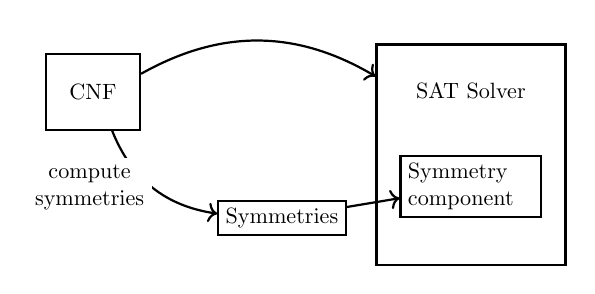
\begin{tikzpicture}[scale=0.8,every node/.style={scale=0.8}]
\tikzstyle{box} = [draw, minimum width=1.5cm]

\node[box,thick,minimum height=1.2cm] (cnf) at (-5, 0) {CNF};
\node[box,thick] (sym) at (-2, -2) { Symmetries};


\node[box,thick,minimum width=3cm,minimum height=3.5cm,label={[yshift=-1cm]SAT Solver}] (solver) at (1, -1) { };
\node[box,thick,text width=2cm] (symcomp) at (1, -1.5) {Symmetry component};
\draw[->, thick, bend left = 30] (cnf) to [bend right=30] node [midway, left, fill=white, align=center] {compute\\symmetries} (sym);

\draw[->, thick,bend left = 30] (cnf) to [] (solver);
\draw[->, thick] (sym) to [] (symcomp);
\end{tikzpicture}
\end{center}
\vfill


\visible<2>{
%Pros/Cons:
%\begin{itemize}
%	\item \textcolor{hgreen}{Works well on many symmetric instances}
%	\item \textcolor{red}{Cannot handle some instances solved by static approach}
%\end{itemize}

Observations:\\
 
\textcolor{green}{Solve some instances very quicly}\\
\textcolor{orange}{Cannot handle some instances solved by static approach}
}

\end{frame}


%% ----------------------------------------------------------------------------

%\begin{frame}
%\frametitle{Example}
%TODO\\
%Build an example
%\end{frame}
%% ----------------------------------------------------------------------------
%
%\begin{frame}
%\frametitle{Outline}
%\begin{enumerate}
%\item \textcolor{UPMCEngagementBlueB}{SAT overview}
%\begin{itemize}
%\item[] SAT basics
%\item[] SAT and symmetries
%\end{itemize}
%\vspace{5pt}
%\item \textcolor{UPMCEngagementBlueB}{Existing approaches}
%\begin{itemize}
%\item[] Static symmetry breaking
%\item[] Dynamic symmetry breaking
%\end{itemize}
%\vspace{5pt}
%\item \textcolor{UPMCEngagementBlueB}{Contribution and results}
%\begin{itemize}
%\item[] CDCL [Sym]
%\item[] Combination of different approaches
%\end{itemize}
%\end{enumerate}
%\end{frame}
%

\begin{frame}
	\centering
	\textcolor{UPMCEngagementBlueB}{\Large Second contribution }\\
	\vspace{2em}
	\textcolor{UPMCEngagementBlueB}{\Large Composing Symmetry Propagation and Effective Symmetry Breaking for SAT Solving }\\
	\vspace{2em}
	\textcolor{UPMCEngagementBlueB}{\Large  NFM'19~\cite{metin2019composing}}
\end{frame}


\begin{frame}
\frametitle{Composing ESBP and SP}


Compose the symmetry propagation and the ESBP\\
\begin{center}
	\textit{prune the decision tree while accelerating its traversal}
\end{center}

\vfill

Problems:
\begin{itemize}
	\item ESBP breaks symmetries (incrementally)
	\item SP considers the manipulated symmetries valid all time
\end{itemize}

\vfill
\centering
In a hybrid approach, SP must be able to identify\\ \textbf{valid symmetries}
\end{frame}
%% ----------------------------------------------------------------------------


\begin{frame}
	\frametitle{Is valid symmetry?}
	
	Our proposal: Local symmetries
	
	\vfill
	
	Consider the symmetry at clause level instead of formula level
	
	\vfill
	
	\begin{center}
		\textbf{Guarantee that symmetrical clauses are logical consequences of the formula}
	\end{center}
	
\end{frame}

\begin{frame}
	\frametitle{Local symmetry}
		\begin{columns}[t]
		\begin{column}[T]{.3\textwidth}
			\begin{tabular}{cl}
				\begin{tikzpicture}
				\node[draw,thick, scale=0.5] at (0,0){};
				\end{tikzpicture} & formula  \\
				
				\begin{tikzpicture}
				\node[] at (0,0){$\omega$};
				\end{tikzpicture} & clause \\
				\visible<1->{
					\begin{tikzpicture}
					\node[] at (0,0){ \textcolor{orange}{$\omega$}};
					\end{tikzpicture} & \textcolor{orange}{learnt clause} \\
				}
					\visible<2->{
					\begin{tikzpicture}
					\node[] at (0,0){ \textcolor{purple}{$\omega$}};
					\end{tikzpicture} & \textcolor{purple}{ESBP} \\
				}
			\end{tabular}
		\end{column}
		\begin{column}[T]{0.6\textwidth}
			
			\begin{tikzpicture}
			
			
			\tikzstyle{class1}=[draw, minimum width=6cm, minimum height=5cm]
			Our contribution C
			\node[] (p1) at (0, 0){$\omega_1$};

			
			\node[] (p2) at (1, 0){$\omega_2$};
			%	\node[](a5) at (1, 0.25) {$\alpha_5$};
			
			\node[] (p3) at (-2, -1){$\omega_3$};
			%	\node[](a6) at (-2, -0.75) {$\alpha_6$};
			
			\node[] (p4) at (-3, -1){$\omega_4$};
			%	\node[](a4) at (-3, -0.75) {$\alpha_4$};
			
			\node[] (p5) at (-1.7, 0.5){$\omega_5$};
			%	\node[](a1) at (-1.7, 0.75) {$\alpha_1$};
			
			\node[] (p6) at (-2, 1.5){$\omega_6$};
			
			\node[] (p6) at (-1.5, 1.69){$\omega_7$};
			
			\node[] (p6) at (-1.15, 1.12){$\omega_8$};
			
			\node[] (p6) at (-2, 2.1){$\omega_9$};
			%	\node[](a2) at (-2, 1.75) {$\alpha_2$};
			
			
			
			\node[,opacity=0, onslide={<5->,opacity=1}] (p7) at (0.5, -1.5){\textcolor{orange}{$g_1.\omega_{14}$}};
			
			%\node[,opacity=0, onslide={<4->,opacity=1}] (pl) at (0.5, 1.5){\textcolor{orange}{$\omega$}};
			
			\node[] (p7a) at (0.9, -0.87){$\omega_{11}$};
			%	\node[](a7) at (0.5, -1.25) {$\alpha_7$};
			
			\node[] (p8) at (-1, 2){$\omega_{12}$};
			
			\node[] (po) at (-3 , -0.2){$\omega_{10}$};
			%	\node[](a8) at (-1, 2.25) {$\alpha_8$};
			
			\node[,opacity=0, onslide={<5->,opacity=1}] (l) at (-0.85, 0.1){\textcolor{orange}{$\omega_{15}$}};
			
			\node[,opacity=0, onslide={<2->,opacity=1}] (lpp) at (-2.25, 0.8){\textcolor{purple}{$\omega_{13}$}};
			
			\node[,opacity=0, onslide={<4->,opacity=1}] (lpp2) at (1.55, 1.40){\textcolor{purple}{$\omega_{14}$}};
			\node[thick, draw, minimum width=6cm, minimum height=5cm] (c4) at (-1, 0) {};
			
			\draw[->,opacity=0, onslide={<5->,opacity=1}] (l) to [bend right=30] node [midway, left, align=center,opacity=0, onslide={<5->,opacity=1}] {$g_1$}  (p7);
			
		%	\draw[->,opacity=0, onslide={<3>,opacity=1}] (l) to [bend right=30] node [midway, left, align=center,opacity=0, onslide={<3>,opacity=1}] {$g_2$}  (pl);
			\draw[->,opacity=0, onslide={<5->,opacity=1}] (l) to [bend right=10] node [midway, fill=white, align=center,opacity=0, onslide={<5->,opacity=1}] {$g_3$}  (po);
			
			
				\draw[->,opacity=0, onslide={<3->,opacity=1}] (lpp)  to[out=90, in=180,loop,looseness=4.8]node [midway, left, align=center,opacity=0, onslide={<3->,opacity=1}] {$g_1, g_2$}  (lpp);
				
				\draw[->,opacity=0, onslide={<4->,opacity=1}] (lpp2)  to[out=90, in=180,loop,looseness=4.8]node [midway, left, align=center,opacity=0, onslide={<4->,opacity=1}] {$g_1, g_3$}  (lpp2);
				
			\end{tikzpicture}
		\end{column}
	\end{columns}

\vfill
\begin{columns}[t]
	\begin{column}[t]{.3\textwidth}
		Local symmetries:\\
		$\omega \leftarrow \{g_1, g_2, g_3\}$\\
		\visible<3->{\textcolor{purple}{$\omega_{13}$} $\leftarrow \{g_1, g_2 \}$}\\
		\visible<4->{\textcolor{purple}{$\omega_{14}$} $\leftarrow \{g_1, g_3 \}$}\\
		\visible<5->{\textcolor{orange}{$\omega_{15
				}$} $\leftarrow \{g_1, g_3\}$}
	\end{column}
\begin{column}[t]{.6\textwidth}
	\begin{itemize}
	\item \visible<3->{Compute valid local symmetries}\\
		\item \visible<3->{On the fly}\\
	\item \visible<3->{At minimal cost}\\
	\end{itemize}
	\centering \visible<5->{\textbf{Inductive construction}}
\end{column}
\end{columns}
\end{frame}

%\begin{frame}
%\frametitle{Local symmetries}
%  \begin{columns}[t]
%	\begin{column}[c]{.4\textwidth}
%		Formula $\leftarrow$ ($\{g_1, g_2, g_3\}$)
%	\end{column}
%	\begin{column}[t]{.5\textwidth}
%		\begin{itemize}
%			\item[] $\omega_1 \leftarrow$ ($\{g_1, g_2, g_3\}$)
%			\item[] $\omega_2 \leftarrow$ ($\{g_1, g_2, g_3\}$)
%			\item[] $\omega_3 \leftarrow$ ($\{g_1, g_2, g_3\}$)
%			\item[] $\omega_4 \leftarrow$ ($\{g_1, g_2, g_3\}$)
%			\smallskip
%			\visible<2->{\item[] $\omega_{5}$} \visible<3->{$\leftarrow$ ($\{g_1, g_3\}$)}
%		\end{itemize}
%\end{column}
%\end{columns}
%
%\vfill
%
%  \begin{columns}[t]
%	\begin{column}[c]{.3\textwidth}
%		Macro level
%	\end{column}
%	\begin{column}{.7\textwidth}
%		$\rightarrow \qquad$ Micro level
%	\end{column}
%\end{columns}
%
%\vfill
%\visible<3->{Compute valid local symmetries on-the-fly at a minimal cost.}
%\visible<4>{
%\begin{itemize}
%	\item Inductive construction of the valid symmetries
%	\item During the solving
%	\item At a minimal cost
%\end{itemize}
%}
%\end{frame}

%% ----------------------------------------------------------------------------

\begin{frame}
\frametitle{Experimental results}

\textbf{Benchmark:}
\begin{itemize}
	\item from SAT contests 2012 -- 2018
	\item filter: \bliss{} finds  symmetries in $1000$ seconds
	\item $1400$ symmetric instances (out of $4000$)
\end{itemize}

\vfill

\textbf{Setup:}
\begin{itemize}
	\item three tools
	\begin{itemize}
		\item  MiniSat SP (Minisat with Symmetry Propagation)
		\item  MiniSat ESBP (Minisat with cosy)
		\item  \textbf{Minisat ESBP-SP} (our approach)
	\end{itemize}
	\item $7200$ seconds timeout
\end{itemize}

\centering
%\resizebox{.7\textwidth}{!}{


%}
\end{frame}

%% ----------------------------------------------------------------------------

\begin{frame}{Experimental results}
%\begin{block}{}
%\centering 	$\bliss$ gives more generators than $\saucy$
%\end{block}

\begin{figure}[t]
	\centering
	{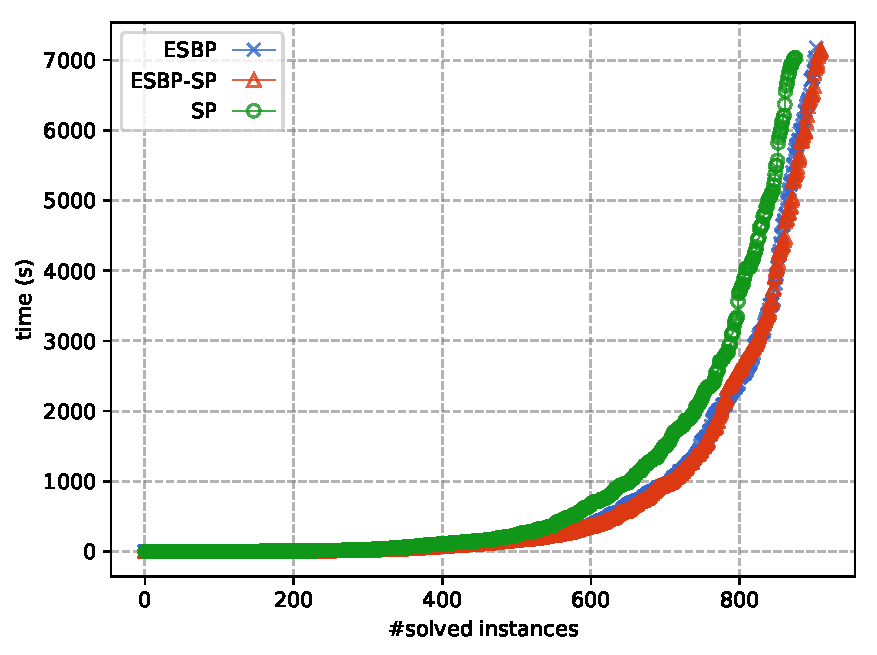
\includegraphics[scale=0.45]{images/combores2}}

\end{figure}
\centering

%\begin{tabular}{lcccc}
%	Solver & PAR-2 & ALL & SAT & UNSAT\\
%	\toprule
%	\textcolor{green}{SP} & 1674h00 & 876 & 406 & 470 \\
%	\textcolor{blue}{ESBP} & 1578h30 & 904 & 416 & 488\\
%	\textcolor{red}{\textbf{ESBP-SP}} & \cellcolor{gray!30}\textbf{1570h15} & \cellcolor{gray!30}\textbf{911} & \cellcolor{gray!30}\textbf{420} & \cellcolor{gray!30}\textbf{491}\\
%\end{tabular}
\begin{tabular}{lccc}
	Solver & PAR-2  & SAT & UNSAT\\
	\toprule
	\textcolor{green}{SP} & 1674h00  & 406 & 470 \\
	\textcolor{blue}{ESBP} & 1578h30  & 416 & 488\\
	\textcolor{red}{\textbf{ESBP-SP}} & \cellcolor{gray!30}\textbf{1570h15} &  \cellcolor{gray!30}\textbf{420} & \cellcolor{gray!30}\textbf{491}\\
\end{tabular}
\end{frame}

\begin{frame}
	\frametitle{Discussion of the results}
	
	SP and ESBP have separated symmetry  $\rightarrow$ costly
	
	\vfill
	\visible<2>{
	
	Combine ESBP with Symmetry Explanation Learning (SEL)
	\begin{itemize}
		\item SEL have less  requirements than SP
		\item We believe that this will improves the performance
	\end{itemize}
}
\end{frame}

\begin{frame}
\frametitle{Conclusion \& Perspectives}

	 Conclusion
	\begin{itemize}
	\item A new dynamic symmetry breaking approach
	\begin{itemize}
		\item Generation of SBP on the fly
		\item Package as a library $\libdsb$ usable with any CDCL solver
	\end{itemize}

	\item A new hybrid approach (ESBP-SP)
	\begin{itemize}
		\item Take advantage of static and dynamic approaches
	\end{itemize}
\end{itemize}
\vfill
\visible<3->{
 Perspectives
 \begin{itemize}
 	\item 	Exploitation of partial symmetries
 	\item 	Symmetries and parallel SAT solver
 \end{itemize}
}
\vfill
\flushright
\visible<4>{\textbf{Thanks !}}
\end{frame}
%% ----------------------------------------------------------------------------
%\begin{frame}
%\frametitle{Perspectives}
%\begin{itemize}
%	\item Combination of CDCL[Sym] with other dynamic symmetry breaking approach
%
%
%	\vfill
%	\item Combination with parallel SAT solver
%
%	\vfill
%	\item Exploitation of partial symmetries
%
%
%
%\end{itemize}
%
%\vfill
%\flushright
%\visible<2>{\textbf{Thanks !}}
%\end{frame}


%\begin{frame}
%\frametitle{Computing symmetries of a SAT problem}
%% \setlength{\tabcolsep}{35pt}
%
%\newcolumntype{C}{ >{\centering\arraybackslash} m{5cm} }
%\newcolumntype{D}{ >{\centering\arraybackslash} m{1cm} }
%\begin{tabular}{CC}
%	$CNF\ formula$ &{\scriptsize
%		\begin{tabular}{c}
%			$(x_1 \lor x_2 \lor x_3) \land
%			(x_4 \lor x_5 \lor x_6) \land
%			(x_7 \lor x_8 \lor x_9) $\\
%			$\land (\neg x_1 \lor \neg x_4) \land
%			(\neg x_1 \lor \neg x_7) \land
%			(\neg x_4 \lor \neg x_7)$\\
%			$\land (\neg x_2 \lor \neg x_5) \land
%			(\neg x_2 \lor \neg x_8) \land
%			(\neg x_5 \lor \neg x_8)$ \\
%			$\land (\neg x_3 \lor \neg x_6) \land
%			(\neg x_3 \lor \neg x_9) \land
%			(\neg x_6 \lor \neg x_9)$\\
%	\end{tabular}}\\
%	\only<2> {
%
%		$\Downarrow$ & $\Downarrow$  \\
%
%		colored graph &
%		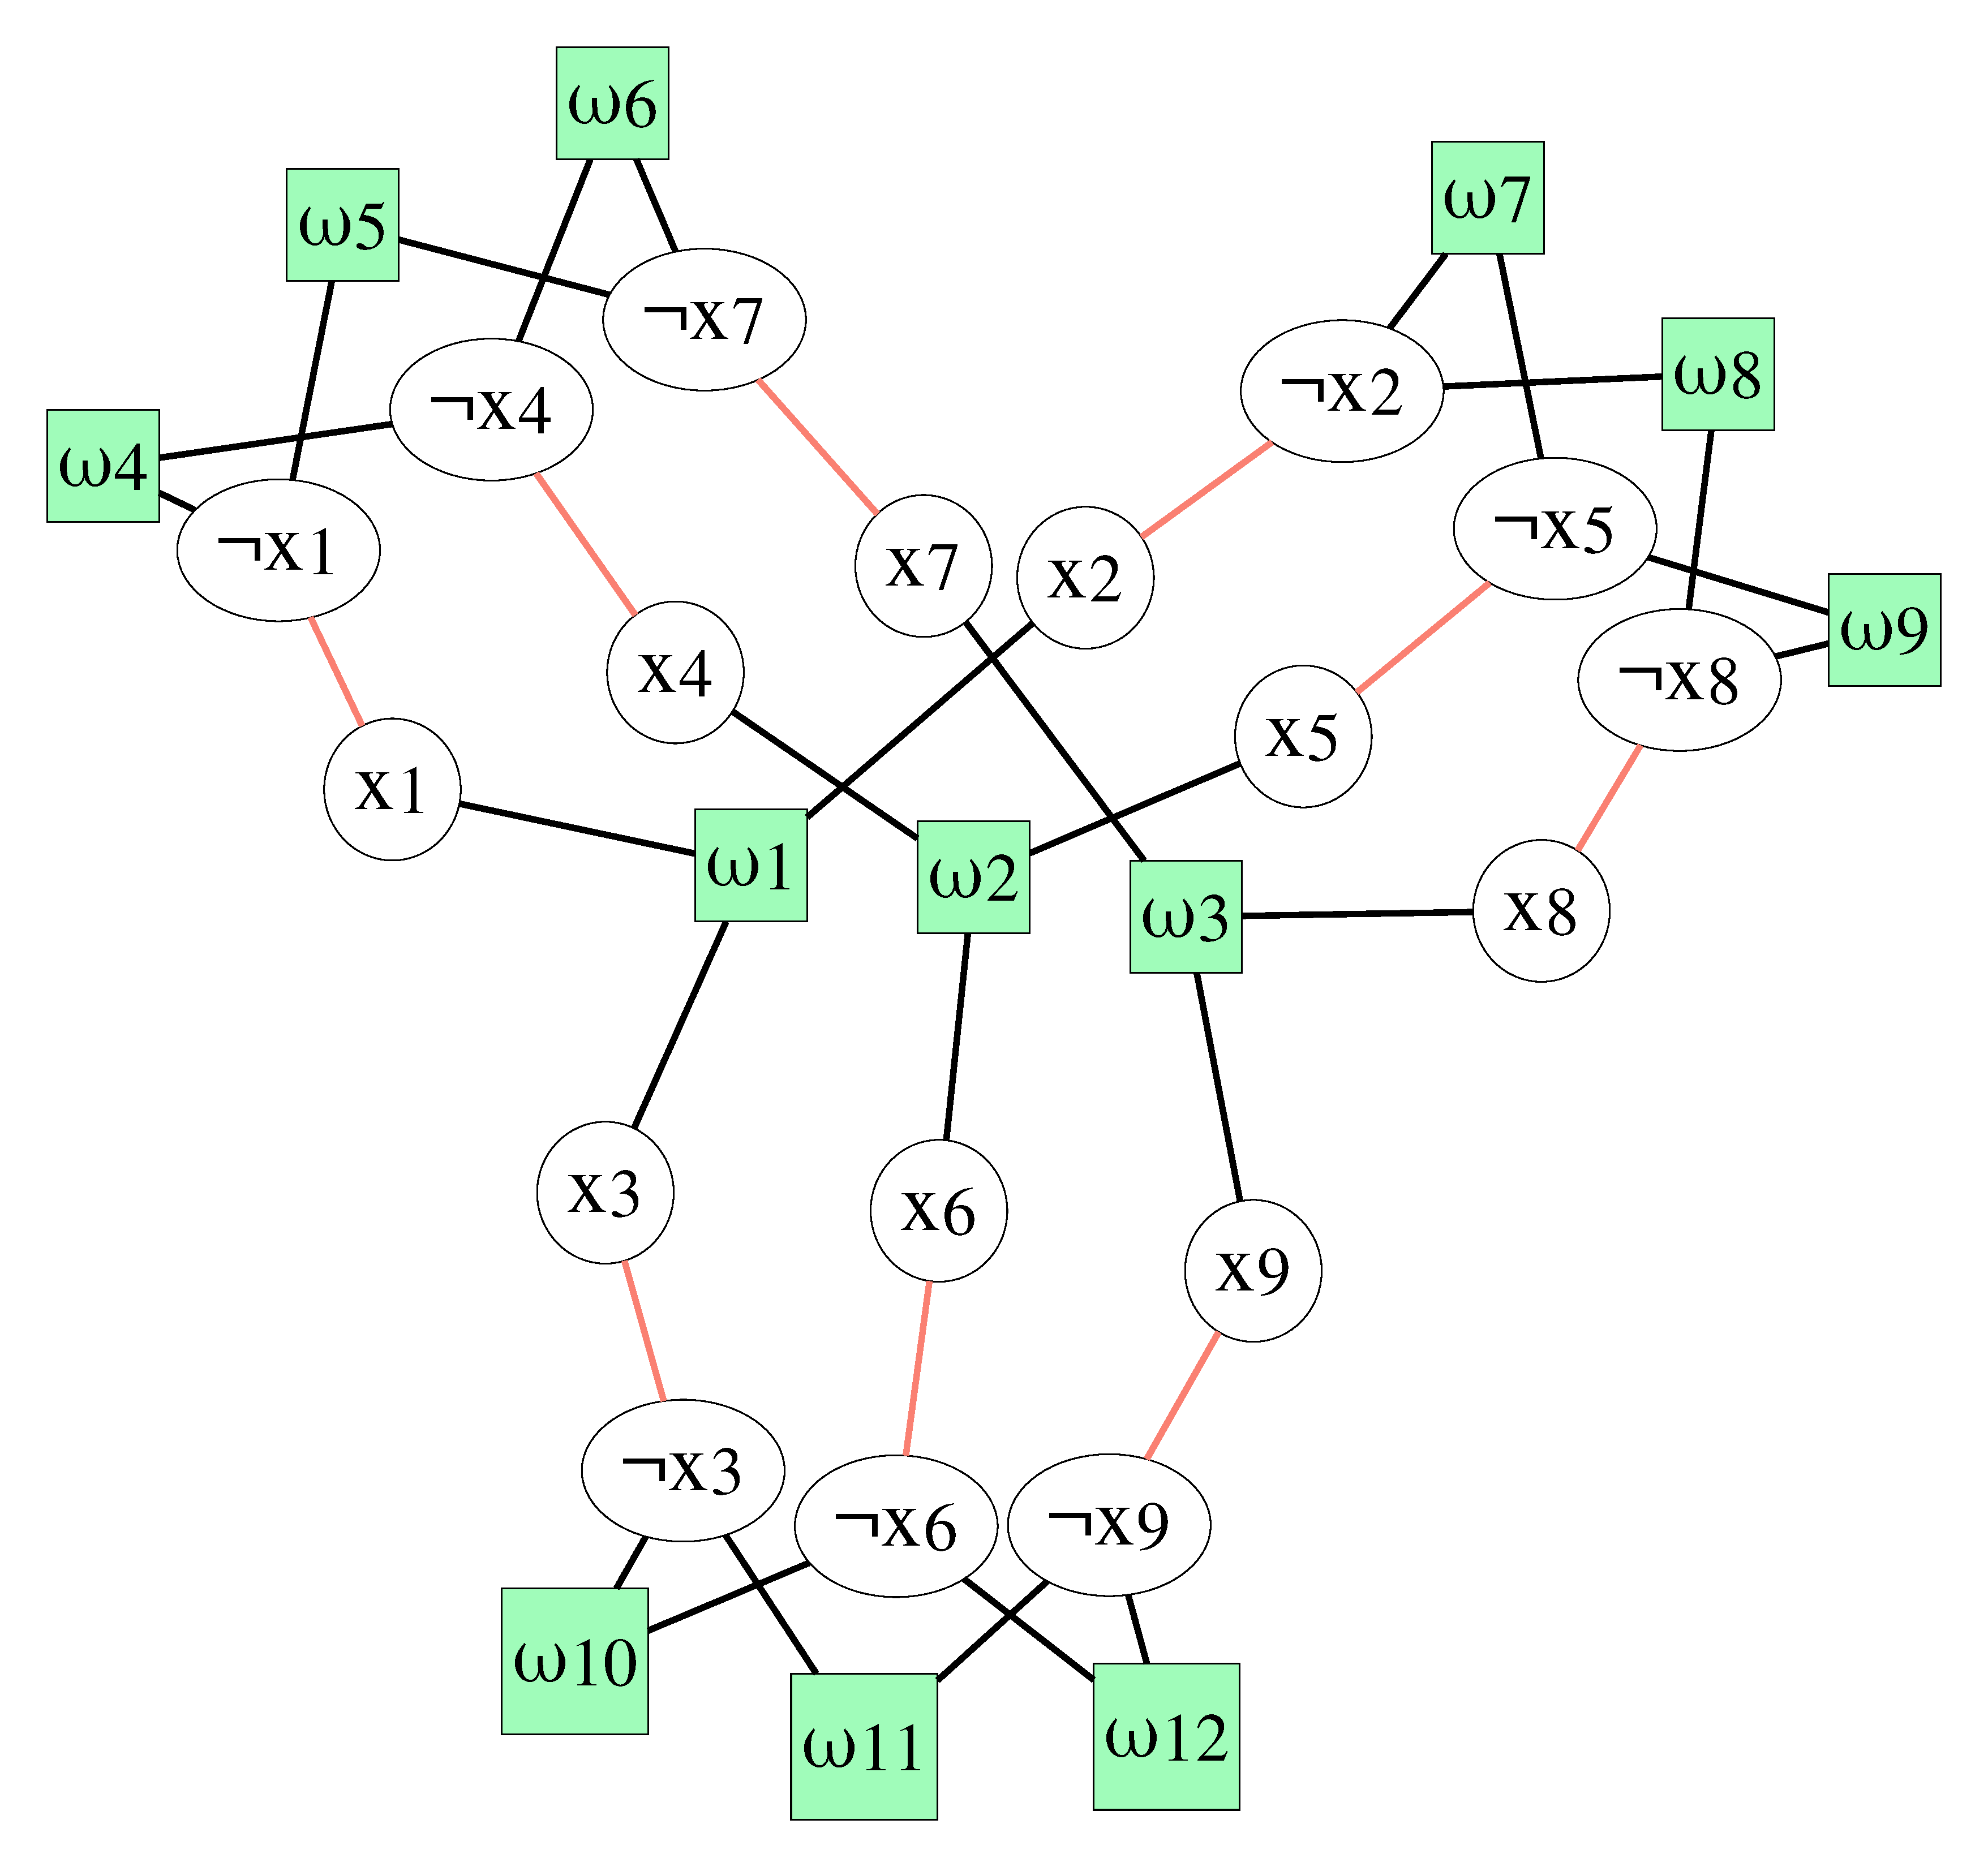
\includegraphics[scale=0.1]{images/graph}\\ \\
%	}
%
%	\visible<3-> {
%
%		$\Downarrow$ & $\Downarrow$  \\
%
%		colored graph &
%		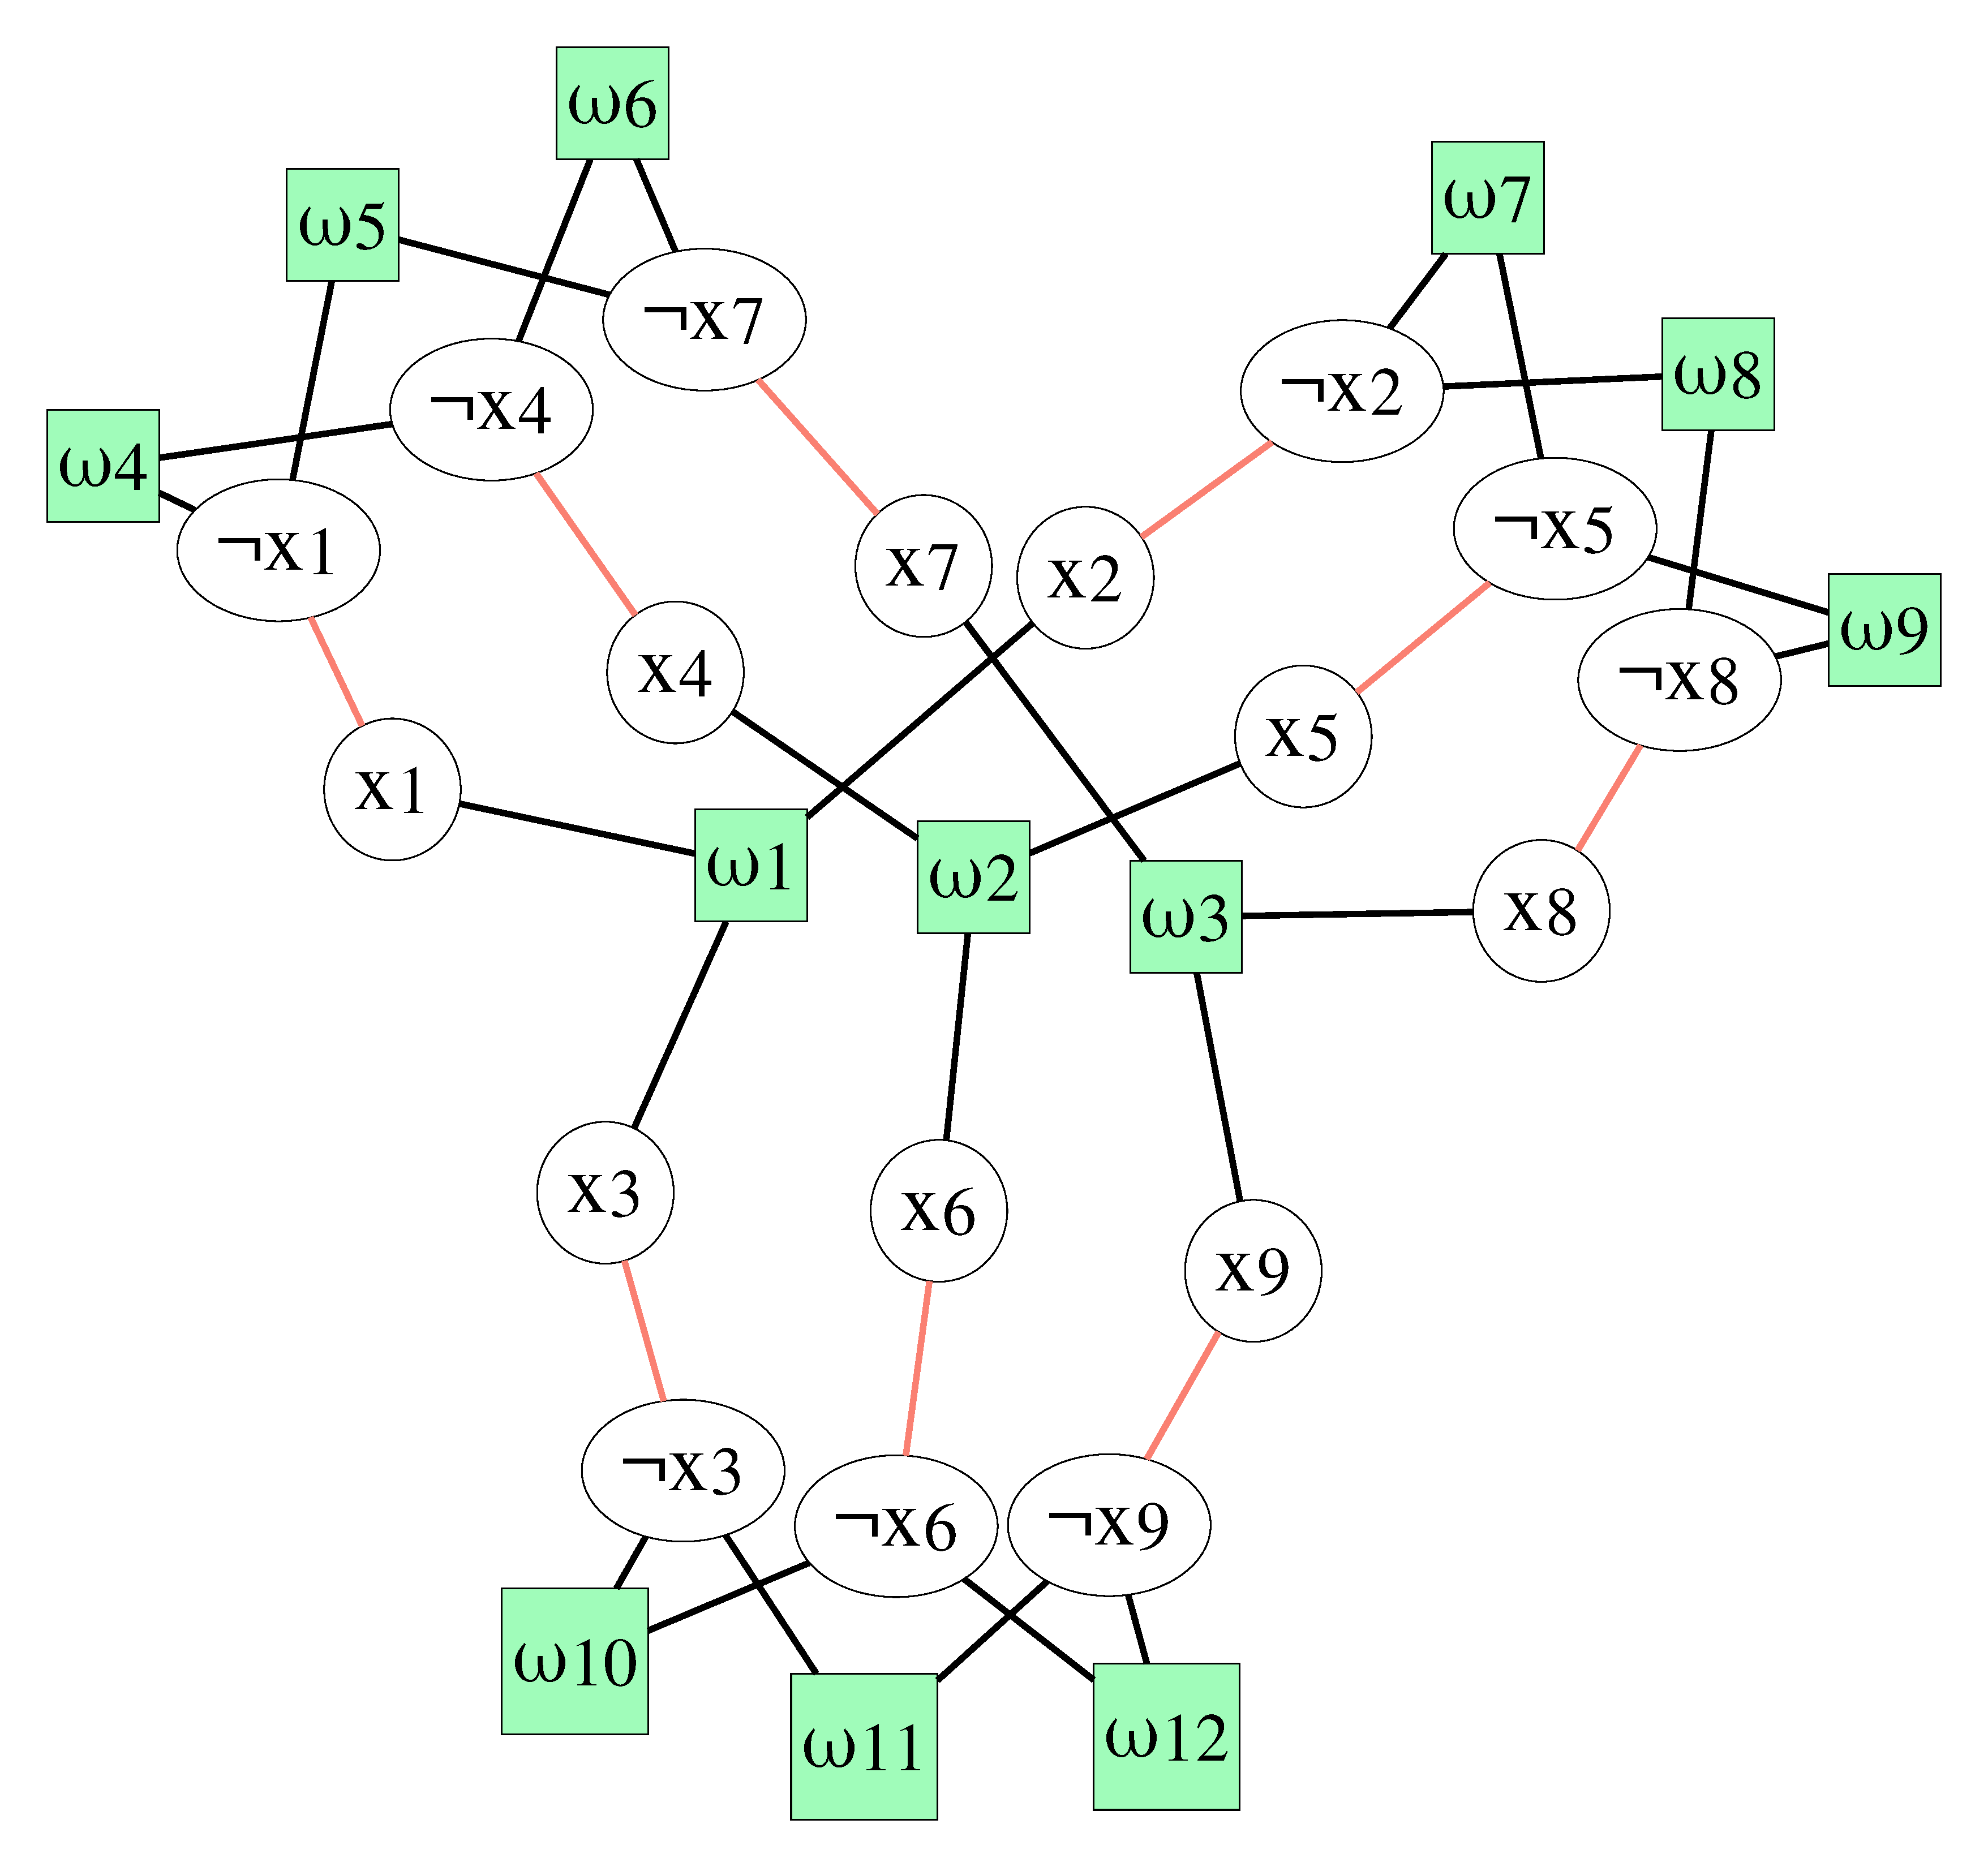
\includegraphics[scale=0.05]{images/graph}\\ \\
%	}
%	\visible<3-> {
%		$\|$ & $\|$  \\
%		graph automorphism &
%		\small{(\texttt{bliss} \footnote{http://www.tcs.hut.fi/Software/bliss/} or
%			\texttt{saucy} \footnote{http://vlsicad.eecs.umich.edu/BK/SAUCY/})}
%		\\
%	}
%
%
%	\visible<4-> {
%		$\Downarrow$ & $\Downarrow$  \\
%
%		set of symmetries & %\begin{frame}
%		%\tikzstyle{every picture}+=[remember picture]
%		%\frametitle{An UNSAT example}
%		%\everymath{\displaystyle}
%		%\centering
%		%
%		%\begin{tabular}{cc}
%		%	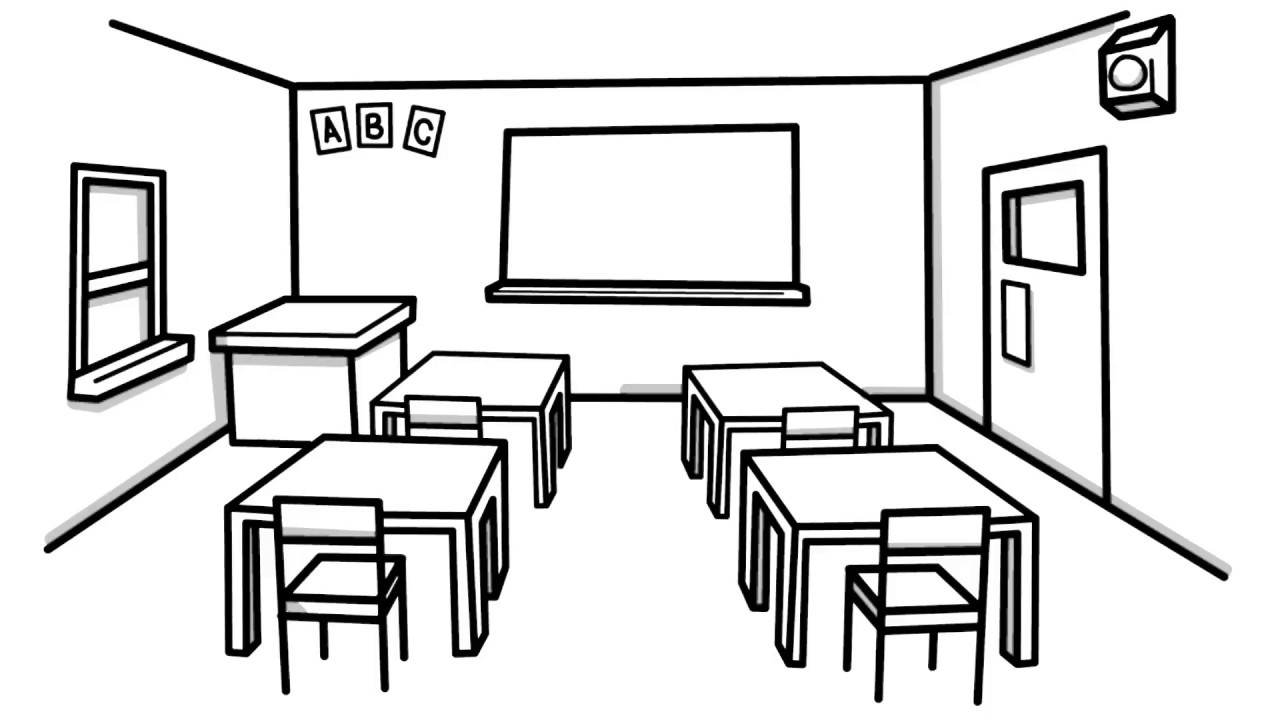
\includegraphics[scale=0.07]{images/room} & 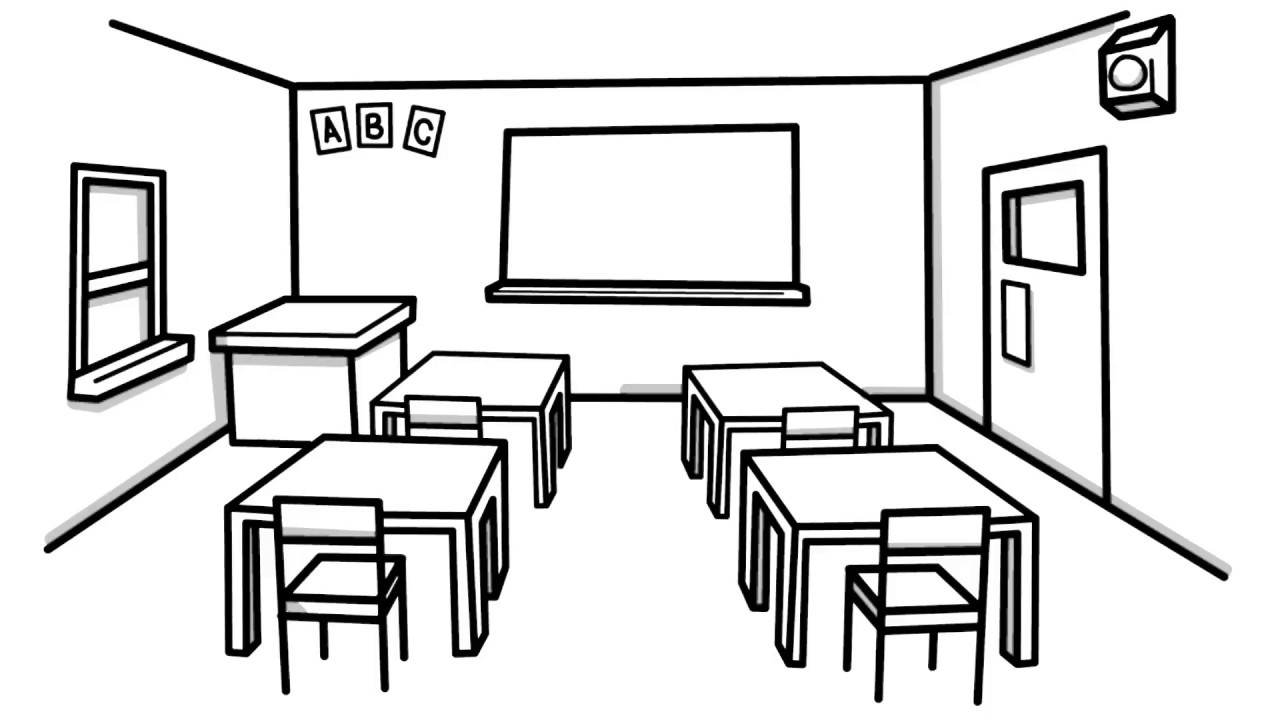
\includegraphics[scale=0.07]{images/room}\\
%		%	\tikz[baseline]{\node[anchor=base] (r1){1};} & \tikz[baseline]{\node[anchor=base] (r2){2};}\\
%		%\end{tabular}
%		%
%		%\begin{tabular}{ccc}
%		%	\tikz[baseline]{\node[anchor=base] (g1){};} & \tikz[baseline]{\node[anchor=base] (g2){};} & \tikz[baseline]{\node[anchor=base] (g3){};}\\
%		%	
\includegraphics[scale=0.1]{images/south} & 
\includegraphics[scale=0.1]{images/simpson} & 
\includegraphics[scale=0.09]{images/titeuf}\\
%		%	A                                        & B                                           & C\\
%		%\end{tabular}
%		%
%		%\visible<2->{
%		%	\begin{tikzpicture}[overlay]
%		%	\tikzstyle{line} = [<-, line width=0.5mm];
%		%	\path[line]<3> (r1) edge  (g1.south);
%		%	\path[line]<3> (r2) edge  (g2.south);
%		%
%		%	\path[line]<4> (r1) edge  (g2.south);
%		%	\path[line]<4> (r2) edge  (g1.south);
%		%
%		%	\path[line]<5> (r1) edge  (g1.south);
%		%	\path[line]<5> (r2) edge  (g3.south);
%		%
%		%	\path[line]<6> (r1) edge  (g3.south);
%		%	\path[line]<6> (r2) edge  (g1.south);
%		%
%		%	\path[line]<7> (r1) edge  (g2.south);
%		%	\path[line]<7> (r2) edge  (g3.south);
%		%
%		%	\path[line]<8> (r1) edge  (g3.south);
%		%	\path[line]<8> (r2) edge  (g2.south);
%		%
%		%	\visible<9>{
%		%	\node[draw, minimum width=3cm, minimum height=2cm,line width=0.5mm, color=orange](a) at (-1.75, 4.25) {};
%		%  	\node[draw, minimum width=3cm, minimum height=2cm,line width=0.5mm, color=orange](a) at (1.8, 4.25) {};
%		%
%		%	\node[draw, minimum width=3.5cm, minimum height=1.75cm,line width=0.5mm, color=blue](a) at (-3.5, 1.5) {};
%		%	\node[draw, minimum width=3.1cm, minimum height=1.75cm,line width=0.5mm, color=blue](a) at (0.25, 1.5) {};
%		%	\node[draw, minimum width=3.5cm, minimum height=1.75cm,line width=0.5mm, color=blue](a) at (3.9, 1.5) {};
%		%	}
%		%	\end{tikzpicture}
%		%}
%		%
%		%\vfill
%		%Is it possible to attribute each group to a classroom?\\
%		%\begin{center}
%		%	\visible<8->{No!}
%		%\end{center}
%		%
%		%\end{frame}
%		\scriptsize
%		\begin{tabular}{c}
%			$g_1 = (x_2 \enspace x_3)(x_5 \enspace x_6)(x_8 \enspace x_9)$\\
%			$g_2 = (x_4 \enspace x_7)(x_5 \enspace x_8)(x_6 \enspace x_9)$\\
%			$g_3 = (x_1 \enspace x_2)(x_4 \enspace x_5)(x_7 \enspace x_8)$\\
%			$g_4 = (x_1 \enspace x_4)(x_2 \enspace x_5)(x_3 \enspace x_6)$
%		\end{tabular}
%	}
%\end{tabular}
%\end{frame}



%% ----------------------------------------------------------------------------

\begin{frame}[allowframebreaks,noframenumbering]
  \scriptsize
%  \nocite{*}
  \bibliographystyle{alpha}
  \bibliography{main}
\end{frame}




\begin{frame}[noframenumbering]
\frametitle{Weakly active symmetries}

\begin{block}{Logical consequence}
	When $\omega$ is satisfied in all satisfying assignments of $\varphi$, we say that $\omega$ is a
	logical consequence of $\varphi$, and we denote this by $\varphi \vdash \omega$.
\end{block}

\visible<2->{
	\begin{block}{Weakly active symmetries}
		Let a subset $\delta \subseteq \alpha $, a symmetry $\sigma$ of $\varphi$ such that\\ $\varphi \cup \delta \vdash \varphi \cup \alpha \land \sigma.\delta \subseteq \alpha $ then $\sigma$ is weakly active symmetry.
	\end{block}
}

\visible<3->{
	\begin{block}{Symmetry propagation}
		Let $\sigma$ a weakly active symmetry, then
		$$ \varphi \cup \alpha  \vdash \{l\} \Leftrightarrow \varphi \cup \alpha  \vdash \sigma.\{l\}$$

	\end{block}
}
\end{frame}


\begin{frame}[noframenumbering]
\frametitle{Local symmetries}
\newcommand{\symm}[0]{\ensuremath{\mathfrak{S}}}

\begin{block}{Logical consequence}
	When $\omega$ is satisfied in all satisfying assignments of $\varphi$, we say that $\omega$ is a
	logical consequence of $\varphi$, and we denote this by $\varphi \vdash \omega$.
\end{block}

\begin{block}{Local Symmetries}
	Let $\varphi$ be a formula. We define $L_{\omega,\varphi}$,
	the set of \textit{local symmetries} for a clause $\omega$, and with respect to
	a formula $\varphi$, as follows:

	$$L_{\omega,\varphi}=\{\sigma \in \symm \mid \varphi \vdash \sigma.\omega\}$$
\end{block}

\visible<2-> {
	\vfill
	We can state that:
	\begin{align*}
	\underset{\omega \in \varphi}{\bigcap}L_{\omega,\varphi} \subseteq G. %S(\varphi).
	\end{align*}
}

\end{frame}
%% ----------------------------------------------------------------------------
\begin{frame}[noframenumbering]
\frametitle{Computing local symmetries}

Formula can be decomposed as : $\varphi = \varphi_o \cup \varphi_e \cup \varphi_d$ where
\begin{itemize}
\item $\varphi_o$ is the set of the original clauses
\item $\varphi_e$ is the set of ESBPs
\item $\varphi_d$ is the set of deduced clauses.
\end{itemize}

\vfill

Local symmetries
\begin{itemize}
\item $\omega \in \varphi_o, L_{\omega,\varphi} \supseteq G $ %S(\varphi)
\item $\omega \in \varphi_e, L_{\omega,\varphi} \supseteq Stab(\omega)=\{\sigma \in G \mid
\omega = \sigma.\omega\}$
\item $\omega \in \varphi_d, L_{\omega,\varphi} \supseteq (\underset{\omega^\prime \in
	\varphi_1}{\bigcap}L_{\omega^\prime,\varphi}) \cup Stab(\omega)$ \\  where $\varphi_1$ is the set of clauses that derives $\omega$.
\end{itemize}

\end{frame}



\begin{frame}[noframenumbering]
\frametitle{Generates symmetry breaking predicates (SBP)}
\begin{itemize}
	\item Define lexicographic order
	\begin{itemize}
		\item Define total order on variables
		\item Define minimal value
	\end{itemize}
	\item Forbid non minimal assignment for each orbit %with addition of SBP
\end{itemize}

\vfill
Example:\\
\begin{itemize}
	\item[]	$x_1 \leq x_2 \leq x_3  \leq x_4 \leq x_5 \leq x_6 \leq x_7 \leq x_8 ;  \false < \true$
	\item[] 	$g = (x_1 \enskip x_2)(x_4 \enskip x_5)(x_7 \enskip x_8) $\\
\end{itemize}

\vfill


\begin{center}
	%		\begin{tabular}{|c|c|c|c|c|}
	%			\toprule
	%			$x_1$ & $x_2$  & $\cdots$     & lex-leader &\\
	%			\midrule
	%			\visible<3->{\false & \false & $\cdots$ & \cmark &}\\
	%			\midrule
	%			\visible<4->{\false & \true  & $\cdots$ & \cmark &}\\
	%			\visible<5->{\true  & \false & $\cdots$ & \xmark &  $\rightarrow$ SBP: $(x_1 \vee \neg x_2)$}\\
	%			\midrule
	%			\visible<6->{\true  & \true  & $\cdots$ & \cmark &}\\
	%			\bottomrule
	%		\end{tabular}
	
	\begin{tabular}{c|c|c|c|c|c|c|c|c}
		\toprule
		& $x_1$ & $x_2$ & \textcolor{gray}{$x_3$} & $x_4$ & $x_5$ & $\cdots$     & lex-leader & SBP\\
		\midrule
		\multirow{2}{*}{\visible<2->{$O_1$}}&\visible<2->{\false & \true  & \--- & \--- & \--- & $\cdots$ & \cmark &}\\
		\visible<3->{& \true  & \false & \--- & \--- & \--- & $\cdots$ & \xmark &  $\rightarrow$  $\neg x_1 \vee  x_2$}\\
		\midrule
		\multirow{2}{*}{\visible<4->{$O_2$}}&\visible<4->{\false & \false & \--- & \false & \true &$\cdots$ & \cmark &}\\
		\visible<5->{& \false & \false & \--- & \true & \false &$\cdots$ & \xmark & $\rightarrow x_1 \lor x_2 \lor \neg x_4 \lor  x_5$}\\
		\midrule
		\multicolumn{9}{c}{\visible<6->{$\cdots$}}\\
		%	\visible<6->{$\cdots$  &  &  & &   &  &  &}\\
		%	\visible<6->{\true  & \true  & X & X & X  & $\cdots$ & \cmark &}\\
		\bottomrule
	\end{tabular}
\end{center}


%	\begin{tabular} {ll}
%		 $x_1 \leq x_2$	& $x_1 \lor \neg x_2$\\
%		 \hline
%		 $x_1 = x_2 \rightarrow x_4 \leq x_5$ &  $ x_1 \lor x_2 \lor x_4 \lor \neg x_5 $\\
%		 									  &  $ \neg  x_1 \lor \neg x_2 \lor x_4 \lor \neg x_5 $\\
%		 									  \hline
%		 $x_1 = x_2 \land x_4 = x_5 \rightarrow x_8 \leq x_3$ & $ x_1 \lor x_2 \lor x_4 \lor x_5 \lor x_7 \lor \neg x_8 $\\
%		 													  & $ \neg x_1 \lor  \neg x_2 \lor x_4 \lor x_5 \lor x_7 \lor \neg x_8 $\\
%		 													  & $\cdots$
%	\end{tabular}

%	TODO\\
%
%	Tree example with hide symmetric search space\\
%
%	Easy to use, no modification of the solver \\
%
%	Inject additional constraints to the problem symmetry breaking predicates sbp\\
%
%Different tools Shatter, BreakID

\end{frame}



\begin{frame}[noframenumbering]
\frametitle{Example}


$g_1 = (x_2 \enspace x_3)(x_5 \enspace x_6)(x_8 \enspace x_9)$ \hfill
$g_2 = (x_1 \enspace x_2)(x_4 \enspace x_5)(x_7 \enspace x_8)$\\



\vfill



\centering
\begin{tikzpicture}
\tikzstyle{line} = [<-, line width=0.2mm]

\node (a) {$\alpha = $};

\node (g1) at ($(a) + (0pt, 25pt)$) {\textcolor{blue}{\dunderline[8pt]{1pt}{\textcolor{black}{$g_1$}}}};
\node (g2) at ($(a) + (0pt, -25pt)$) {\textcolor{orange}{\dunderline[-3pt]{1pt}{\textcolor{black}{$g_2$}}}};



\node[onslide={<4->,opacity=0}] (x1) at ($(a) + (30pt, 0pt)$) {$\udef$};


\node[opacity=0, onslide={<4->,opacity=1}] (x11) at ($(a) + (30pt, 0pt)$) {$\true$};

\node[onslide={<2->,opacity=0}] (x2) at ($(x1) + (30pt, 0pt)$) {$\udef$};
\node[opacity=0,onslide={<2->,opacity=1}] (x22) at ($(x1) + (30pt, 0pt)$) {$\false$};

\node[onslide={<3->,opacity=0}] (x3) at ($(x2) + (30pt, 0pt)$) {$\udef$};
\node[opacity=0, onslide={<3->,opacity=1}] (x33) at ($(x2) + (30pt, 0pt)$) {$\false$};
\node (x4) at ($(x3) + (30pt, 0pt)$) {$\udef$};
\node (x5) at ($(x4) + (30pt, 0pt)$) {$\udef$};
\node (x6) at ($(x5) + (30pt, 0pt)$) {$\udef$};
\node (x7) at ($(x6) + (30pt, 0pt)$) {$\udef$};
\node (x8) at ($(x7) + (30pt, 0pt)$) {$\udef$};
\node (x9) at ($(x8) + (30pt, 0pt)$) {$\udef$};



\node  at ($(x1) + (-1pt, 0pt)$) {\textcolor{orange}{\dunderline[-3pt]{1pt}{\textcolor{black}{\phantom{$\udef$}}}}};
\node[onslide={<3->,opacity=0}]  at ($(x2) + (-2pt, 0pt)$) {\textcolor{blue}{\dunderline[9pt]{1pt}{\textcolor{black}{\phantom{$\udef$}}}}};


\node[opacity=0,onslide={<3->,opacity=1}]  at ($(x5) + (-2pt, 0pt)$) {\textcolor{blue}{\dunderline[9pt]{1pt}{\textcolor{black}{\phantom{$\udef$}}}}};

%		\draw[->] (g1)  to [bend left=30] (x1);
%		\draw[->] (g2)  to [bend right=30] (x2);

\node  at ($(a) + (0pt, 50pt)$) {$\false < \true$};
\node  at ($(a) + (30pt, 50pt)$) {$x_1$};
\node  at ($(x1) + (30pt, 50pt)$) {$x_2$};
\node  at ($(x2) + (30pt, 50pt)$) {$x_3$};
\node  at ($(x3) + (30pt, 50pt)$) {$x_4$};
\node  at ($(x4) + (30pt, 50pt)$) {$x_5$};
\node  at ($(x5) + (30pt, 50pt)$) {$x_6$};
\node  at ($(x6) + (30pt, 50pt)$) {$x_7$};
\node  at ($(x7) + (30pt, 50pt)$) {$x_8$};
\node  at ($(x8) + (30pt, 50pt)$) {$x_9$};

\node (t1) at ($(a) + (45pt, 50pt)$) {$\leq$};
\node (t2) at ($(x1) + (45pt, 50pt)$) {$\leq$};
\node (t3) at ($(x2) + (45pt, 50pt)$) {$\leq$};
\node (t4) at ($(x3) + (45pt, 50pt)$) {$\leq$};
\node (t5) at ($(x4) + (45pt, 50pt)$) {$\leq$};
\node (t6) at ($(x5) + (45pt, 50pt)$) {$\leq$};
\node (t7) at ($(x6) + (45pt, 50pt)$) {$\leq$};
\node (t8) at ($(x7) + (45pt, 50pt)$) {$\leq$};
%		\node (t9) at ($(x8) + (45t, 50pt)$) {$\leq$};



\node (x1t) at ($(x1) + (15pt, -30pt)$) {};
\node (x4t) at ($(x4) + (15pt, -30pt)$) {};
\node (x7t) at ($(x7) + (15pt, -30pt)$) {};

\draw[line] (x1.south) |-  (x1t.center);
\draw[line] (x2.south) |-  (x1t.center);
\draw[line] (x4.south) |-  (x4t.center);
\draw[line] (x5.south) |-  (x4t.center);
\draw[line] (x7.south) |-  (x7t.center);
\draw[line] (x8.south) |-  (x7t.center);

\node (x2b) at ($(x2) + (15pt, 30pt)$) {};
\node (x5b) at ($(x5) + (15pt, 30pt)$) {};
\node (x8b) at ($(x8) + (15pt, 30pt)$) {};

\draw[line] (x2.north) |-  (x2b.center);
\draw[line] (x3.north) |-  (x2b.center);

\draw[line] (x5.north) |-  (x5b.center);
\draw[line] (x6.north) |-  (x5b.center);

\draw[line] (x8.north) |-  (x8b.center);
\draw[line] (x9.north) |-  (x8b.center);

\end{tikzpicture}
\vfill
\only<1-4>{ \phantom{$g_2$ generates ESBP $\omega = \{ \neg x_1, x_2 \}$ }}
\only<5>{ $g_2$ generates ESBP $\omega = \{ \neg x_1, x_2 \}$ }
\end{frame}
%% ----------------------------------------------------------------------------
\begin{frame}[noframenumbering]
\frametitle{Example}
{\scriptsize
\begin{enumerate}
	\item \texttt{reducer}: $\alpha(g.x) \leq \alpha(x)$
	
	\item \texttt{inactive}: $ \alpha(x) \leq \alpha(g.x)$
	
	\item \texttt{active}: $\alpha(g.x)$ or $\alpha(x)$ is unassigned
\end{enumerate}
}
\vfill
\begin{center}
$x_1 \leq x_2 \leq x_3  \leq x_4 \leq x_5 \leq x_6 \leq x_7 \leq x_8  \enspace ; \enspace  \false < \true$
\end{center}

%	$(x_1 \enskip x_2)(x_4 \enskip x_5)(x_7 \enskip x_8) $\\
%                 	$g_1 = (x_2 \enspace x_3)(x_5 \enspace x_6)(x_8 \enspace x_9)$\\

\vfill

\begin{tabular}{lllllll|ll}
$g_1$ =  & ($\only<1>{x_2}\only<2->{\textcolor{red}{x_2}} $ & $\only<1-2>{x_3}\only<3->{\textcolor{red}{x_3}}) $ & $ (x_5 $ & $ x_6)$ & $ (x_8 $ & $ x_9)$ & $x = \only<1>{x_2}\only<2>{\textcolor{red}{x_2}}\only<3->{x_5}$ & $g.x = \only<1-2>{x_3}\only<3->{\textcolor{black}{x_6}} $	\\
& $\only<1-2>{\enspace \uparrow}$&  & $\only<3->{\enspace \uparrow}$&  & & & & \texttt{active}
\end{tabular}

\vspace{1em}
\begin{tabular}{lllllll|ll}
$g_2$ =  & ($\only<1-2>{x_1}\only<3->{\textcolor{hgreen}{x_1}} $ & $\only<1>{x_2}\only<2->{\textcolor{red}{x_2}}) $ & $ (x_4 $ & $ x_5)$ & $ (x_7 $ & $ x_8)$&
$x = \only<1-2>{x_1}\only<3->{\textcolor{hgreen}{x_1}}$ & $g.x = \only<1>{x_2}\only<2->{\textcolor{red}{x_2}} $	\\
& $\enspace \uparrow$ & & &  & &  &&  \only<1-2>{\texttt{active}}\only<3->{\texttt{reducer}}
\end{tabular}



\hspace{8em}$\cdots $
\vfill
\centering

\only<1>{$\alpha = \{ \phantom{\neg x_2,\neg x_3, x_1} \}$}%
\only<2>{$\alpha = \{ \neg x_2 \phantom{,\neg x_3, x_1} \}$}%
\only<3->{$\alpha = \{ \neg x_2, \neg x_3, x_1 \}$}

\vspace{1em}

\only<1-3>{ \phantom{$g_2$ generates $\omega = \{ \neg x_1, x_2 \}$ }}
\only<4>{ $g_2$ generates $\omega = \{ \neg x_1, x_2 \}$ }
\end{frame}

\begin{frame}[noframenumbering]
	\frametitle{CDCL in action TODO}
	%Present unit propagation + conflit (clause learning)
	
	\begin{columns}[t]
		\begin{column}[T]{.6\textwidth}
			\begin{tikzpicture}[scale=0.8, every node/.style={scale=0.8}]
			\newcommand{\x}{1}
			\newcommand{\y}{-1.5}
			
			\tikzstyle{inv} = [opacity=0]
			\tikzstyle{visible} = [opacity=1]
			
			\tikzstyle{textvisible} = [text opacity=1]
			
			\tikzstyle{decision}=[circle,draw,thick,fill=blue!30,font=\scriptsize,anchor=base, opacity=1]
			\tikzstyle{propagation}=[rectangle, minimum height=.65cm, minimum width=.65cm,draw,thick,fill=blue!15,font=\scriptsize,anchor=base]
			\tikzstyle{space}=[regular polygon, regular polygon sides=3, minimum height=1cm, anchor=base,xshift=-0.25cm,yshift=-0.25cm,
			draw,thick,fill=blue!30,rotate=0,font=\scriptsize]
			\tikzstyle{unsat}=[draw,thick,fill=red]
			\tikzstyle{link}=[->,>=latex,rounded corners=5pt,thick]
			\tikzstyle{trlink}=[link,nearly transparent]
			\tikzstyle{mid}=[midway,fill=white,nearly transparent,opacity=1, text opacity=1,font=\scriptsize]
			\tikzstyle{invmid}=[midway,fill=white,nearly transparent,opacity=1, text opacity=0.0,font=\scriptsize]
			
			% layer 1
			\node[decision](t) at (0,0) {$x_1$};
			
			% layer 2
			\node[decision, inv, onslide={<3-7>, visible}](l) at (-\x,\y) {$x_6$};
			
			\node[propagation, inv, onslide={<8>, visible}](l) at (-\x,\y) {$x_4$};
			% \node[space](r) at (\x,\y) {};
			
			% layer 3
			\node[decision, inv, onslide={<4-7>, visible}](ll) at (-\x-\x*0.5,2*\y) {$x_5$};
			%\node[decision](lr) at (-\x+\x*0.5,2*\y) {$x_3$};
			%    \node[decision](rl) at (\x-\x*0.5,2*\y) {$x_3$};
			%    \node[decision](rr) at (\x+\x*0.5,2*\y) {$x_3$};
			
			% layer 4
			\node[propagation, inv, onslide={<5-7>, visible}](lll) at (-\x-\x*0.5-\x*0.25,3*\y) {$x_4$};
			%\node[decision](llr) at (-\x-\x*0.5+\x*0.25,3*\y) {$x_4$};
			%\node[decision](lrl) at (-\x+\x*0.5-\x*0.25,3*\y) {$x_4$};
			%\node[decision](lrr) at (-\x+\x*0.5+\x*0.25,3*\y) {$x_4$};
			%    \node[decision](rll) at (\x-\x*0.5-\x*0.25,3*\y) {$x_4$};
			%    \node[decision](rlr) at (\x-\x*0.5+\x*0.25,3*\y) {$x_4$};
			%    \node[decision](rrl) at (\x+\x*0.5-\x*0.25,3*\y) {$x_4$};
			%    \node[decision](rrr) at (\x+\x*0.5+\x*0.25,3*\y) {$x_4$};
			
			% layer 5
			%\node[unsat](llll) at (-\x-\x*0.5-\x*0.25-\x*0.125,4*\y) {};
			\node[propagation, inv, onslide={<6-7>, visible}](lllr) at (-\x-\x*0.5-\x*0.25+\x*0.125,4*\y) {$x_2$};
			%\node[unsat](llrl) at (-\x-\x*0.5+\x*0.25-\x*0.125,4*\y) {};
			%\node[unsat](llrr) at (-\x-\x*0.5+\x*0.25+\x*0.125,4*\y) {};
			%\node[unsat](lrll) at (-\x+\x*0.5-\x*0.25-\x*0.125,4*\y) {};
			%\node[unsat](lrlr) at (-\x+\x*0.5-\x*0.25+\x*0.125,4*\y) {};
			%\node[unsat](lrrl) at (-\x+\x*0.5+\x*0.25-\x*0.125,4*\y) {};
			%\node[unsat](lrrr) at (-\x+\x*0.5+\x*0.25+\x*0.125,4*\y) {};
			
			%    \node[unsat](rlll) at (\x-\x*0.5-\x*0.25-\x*0.125,4*\y) {};
			%	\node[unsat](rllr) at (\x-\x*0.5-\x*0.25+\x*0.125,4*\y) {};
			%	\node[unsat](rlrl) at (\x-\x*0.5+\x*0.25-\x*0.125,4*\y) {};
			%	\node[unsat](rlrr) at (\x-\x*0.5+\x*0.25+\x*0.125,4*\y) {};
			%	\node[unsat](rrll) at (\x+\x*0.5-\x*0.25-\x*0.125,4*\y) {};
			%	\node[unsat](rrlr) at (\x+\x*0.5-\x*0.25+\x*0.125,4*\y) {};
			%	\node[unsat](rrrl) at (\x+\x*0.5+\x*0.25-\x*0.125,4*\y) {};
			%	\node[unsat](rrrr) at (\x+\x*0.5+\x*0.25+\x*0.125,4*\y) {};
			
			\node[propagation, inv, onslide={<6-7>, visible}](lllrl) at (-\x-\x*0.5-\x*0.25,5*\y) {$x_3$};
			
			\node[scale=1.5, inv, onslide={<7-7>, visible}](lllrl) at (-\x-\x*0.5-\x*0.25,5*\y) {\ko};
			
			\draw[link, inv, onslide={<2->, visible}] (t) ->  node [invmid, onslide={<2->, textvisible}] {$0$} (l);
			%	\draw[link] (t) -> node [mid] {$1$} (r.north);
			\draw[link, inv, onslide={<3-7>, visible}] (l) ->  node [invmid, onslide={<3-7>, textvisible}] {$0$} (ll);
			%\draw[link] (l) -> node [mid] {$1$} (lr);
			%	\draw[link] (r) ->  node [mid] {$0$} (rl);
			%	\draw[link] (r) -> node [mid] {$1$} (rr);
			
			\draw[link, inv, onslide={<4-7>, visible}] (ll) -> node [invmid, onslide={<4-7>, textvisible}] {$0$} (lll);
			%\draw[link] (ll) -> node [mid] {$1$} (llr);
			%\draw[link] (lr) -> node [mid] {$0$} (lrl);
			%\draw[link] (lr) -> node [mid] {$1$} (lrr);
			
			%	\draw[link] (rl) -> node [mid] {$0$} (rll);
			%	\draw[link] (rl) -> node [mid] {$1$} (rlr);
			%	\draw[link] (rr) -> node [mid] {$0$} (rrl);
			%	\draw[link] (rr) -> node [mid] {$1$} (rrr);
			
			
			%\draw[link] (lll) -> node [mid] {$0$} (llll);
			\draw[link, inv, onslide={<5-7>, visible}] (lll) -> node [invmid, onslide={<5-7>, textvisible}] {$1$} (lllr);
			
			\draw[link, inv, onslide={<6-7>, visible}] (lllr) -> node [invmid, onslide={<6-7>, textvisible}] {$0$} (lllrl);
			
			%\draw[link] (llr) -> node [mid] {$0$} (llrl);
			%\draw[link] (llr) -> node [mid] {$1$} (llrr);
			%\draw[link] (lrl) -> node [mid] {$0$} (lrll);
			%\draw[link] (lrl) -> node [mid] {$1$} (lrlr);
			%\draw[link] (lrr) -> node [mid] {$0$} (lrrl);
			%\draw[link] (lrr) -> node [mid] {$1$} (lrrr);
			
			%	\draw[link] (rll) -> node [mid] {$0$} (rlll);
			%	\draw[link] (rll) -> node [mid] {$1$} (rllr);
			%	\draw[link] (rlr) -> node [mid] {$0$} (rlrl);
			%	\draw[link] (rlr) -> node [mid] {$1$} (rlrr);
			%	\draw[link] (rrl) -> node [mid] {$0$} (rrll);
			%	\draw[link] (rrl) -> node [mid] {$1$} (rrlr);
			%	\draw[link] (rrr) -> node [mid] {$0$} (rrrl);
			%	\draw[link] (rrr) -> node [mid] {$1$} (rrrr);
			\end{tikzpicture}
		\end{column}
		\begin{column}[T]{.4\textwidth}
			
			\begin{tikzpicture}
			\tikzstyle{tr}=[text width=3cm, opacity=0]
			
			\node[text width=3cm] (a) {
				\smallskip
				$\omega_1 = \{x_1, x_2, x_3\}$
				\smallskip
				$\omega_2 = \{x_4, x_5, x_6\}$
				\smallskip
				$\omega_3 = \{\neg x_1, \neg x_5\}$
				\smallskip
				$\omega_4 = \{\neg x_2, \neg x_4\}$
				\smallskip
				$\omega_5 = \{\neg x_3, \neg x_4\}$
				\smallskip
				$\omega_6 = \{\neg x_3, \neg x_6\}$
			};
			
			\node[tr, onslide={<2>, opacity=1}] (a) {
				\smallskip
				$\omega_1 = \{\cred{x_1}, x_2, x_3\}$
				\smallskip
				$\omega_2 = \{x_4, x_5, x_6\}$
				\smallskip
				$\cgreen{\omega_3} = \{\cgreen{\neg x_1}, \neg x_5\}$
				\smallskip
				$\omega_4 = \{\neg x_2, \neg x_4\}$
				\smallskip
				$\omega_5 = \{\neg x_3, \neg x_4\}$
				\smallskip
				$\omega_6 = \{\neg x_3, \neg x_6\}$
			};
			
			\node[tr, onslide={<3>, opacity=1}] (a) {
				\smallskip
				$\omega_1 = \{\cred{x_1}, x_2, x_3\}$
				\smallskip
				$\omega_2 = \{x_4, x_5, \cred{x_6\}}$
				\smallskip
				$\cgreen{\omega_3} = \{\cgreen{\neg x_1}, \neg x_5\}$
				\smallskip
				$\omega_4 = \{\neg x_2, \neg x_4\}$
				\smallskip
				$\omega_5 = \{\neg x_3, \neg x_4\}$
				\smallskip
				$\cgreen{\omega_6} = \{\neg x_3, \cgreen{\neg x_6\}}$
			};
			
			
			\node[tr, onslide={<4>, opacity=1}] (a) {
				\smallskip
				$\omega_1 = \{\cred{x_1}, x_2, x_3\}$
				\smallskip
				$\omega_2 = \{\cprop{x_4}, \cred{x_5}, \cred{x_6\}}$
				\smallskip
				$\cgreen{\omega_3} = \{\cgreen{\neg x_1}, \cgreen{\neg x_5\}}$
				\smallskip
				$\omega_4 = \{\neg x_2, \neg x_4\}$
				\smallskip
				$\omega_5 = \{\neg x_3, \neg x_4\}$
				\smallskip
				$\cgreen{\omega_6} = \{\neg x_3, \cgreen{\neg x_6\}}$
			};
			
			
			\node[tr, onslide={<5>, opacity=1}] (a) {
				\smallskip
				$\omega_1 = \{\cred{x_1}, x_2, x_3\}$
				\smallskip
				$\cgreen{\omega_2} = \{\cgreen{x_4}, \cred{x_5}, \cred{x_6\}}$
				\smallskip
				$\cgreen{\omega_3} = \{\cgreen{\neg x_1}, \cgreen{\neg x_5\}}$
				\smallskip
				$\omega_4 = \{\cprop{\neg x_2}, \cred{\neg x_4}\}$
				\smallskip
				$\omega_5 = \{\cprop{\neg x_3}, \cred{\neg x_4}\}$
				\smallskip
				$\cgreen{\omega_6} = \{\neg x_3, \cgreen{\neg x_6\}}$
			};
			
			\node[tr, onslide={<6-7>, opacity=1}] (a) {
				\smallskip
				$\omega_1 = \{\cred{x_1}, \cred{x_2}, \cblue{x_3}\}$
				\smallskip
				$\cgreen{\omega_2} = \{\cgreen{x_4}, \cred{x_5}, \cred{x_6\}}$
				\smallskip
				$\cgreen{\omega_3} = \{\cgreen{\neg x_1}, \cgreen{\neg x_5\}}$
				\smallskip
				$\cgreen{\omega_4} = \{\cgreen{\neg x_2}, \cred{\neg x_4}\}$
				\smallskip
				$\omega_5 = \{\cblue{\neg x_3}, \cred{\neg x_4}\}$
				\smallskip
				$\cgreen{\omega_6} = \{\neg x_3, \cgreen{\neg x_6\}}$
			};
			
			\node[tr, onslide={<8->, opacity=1}] (a)  at (0, -3) {
				$\omega_7 = \{x_1, \neg x_4\}$
			};
			
			
			\end{tikzpicture}
			
			%	\scriptsize
			%	\begin{itemize}
			%	\item[] $\omega_{1} = \{x_1  ,  x_2  ,  x_3\}$
			%	\item[] $\omega_{2} = \{x_4  ,  x_5  ,  x_6\} $
			%	\item[] $\omega_{3} = \{x_7  ,  x_8  ,  x_9\} $
			%	\item[] $\omega_{4} = \{\neg x_1  ,  \neg x_4\} $
			%	\item[] $\omega_{5} = \{\neg x_1  ,  \neg x_7\} $
			%	\item[] $\omega_{6} = \{\neg x_4  ,  \neg x_7\} $
			%	\item[] $\omega_{7} = \{\neg x_2  ,  \neg x_5\} $
			%	\item[] $\omega_{8} = \{\neg x_2  ,  \neg x_8\} $
			%	\item[] $\omega_{9} = \{\neg x_5  ,  \neg x_8\} $
			%	\item[] $\omega_{10} = \{\neg x_3  ,  \neg x_6\} $
			%	\item[] $\omega_{11} = \{\neg x_3  ,  \neg x_9\} $
			%	\item[] $\omega_{12} = \{\neg x_6  ,  \neg x_9) $
			%	\end{itemize}
		\end{column}
	\end{columns}
\end{frame}

%
%\begin{frame}[noframenumbering]
%\frametitle{Encoding the problem}
%\begin{columns}
%	\begin{column}{0.1\textwidth}
%		\small
%		$(A,1) (A,2) (A,3)$\\
%		$(B,1) (B,2) (B,3)$\\
%		$(C,1) (C,2) (C,3)$\\
%		\vspace{1em}
%		$ \neg (A,1)  \neg (B,1)$\\
%		$ \neg (A,1)  \neg (C,1)$\\
%		$ \neg (B,1)  \neg (C,1)$\\
%		\vspace{1em}
%		$ \neg (A,2)  \neg (B,2)$\\
%		$ \neg (A,2)  \neg (C,2)$\\
%		$ \neg (B,2)  \neg (C,2)$\\
%		\vspace{1em}
%		$ \neg (A,3)  \neg (B,3)$\\
%		$ \neg (A,3)  \neg (C,3)$\\
%		$ \neg (B,3)  \neg (C,3)$\\
%	\end{column}
%	\begin{column}{0.2\textwidth}  %%<--- here
%		\small
%		$ x_1 \lor  x_2 \lor x_3 $ \\
%		$x_4 \lor  x_5 \lor x_6 $ \\
%		$x_7 \lor  x_8 \lor x_9 $ \\
%		\vspace{1em}
%		$ \neg x_1 \lor  \neg x_4 $ \\
%		$ \neg x_1 \lor  \neg x_7 $ \\
%		$ \neg x_4 \lor  \neg x_7 $ \\
%		\vspace{1em}
%		$\neg x_2 \lor  \neg x_5 $ \\
%		$ \neg x_2 \lor  \neg x_8 $ \\
%		$ \neg x_5 \lor  \neg x_8 $ \\
%		\vspace{1em}
%		$ \neg x_3 \lor  \neg x_6 $ \\
%		$ \neg x_3 \lor  \neg x_9 $ \\
%		$ \neg x_6 \lor  \neg x_9 $ \\
%	\end{column}
%\end{columns}
%
%%$\omega_1 = x_1 \lor  x_2 \lor x_3 $ \\
%%$\omega_2 = x_4 \lor  x_5 \lor x_6 $ \\
%%$\omega_3 = x_7 \lor  x_8 \lor x_9 $ \\
%%\vspace{1em}
%%$\omega_4 = \neg x_1 \lor  \neg x_4 $ \\
%%$\omega_5 = \neg x_1 \lor  \neg x_7 $ \\
%%$\omega_6 = \neg x_4 \lor  \neg x_7 $ \\
%%\vspace{1em}
%%$\omega_7 = \neg x_2 \lor  \neg x_5 $ \\
%%$\omega_8 = \neg x_2 \lor  \neg x_8 $ \\
%%$\omega_9 = \neg x_5 \lor  \neg x_8 $ \\
%%\vspace{1em}
%%$\omega_{10} = \neg x_3 \lor  \neg x_6 $ \\
%%$\omega_{11} = \neg x_3 \lor  \neg x_9 $ \\
%%$\omega_{12} = \neg x_6 \lor  \neg x_9 $ \\
%
%\end{frame}

%
%\begin{frame}
%\frametitle{Conjunctive Normal Form (CNF)}
%\scriptsize
%
%$(x_2 x_3)(x_5 x_6)(x_8 x_9)(\neg x_2 \neg x_3)(\neg x_5 \neg x_6)(\neg x_8 \neg x_9)$
%$(x_4 x_7)(x_5 x_8)(x_6 x_9)(\neg x_4 \neg x_7)(\neg x_5 \neg x_8)(\neg x_6 \neg x_9)$\\
%$(x_1 x_2)(x_4 x_5)(x_7 x_8)(\neg x_1 \neg x_2)(\neg x_4 \neg x_5)(\neg x_7 \neg x_8)$\\
%$(x_1 x_4)(x_2 x_5)(x_3 x_6)(\neg x_1 \neg x_4)(\neg x_2 \neg x_5)(\neg x_3 \neg x_6)$\\
%
%
%$(x_2 x_3)(x_5 x_6)(x_8 x_9)$\\
%$(x_4 x_7)(x_5 x_8)(x_6 x_9)$\\
%$(x_1 x_2)(x_4 x_5)(x_7 x_8)$\\
%$(x_1 x_4)(x_2 x_5)(x_3 x_6)$\\
%
%\vfill
%$
%(x_1 \lor x_2 \lor x_3) \land
%(x_4 \lor x_5 \lor x_6) \land
%(x_7 \lor x_8 \lor x_9) \land
%(\neg x_1 \lor \neg x_4) \land
%(\neg x_1 \lor \neg x_7) \land
%(\neg x_4 \lor \neg x_7) \land
%(\neg x_2 \lor \neg x_5) \land
%(\neg x_2 \lor \neg x_8) \land
%(\neg x_5 \lor \neg x_8) \land
%(\neg x_3 \lor \neg x_6) \land
%(\neg x_3 \lor \neg x_9) \land
%(\neg x_6 \lor \neg x_9)
%$
%\end{frame}
%



%\begin{tikzpicture}[scale=0.8, every node/.style={scale=0.8}]
%\newcommand{\x}{2.07}
%\newcommand{\y}{-1.5}
%
%\tikzstyle{decision}=[circle,draw,thick,fill=blue!30,font=\scriptsize]
%\tikzstyle{unsat}=[draw,thick,fill=red]
%\tikzstyle{link}=[->,>=latex,rounded corners=5pt,thick]
%\tikzstyle{trlink}=[link,nearly transparent]
%\tikzstyle{mid}=[midway,fill=white,nearly transparent,opacity=1, text opacity=1,font=\scriptsize]
%\tikzstyle{trmid}=[midway,fill=white,nearly transparent,opacity=1, text opacity=0.3,font=\scriptsize]
%
%% layer 1
%\node[decision](t) at (0,0) {$x_1$};
%
%% layer 2
%\node[decision](l) at (-\x,\y) {$x_2$};
%\node[decision](r) at (\x,\y) {$x_2$};
%
%% layer 3
%\node[decision](ll) at (-\x-\x*0.5,2*\y) {$x_3$};
%\node[decision](lr) at (-\x+\x*0.5,2*\y) {$x_3$};
%\node[decision](rl) at (\x-\x*0.5,2*\y) {$x_3$};
%\node[decision](rr) at (\x+\x*0.5,2*\y) {$x_3$};
%
%% layer 4
%\node[decision](lll) at (-\x-\x*0.5-\x*0.25,3*\y) {$x_4$};
%\node[decision](llr) at (-\x-\x*0.5+\x*0.25,3*\y) {$x_4$};
%\node[decision](lrl) at (-\x+\x*0.5-\x*0.25,3*\y) {$x_4$};
%\node[decision](lrr) at (-\x+\x*0.5+\x*0.25,3*\y) {$x_4$};
%\node[decision](rll) at (\x-\x*0.5-\x*0.25,3*\y) {$x_4$};
%\node[decision](rlr) at (\x-\x*0.5+\x*0.25,3*\y) {$x_4$};
%\node[decision](rrl) at (\x+\x*0.5-\x*0.25,3*\y) {$x_4$};
%\node[decision](rrr) at (\x+\x*0.5+\x*0.25,3*\y) {$x_4$};
%
%% layer 5
%\node[unsat](llll) at (-\x-\x*0.5-\x*0.25-\x*0.125,4*\y) {};
%\node[unsat](lllr) at (-\x-\x*0.5-\x*0.25+\x*0.125,4*\y) {};
%\node[unsat](llrl) at (-\x-\x*0.5+\x*0.25-\x*0.125,4*\y) {};
%\node[unsat](llrr) at (-\x-\x*0.5+\x*0.25+\x*0.125,4*\y) {};
%\node[unsat](lrll) at (-\x+\x*0.5-\x*0.25-\x*0.125,4*\y) {};
%\node[unsat](lrlr) at (-\x+\x*0.5-\x*0.25+\x*0.125,4*\y) {};
%\node[unsat](lrrl) at (-\x+\x*0.5+\x*0.25-\x*0.125,4*\y) {};
%\node[unsat](lrrr) at (-\x+\x*0.5+\x*0.25+\x*0.125,4*\y) {};
%\node[unsat](rlll) at (\x-\x*0.5-\x*0.25-\x*0.125,4*\y) {};
%\node[unsat](rllr) at (\x-\x*0.5-\x*0.25+\x*0.125,4*\y) {};
%\node[unsat](rlrl) at (\x-\x*0.5+\x*0.25-\x*0.125,4*\y) {};
%\node[unsat](rlrr) at (\x-\x*0.5+\x*0.25+\x*0.125,4*\y) {};
%\node[unsat](rrll) at (\x+\x*0.5-\x*0.25-\x*0.125,4*\y) {};
%\node[unsat](rrlr) at (\x+\x*0.5-\x*0.25+\x*0.125,4*\y) {};
%\node[unsat](rrrl) at (\x+\x*0.5+\x*0.25-\x*0.125,4*\y) {};
%\node[unsat](rrrr) at (\x+\x*0.5+\x*0.25+\x*0.125,4*\y) {};
%
%
%\draw[link] (t) ->  node [trmid] {$0$} (l);
%\draw[link] (t) -> node [mid] {$1$} (r);
%
%\draw[link] (l) ->  node [mid] {$0$} (ll);
%\draw[link] (l) -> node [mid] {$1$} (lr);
%\draw[link] (r) ->  node [mid] {$0$} (rl);
%\draw[link] (r) -> node [mid] {$1$} (rr);
%
%\draw[link] (ll) -> node [mid] {$0$} (lll);
%\draw[link] (ll) -> node [mid] {$1$} (llr);
%\draw[link] (lr) -> node [mid] {$0$} (lrl);
%\draw[link] (lr) -> node [mid] {$1$} (lrr);
%
%\draw[link] (rl) -> node [mid] {$0$} (rll);
%\draw[link] (rl) -> node [mid] {$1$} (rlr);
%\draw[link] (rr) -> node [mid] {$0$} (rrl);
%\draw[link] (rr) -> node [mid] {$1$} (rrr);
%
%
%\draw[link] (lll) -> node [mid] {$0$} (llll);
%\draw[link] (lll) -> node [mid] {$1$} (lllr);
%\draw[link] (llr) -> node [mid] {$0$} (llrl);
%\draw[link] (llr) -> node [mid] {$1$} (llrr);
%\draw[link] (lrl) -> node [mid] {$0$} (lrll);
%\draw[link] (lrl) -> node [mid] {$1$} (lrlr);
%\draw[link] (lrr) -> node [mid] {$0$} (lrrl);
%\draw[link] (lrr) -> node [mid] {$1$} (lrrr);
%
%\draw[link] (rll) -> node [mid] {$0$} (rlll);
%\draw[link] (rll) -> node [mid] {$1$} (rllr);
%\draw[link] (rlr) -> node [mid] {$0$} (rlrl);
%\draw[link] (rlr) -> node [mid] {$1$} (rlrr);
%\draw[link] (rrl) -> node [mid] {$0$} (rrll);
%\draw[link] (rrl) -> node [mid] {$1$} (rrlr);
%\draw[link] (rrr) -> node [mid] {$0$} (rrrl);
%\draw[link] (rrr) -> node [mid] {$1$} (rrrr);
%\end{tikzpicture}

\end{document}


% TODO REMOVE
%\begin{tikzpicture}[scale=0.8, every node/.style={scale=0.8}]
%\newcommand{\x}{3}
%\newcommand{\y}{-1.5}
%
%\tikzstyle{decision}=[circle,draw,thick,fill=blue!30,font=\scriptsize,anchor=base]
%\tikzstyle{conflict}=[regular polygon,regular polygon sides=3,minimum height=1cm, anchor=base,xshift=-0.25cm,yshift=-0.25cm,draw,thick,fill=blue!5]
%
%\tikzstyle{propagation}=[rectangle, minimum height=.65cm, minimum width=.65cm,draw,thick,fill=blue!15,font=\scriptsize,anchor=base]
%\tikzstyle{space}=[regular polygon, regular polygon sides=3, minimum height=1cm, anchor=base,xshift=-0.25cm,yshift=-0.25cm,
% draw,thick,fill=blue!30,rotate=0,font=\scriptsize]
%\tikzstyle{unsat}=[draw,thick,fill=red]
%\tikzstyle{link}=[->,>=latex,rounded corners=5pt,thick]
%\tikzstyle{trlink}=[link,nearly transparent]
%\tikzstyle{mid}=[midway,fill=white,nearly transparent,opacity=1, text opacity=1,font=\scriptsize]
%\tikzstyle{trmid}=[midway,fill=white,opacity=1, text opacity=0,font=\scriptsize]
%
%	% layer 1
%    \node[decision](t) at (0,0) {$x_1$};
%
%    % layer 2
%    \node[decision, opacity=0, onslide={<2-8>, opacity=1}](l) at (-\x,\y) {$x_6$};
%
%%    \node[decision, opacity=0, onslide={<10>, opacity=1}](l) at (-\x,\y) {$x_4$};
%   % \node[space](r) at (\x,\y) {};
%
%    % layer 3
%    \node[propagation](ll) at (-\x-\x*0.5,2*\y) {$x_8$};
%    \node[propagation](lr) at (-\x-\x*0.5,2*\y) {$x_4$};
%%    \node[decision](rl) at (\x-\x*0.5,2*\y) {$x_3$};
%%    \node[decision](rr) at (\x+\x*0.5,2*\y) {$x_3$};
%
%	% layer 4
%%    \node[decision](lll) at (-\x-\x*0.5-\x*0.25,3*\y) {$x_5$};
%%    \node[decision](llr) at (-\x-\x*0.5+\x*0.25,3*\y) {$x_4$};
%    \node[propagation](lrl) at (-\x+\x*0.5-\x*0.25,3*\y) {$x_2$};
%%    \node[decision](lrr) at (-\x+\x*0.5+\x*0.25,3*\y) {$x_4$};
%%    \node[decision](rll) at (\x-\x*0.5-\x*0.25,3*\y) {$x_4$};
%%    \node[decision](rlr) at (\x-\x*0.5+\x*0.25,3*\y) {$x_4$};
%%    \node[decision](rrl) at (\x+\x*0.5-\x*0.25,3*\y) {$x_4$};
%%    \node[decision](rrr) at (\x+\x*0.5+\x*0.25,3*\y) {$x_4$};
%
%	% layer 5
%%    \node[unsat](llll) at (-\x-\x*0.5-\x*0.25-\x*0.125,4*\y) {};
%%    \node[unsat](lllr) at (-\x-\x*0.5-\x*0.25+\x*0.125,4*\y) {};
%%    \node[unsat](llrl) at (-\x-\x*0.5+\x*0.25-\x*0.125,4*\y) {};
%%	\node[unsat](llrr) at (-\x-\x*0.5+\x*0.25+\x*0.125,4*\y) {};
%    \node[propagation](lrll) at (-\x+\x*0.5-\x*0.25-\x*0.125,4*\y) {$x_3$};
%    \node[scale=1.5](lrll) at (-\x+\x*0.5-\x*0.25-\x*0.125,4*\y) {\ko};
%%    \node[unsat](lrlr) at (-\x+\x*0.5-\x*0.25+\x*0.125,4*\y) {};
%%    \node[unsat](lrrl) at (-\x+\x*0.5+\x*0.25-\x*0.125,4*\y) {};
%%    \node[unsat](lrrr) at (-\x+\x*0.5+\x*0.25+\x*0.125,4*\y) {};
%
%%    \node[unsat](rlll) at (\x-\x*0.5-\x*0.25-\x*0.125,4*\y) {};
%%	\node[unsat](rllr) at (\x-\x*0.5-\x*0.25+\x*0.125,4*\y) {};
%%	\node[unsat](rlrl) at (\x-\x*0.5+\x*0.25-\x*0.125,4*\y) {};
%%	\node[unsat](rlrr) at (\x-\x*0.5+\x*0.25+\x*0.125,4*\y) {};
%%	\node[unsat](rrll) at (\x+\x*0.5-\x*0.25-\x*0.125,4*\y) {};
%%	\node[unsat](rrlr) at (\x+\x*0.5-\x*0.25+\x*0.125,4*\y) {};
%%	\node[unsat](rrrl) at (\x+\x*0.5+\x*0.25-\x*0.125,4*\y) {};
%%	\node[unsat](rrrr) at (\x+\x*0.5+\x*0.25+\x*0.125,4*\y) {};
%
%
%	\draw[link,opacity=0, onslide={<2->, opacity=1}] (t) ->  node [trmid,onslide={<2->, text opacity=1}] {$0$} (l);
%%	\draw[link] (t) -> node [mid] {$1$} (r.north);
%%	\draw[link] (l) ->  node [mid] {$0$} (ll);
%	\draw[link] (l) -> node [mid] {$1$} (lr);
%%	\draw[link] (r) ->  node [mid] {$0$} (rl);
%%	\draw[link] (r) -> node [mid] {$1$} (rr);
%
%%	\draw[link] (ll) -> node [mid] {$0$} (lll);
%%	\draw[link] (ll) -> node [mid] {$1$} (llr);
%	\draw[link] (lr) -> node [mid] {$0$} (lrl);
%%	\draw[link] (lr) -> node [mid] {$1$} (lrr);
%
%%	\draw[link] (rl) -> node [mid] {$0$} (rll);
%%	\draw[link] (rl) -> node [mid] {$1$} (rlr);
%%	\draw[link] (rr) -> node [mid] {$0$} (rrl);
%%	\draw[link] (rr) -> node [mid] {$1$} (rrr);
%
%
%%	\draw[link] (lll) -> node [mid] {$0$} (llll);
%%	\draw[link] (lll) -> node [mid] {$1$} (lllr);
%%	\draw[link] (llr) -> node [mid] {$0$} (llrl);
%%	\draw[link] (llr) -> node [mid] {$1$} (llrr);
%	\draw[link] (lrl) -> node [mid] {$0$} (lrll);
%%	\draw[link] (lrl) -> node [mid] {$1$} (lrlr);
%%	\draw[link] (lrr) -> node [mid] {$0$} (lrrl);
%%	\draw[link] (lrr) -> node [mid] {$1$} (lrrr);
%
%%	\draw[link] (rll) -> node [mid] {$0$} (rlll);
%%	\draw[link] (rll) -> node [mid] {$1$} (rllr);
%%	\draw[link] (rlr) -> node [mid] {$0$} (rlrl);
%%	\draw[link] (rlr) -> node [mid] {$1$} (rlrr);
%%	\draw[link] (rrl) -> node [mid] {$0$} (rrll);
%%	\draw[link] (rrl) -> node [mid] {$1$} (rrlr);
%%	\draw[link] (rrr) -> node [mid] {$0$} (rrrl);
%%	\draw[link] (rrr) -> node [mid] {$1$} (rrrr);
%\end{tikzpicture}




%\begin{tikzpicture}[scale=0.8, every node/.style={scale=0.8}]
%\newcommand{\x}{3}
%\newcommand{\y}{-1.5}
%
%\tikzstyle{decision}=[circle,draw,thick,fill=blue!30,font=\scriptsize,anchor=base]
%\tikzstyle{space}=[regular polygon, regular polygon sides=3, minimum height=1cm, anchor=base,xshift=-0.25cm,yshift=-0.25cm,
%draw,thick,fill=blue!30,rotate=0,font=\scriptsize]
%\tikzstyle{unsat}=[draw,thick,fill=red]
%\tikzstyle{link}=[->,>=latex,rounded corners=5pt,thick]
%\tikzstyle{trlink}=[link,nearly transparent]
%\tikzstyle{mid}=[midway,fill=white,nearly transparent,opacity=1, text opacity=1,font=\scriptsize]
%\tikzstyle{trmid}=[midway,fill=white,nearly transparent,opacity=1, text opacity=0.3,font=\scriptsize]
%
%% layer 1
%\node[decision](t) at (0,0) {$x_1$};
%
%% layer 2
%\node[decision](l) at (-\x,\y) {$x_4$};
%% \node[space](r) at (\x,\y) {};
%
%% layer 3
%\node[decision](ll) at (-\x-\x*0.5,2*\y) {$x_7$};
%\node[decision](lr) at (-\x+\x*0.5,2*\y) {$x_3$};
%%    \node[decision](rl) at (\x-\x*0.5,2*\y) {$x_3$};
%%    \node[decision](rr) at (\x+\x*0.5,2*\y) {$x_3$};
%
%% layer 4
%\node[decision](lll) at (-\x-\x*0.5-\x*0.25,3*\y) {$x_5$};
%\node[decision](llr) at (-\x-\x*0.5+\x*0.25,3*\y) {$x_4$};
%\node[decision](lrl) at (-\x+\x*0.5-\x*0.25,3*\y) {$x_4$};
%\node[decision](lrr) at (-\x+\x*0.5+\x*0.25,3*\y) {$x_4$};
%%    \node[decision](rll) at (\x-\x*0.5-\x*0.25,3*\y) {$x_4$};
%%    \node[decision](rlr) at (\x-\x*0.5+\x*0.25,3*\y) {$x_4$};
%%    \node[decision](rrl) at (\x+\x*0.5-\x*0.25,3*\y) {$x_4$};
%%    \node[decision](rrr) at (\x+\x*0.5+\x*0.25,3*\y) {$x_4$};
%
%% layer 5
%\node[unsat](llll) at (-\x-\x*0.5-\x*0.25-\x*0.125,4*\y) {};
%\node[unsat](lllr) at (-\x-\x*0.5-\x*0.25+\x*0.125,4*\y) {};
%\node[unsat](llrl) at (-\x-\x*0.5+\x*0.25-\x*0.125,4*\y) {};
%\node[unsat](llrr) at (-\x-\x*0.5+\x*0.25+\x*0.125,4*\y) {};
%\node[unsat](lrll) at (-\x+\x*0.5-\x*0.25-\x*0.125,4*\y) {};
%\node[unsat](lrlr) at (-\x+\x*0.5-\x*0.25+\x*0.125,4*\y) {};
%\node[unsat](lrrl) at (-\x+\x*0.5+\x*0.25-\x*0.125,4*\y) {};
%\node[unsat](lrrr) at (-\x+\x*0.5+\x*0.25+\x*0.125,4*\y) {};
%
%%    \node[unsat](rlll) at (\x-\x*0.5-\x*0.25-\x*0.125,4*\y) {};
%%	\node[unsat](rllr) at (\x-\x*0.5-\x*0.25+\x*0.125,4*\y) {};
%%	\node[unsat](rlrl) at (\x-\x*0.5+\x*0.25-\x*0.125,4*\y) {};
%%	\node[unsat](rlrr) at (\x-\x*0.5+\x*0.25+\x*0.125,4*\y) {};
%%	\node[unsat](rrll) at (\x+\x*0.5-\x*0.25-\x*0.125,4*\y) {};
%%	\node[unsat](rrlr) at (\x+\x*0.5-\x*0.25+\x*0.125,4*\y) {};
%%	\node[unsat](rrrl) at (\x+\x*0.5+\x*0.25-\x*0.125,4*\y) {};
%%	\node[unsat](rrrr) at (\x+\x*0.5+\x*0.25+\x*0.125,4*\y) {};
%
%
%\draw[link] (t) ->  node [mid] {$0$} (l);
%%	\draw[link] (t) -> node [mid] {$1$} (r.north);
%\draw[link] (l) ->  node [mid] {$0$} (ll);
%\draw[link] (l) -> node [mid] {$1$} (lr);
%%	\draw[link] (r) ->  node [mid] {$0$} (rl);
%%	\draw[link] (r) -> node [mid] {$1$} (rr);
%
%\draw[link] (ll) -> node [mid] {$0$} (lll);
%\draw[link] (ll) -> node [mid] {$1$} (llr);
%\draw[link] (lr) -> node [mid] {$0$} (lrl);
%\draw[link] (lr) -> node [mid] {$1$} (lrr);
%
%%	\draw[link] (rl) -> node [mid] {$0$} (rll);
%%	\draw[link] (rl) -> node [mid] {$1$} (rlr);
%%	\draw[link] (rr) -> node [mid] {$0$} (rrl);
%%	\draw[link] (rr) -> node [mid] {$1$} (rrr);
%
%
%\draw[link] (lll) -> node [mid] {$0$} (llll);
%\draw[link] (lll) -> node [mid] {$1$} (lllr);
%\draw[link] (llr) -> node [mid] {$0$} (llrl);
%\draw[link] (llr) -> node [mid] {$1$} (llrr);
%\draw[link] (lrl) -> node [mid] {$0$} (lrll);
%\draw[link] (lrl) -> node [mid] {$1$} (lrlr);
%\draw[link] (lrr) -> node [mid] {$0$} (lrrl);
%\draw[link] (lrr) -> node [mid] {$1$} (lrrr);
%
%%	\draw[link] (rll) -> node [mid] {$0$} (rlll);
%%	\draw[link] (rll) -> node [mid] {$1$} (rllr);
%%	\draw[link] (rlr) -> node [mid] {$0$} (rlrl);
%%	\draw[link] (rlr) -> node [mid] {$1$} (rlrr);
%%	\draw[link] (rrl) -> node [mid] {$0$} (rrll);
%%	\draw[link] (rrl) -> node [mid] {$1$} (rrlr);
%%	\draw[link] (rrr) -> node [mid] {$0$} (rrrl);
%%	\draw[link] (rrr) -> node [mid] {$1$} (rrrr);
%\end{tikzpicture}